% Options for packages loaded elsewhere
\PassOptionsToPackage{unicode}{hyperref}
\PassOptionsToPackage{hyphens}{url}
\PassOptionsToPackage{dvipsnames,svgnames,x11names}{xcolor}
%
\documentclass[
]{book}
\title{Adatkezelés és egyváltozós elemzések R-ben}
\author{Abari Kálmán}
\date{2021-12-28}

\usepackage{amsmath,amssymb}
\usepackage{lmodern}
\usepackage{iftex}
\ifPDFTeX
  \usepackage[T1]{fontenc}
  \usepackage[utf8]{inputenc}
  \usepackage{textcomp} % provide euro and other symbols
\else % if luatex or xetex
  \usepackage{unicode-math}
  \defaultfontfeatures{Scale=MatchLowercase}
  \defaultfontfeatures[\rmfamily]{Ligatures=TeX,Scale=1}
\fi
% Use upquote if available, for straight quotes in verbatim environments
\IfFileExists{upquote.sty}{\usepackage{upquote}}{}
\IfFileExists{microtype.sty}{% use microtype if available
  \usepackage[]{microtype}
  \UseMicrotypeSet[protrusion]{basicmath} % disable protrusion for tt fonts
}{}
\makeatletter
\@ifundefined{KOMAClassName}{% if non-KOMA class
  \IfFileExists{parskip.sty}{%
    \usepackage{parskip}
  }{% else
    \setlength{\parindent}{0pt}
    \setlength{\parskip}{6pt plus 2pt minus 1pt}}
}{% if KOMA class
  \KOMAoptions{parskip=half}}
\makeatother
\usepackage{xcolor}
\IfFileExists{xurl.sty}{\usepackage{xurl}}{} % add URL line breaks if available
\IfFileExists{bookmark.sty}{\usepackage{bookmark}}{\usepackage{hyperref}}
\hypersetup{
  pdftitle={Adatkezelés és egyváltozós elemzések R-ben},
  pdfauthor={Abari Kálmán},
  colorlinks=true,
  linkcolor={Maroon},
  filecolor={Maroon},
  citecolor={Blue},
  urlcolor={Blue},
  pdfcreator={LaTeX via pandoc}}
\urlstyle{same} % disable monospaced font for URLs
\usepackage{color}
\usepackage{fancyvrb}
\newcommand{\VerbBar}{|}
\newcommand{\VERB}{\Verb[commandchars=\\\{\}]}
\DefineVerbatimEnvironment{Highlighting}{Verbatim}{commandchars=\\\{\}}
% Add ',fontsize=\small' for more characters per line
\usepackage{framed}
\definecolor{shadecolor}{RGB}{248,248,248}
\newenvironment{Shaded}{\begin{snugshade}}{\end{snugshade}}
\newcommand{\AlertTok}[1]{\textcolor[rgb]{0.94,0.16,0.16}{#1}}
\newcommand{\AnnotationTok}[1]{\textcolor[rgb]{0.56,0.35,0.01}{\textbf{\textit{#1}}}}
\newcommand{\AttributeTok}[1]{\textcolor[rgb]{0.77,0.63,0.00}{#1}}
\newcommand{\BaseNTok}[1]{\textcolor[rgb]{0.00,0.00,0.81}{#1}}
\newcommand{\BuiltInTok}[1]{#1}
\newcommand{\CharTok}[1]{\textcolor[rgb]{0.31,0.60,0.02}{#1}}
\newcommand{\CommentTok}[1]{\textcolor[rgb]{0.56,0.35,0.01}{\textit{#1}}}
\newcommand{\CommentVarTok}[1]{\textcolor[rgb]{0.56,0.35,0.01}{\textbf{\textit{#1}}}}
\newcommand{\ConstantTok}[1]{\textcolor[rgb]{0.00,0.00,0.00}{#1}}
\newcommand{\ControlFlowTok}[1]{\textcolor[rgb]{0.13,0.29,0.53}{\textbf{#1}}}
\newcommand{\DataTypeTok}[1]{\textcolor[rgb]{0.13,0.29,0.53}{#1}}
\newcommand{\DecValTok}[1]{\textcolor[rgb]{0.00,0.00,0.81}{#1}}
\newcommand{\DocumentationTok}[1]{\textcolor[rgb]{0.56,0.35,0.01}{\textbf{\textit{#1}}}}
\newcommand{\ErrorTok}[1]{\textcolor[rgb]{0.64,0.00,0.00}{\textbf{#1}}}
\newcommand{\ExtensionTok}[1]{#1}
\newcommand{\FloatTok}[1]{\textcolor[rgb]{0.00,0.00,0.81}{#1}}
\newcommand{\FunctionTok}[1]{\textcolor[rgb]{0.00,0.00,0.00}{#1}}
\newcommand{\ImportTok}[1]{#1}
\newcommand{\InformationTok}[1]{\textcolor[rgb]{0.56,0.35,0.01}{\textbf{\textit{#1}}}}
\newcommand{\KeywordTok}[1]{\textcolor[rgb]{0.13,0.29,0.53}{\textbf{#1}}}
\newcommand{\NormalTok}[1]{#1}
\newcommand{\OperatorTok}[1]{\textcolor[rgb]{0.81,0.36,0.00}{\textbf{#1}}}
\newcommand{\OtherTok}[1]{\textcolor[rgb]{0.56,0.35,0.01}{#1}}
\newcommand{\PreprocessorTok}[1]{\textcolor[rgb]{0.56,0.35,0.01}{\textit{#1}}}
\newcommand{\RegionMarkerTok}[1]{#1}
\newcommand{\SpecialCharTok}[1]{\textcolor[rgb]{0.00,0.00,0.00}{#1}}
\newcommand{\SpecialStringTok}[1]{\textcolor[rgb]{0.31,0.60,0.02}{#1}}
\newcommand{\StringTok}[1]{\textcolor[rgb]{0.31,0.60,0.02}{#1}}
\newcommand{\VariableTok}[1]{\textcolor[rgb]{0.00,0.00,0.00}{#1}}
\newcommand{\VerbatimStringTok}[1]{\textcolor[rgb]{0.31,0.60,0.02}{#1}}
\newcommand{\WarningTok}[1]{\textcolor[rgb]{0.56,0.35,0.01}{\textbf{\textit{#1}}}}
\usepackage{longtable,booktabs,array}
\usepackage{calc} % for calculating minipage widths
% Correct order of tables after \paragraph or \subparagraph
\usepackage{etoolbox}
\makeatletter
\patchcmd\longtable{\par}{\if@noskipsec\mbox{}\fi\par}{}{}
\makeatother
% Allow footnotes in longtable head/foot
\IfFileExists{footnotehyper.sty}{\usepackage{footnotehyper}}{\usepackage{footnote}}
\makesavenoteenv{longtable}
\usepackage{graphicx}
\makeatletter
\def\maxwidth{\ifdim\Gin@nat@width>\linewidth\linewidth\else\Gin@nat@width\fi}
\def\maxheight{\ifdim\Gin@nat@height>\textheight\textheight\else\Gin@nat@height\fi}
\makeatother
% Scale images if necessary, so that they will not overflow the page
% margins by default, and it is still possible to overwrite the defaults
% using explicit options in \includegraphics[width, height, ...]{}
\setkeys{Gin}{width=\maxwidth,height=\maxheight,keepaspectratio}
% Set default figure placement to htbp
\makeatletter
\def\fps@figure{htbp}
\makeatother
% Make links footnotes instead of hotlinks:
\DeclareRobustCommand{\href}[2]{#2\footnote{\url{#1}}}
\setlength{\emergencystretch}{3em} % prevent overfull lines
\providecommand{\tightlist}{%
  \setlength{\itemsep}{0pt}\setlength{\parskip}{0pt}}
\setcounter{secnumdepth}{5}
\PassOptionsToPackage{defaults=hu-min}{magyar.ldf}
%\usepackage[utf8]{inputenc}
\usepackage[magyar]{babel}
%\usepackage{t1enc}


\usepackage{booktabs}

\newenvironment{rmdblock}[1]
  {\begin{shaded*}
  \begin{itemize}
  \renewcommand{\labelitemi}{
    \raisebox{-.7\height}[0pt][0pt]{
      {\setkeys{Gin}{width=3em,keepaspectratio}\includegraphics{images/#1}}
    }
  }
  \item
  }
  {
  \end{itemize}
  \end{shaded*}
  }
\newenvironment{rmdnote}
  {\begin{rmdblock}{note}}
  {\end{rmdblock}}
\newenvironment{rmdtip}
  {\begin{rmdblock}{tip}}
  {\end{rmdblock}}
\newenvironment{rmdwarning}
  {\begin{rmdblock}{warning}}
  {\end{rmdblock}}


\newenvironment{rmdlevel1}
  {\begin{rmdblock}{level1}}
  {\end{rmdblock}}
\newenvironment{rmdlevel2}
  {\begin{rmdblock}{level2}}
  {\end{rmdblock}}
\newenvironment{rmdlevel3}
  {\begin{rmdblock}{level3}}
  {\end{rmdblock}}
\newenvironment{rmdsummary}
  {\begin{rmdblock}{summary}}
  {\end{rmdblock}}
 \newenvironment{rmdexercise}
  {\begin{rmdblock}{exercise}}
  {\end{rmdblock}}

\usepackage{booktabs}
\usepackage{longtable}
\usepackage{array}
\usepackage{multirow}
\usepackage{wrapfig}
\usepackage{float}
\usepackage{colortbl}
\usepackage{pdflscape}
\usepackage{tabu}
\usepackage{threeparttable}
\usepackage{threeparttablex}
\usepackage[normalem]{ulem}
\usepackage{makecell}
\usepackage{xcolor}
\ifLuaTeX
  \usepackage{selnolig}  % disable illegal ligatures
\fi
\usepackage[]{natbib}
\bibliographystyle{apalike}

\begin{document}
\maketitle

{
\hypersetup{linkcolor=}
\setcounter{tocdepth}{1}
\tableofcontents
}
\hypertarget{uxfcdvuxf6zuxf6ljuxfck}{%
\chapter*{Üdvözöljük}\label{uxfcdvuxf6zuxf6ljuxfck}}
\addcontentsline{toc}{chapter}{Üdvözöljük}

Ez a honlap az \emph{Adatkezelés és egyváltozós elemzések} c.~könyv elektronikus változatát mutatja be. A nyomtatásban megjelent könyvhöz képest számos bővítést tartalmaz:

\begin{itemize}
\tightlist
\item
  a függelék fejezetei, például a kitűzött feladatok megoldásai is itt jelennek meg,
\item
  az R grafikus lehetőségeit tartalmazó fejezet bővebb a \emph{hagyományos grafika} résszel.
\end{itemize}

A teljes könyv, az adatbázisok és az R kódok megtalálhatók a \href{https://abarik.github.io/aeer}{következő címen}.

A könyvet Máth János lektorálta, és Friss Kinga illusztrálta.

\hypertarget{eloszo}{%
\chapter*{Előszó}\label{eloszo}}
\addcontentsline{toc}{chapter}{Előszó}

Kedves Olvasó!

Köszönjük, hogy bizalmat szavaz könyvünknek, és az R megismeréséhez ezt az utat választja. Az első lépésektől a komplett adatelemzési feladatok megoldásáig vezetjük az Olvasót, és főként kezdő vagy újrakezdő felhasználókhoz szólunk. Utunk során áttekintjük az adatfeldolgozás minden lépését: az adatok beolvasását, előkészítését, elemzését és az eredmények publikálását is.

Könyvünk összesen 11 fejezetet tartalmaz. Az egyes fejezeteket alkotó alfejezeteket három különböző ikon egyikével jelöltük meg, amelyek jelzőtáblaként szolgálnak az R megismerésének útján. Az egyes ikonok jelentése a következő:

\begin{rmdlevel1}
\textbf{Egy hegy.} Az így jelölt fejezet az R alaptudás része,
megismerése feltétlenül javasolt. A könyvben megfogalmazott célok ezen
fejezetek megismerésével is elérhetők, azaz komplett adatelemzéseket
hajthatunk végre csupán ezek végig olvasásával is.
\end{rmdlevel1}

\begin{rmdlevel2}
\textbf{Két hegy.} Kiegészítő tudást tartalmazó fejezetek. Újabb
eszközök megismerését teszik lehetővé, és/vagy hozzájárulnak az
\emph{egy hegy} fejezetek mélyebb megértéséhez.
\end{rmdlevel2}

\begin{rmdlevel3}
\textbf{Három hegy.} Az R ismeretek további részletezése, a meglévő
eszközök finomabb kezelése, vagy további beállítási lehetőségek
olvashatók ezekben a fejezetekben. Elképzelhető, hogy ritkábban
felmerülő problémák megoldásához kapunk itt segítséget.
\end{rmdlevel3}

A fejezetek hármas tagolása azt a célt szolgálja, hogy minél hamarabb örömet és sikert okozhasson az R használata, ugyanakkor további olvasással a részletesebb ismeretek utáni vágyunkat is kielégíthessük. \textbf{Könyvünk olvasását tehát az 1. fejezet \emph{egy hegy} alfejezetével (\emph{\ref{Itt-kezdodik-1-szint} Elindulás}) érdemes kezdeni}, ott kapunk ajánlást a folytatásra. A további fejezetek olvasási sorrendje teljes mértékben az elvégzendő feladattól, tudásunktól és kíváncsiságunktól függ.

A fejezetek végén összefoglaljuk a tanultakat. Megismételjük a legfontosabb fogalmakat és felsoroljuk a megismert függvényeket.

\begin{rmdsummary}
\textbf{Összefoglalás.} Miről szólt az előszó? A könyv 11 fejezetet
tartalmaz, az alfejezeteket három különböző ikon egyikével jelöltük:
\emph{egy hegy}, \emph{két hegy} vagy \emph{három hegy}.
\end{rmdsummary}

Az R tanulmányozása kitartást és némi időt igényel. Nagyon fontos szerepet kap a gyakorlás, ezért minden fejezet végén találunk feladatokat.

\begin{rmdexercise}
\textbf{Feladatok.} A fejezet végi feladatok megoldásával jelentősen
hozzájárulunk a magabiztos R tudás megszerzéséhez. Találunk szórakoztató
és érdekes feladatokat is.
\end{rmdexercise}

Örömmel fogadjuk Olvasóink észrevételeit az \texttt{abari.kalman@gmail.com} címen.

\hypertarget{itt-kezdodik}{%
\chapter{Itt kezdődik}\label{itt-kezdodik}}

\begin{center}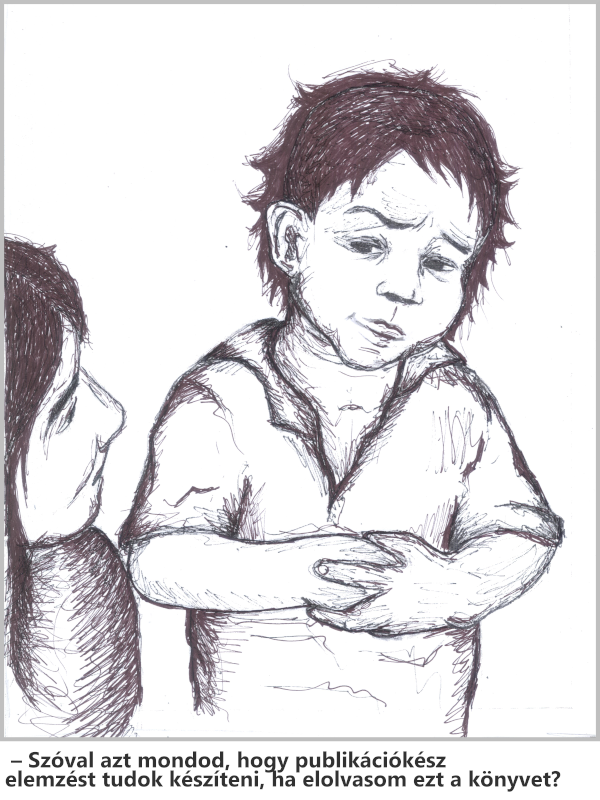
\includegraphics[width=0.7\linewidth]{images/ch_01_small} \end{center}



\hypertarget{Itt-kezdodik-1-szint}{%
\section{Elindulás}\label{Itt-kezdodik-1-szint}}

\begin{rmdlevel1}
Ebben a fejezetben:

\begin{itemize}
\tightlist
\item
  bemutatunk egy konkrét adatelemzési példát,
\item
  áttekintjük a könyv tartalmát,
\item
  lehetőséget adunk az előzetes R ismeretek felmérésére,
\item
  és segítünk a megfelelő fejezet kiválasztására a folytatáshoz.
\end{itemize}
\end{rmdlevel1}

Könyvünk elsődleges célja az R bemutatása kezdő felhasználók számára, de minden bizonnyal azok is találni fognak hasznos részeket, akik már rendelkeznek R ismeretekkel. Bevezetést nyújtunk az R által lefedett három nagy terület mindegyikébe: az adatkezelésbe, a grafikus megjelenítésbe és az adatelemzésbe is. A leírtak megértéséhez a statisztikai alapismereteken túl semmilyen előzetes tudás nem szükséges.

Most egy konkrét adatelemzési példa segítségével bemutatjuk, hogy mit nyújt e könyv az Olvasó számára. A bevezető példa megoldása során az előismeretekkel rendelkező Olvasó a saját R tudását is felmérheti, és ezzel egyben segítséget kaphat a tudásához és céljaihoz legjobban illeszkedő fejezet kiválasztására, amellyel tovább folytathatja az olvasást.

\textbf{Bevezető példa: Két tanítási módszer összehasonlítása}\\
Egy 2020-as kutatásunkban \citep{Csapo2020} 7. osztályos tanulóknak Excel ismereteket oktattunk két különböző megközelítésben. Az egyik csoportban hagyományos, míg a másikban modern (Sprego) tanítási módszert használtunk. A tanulási időszak az Excel ismeretek felmérésével zárult. Az összegyűjtött adatok az \texttt{excel\_2020.xlsx} állományban állnak rendelkezésre.\\
Nézzük az adatelemzés lépéseit és egyben könyvünk felépítését!

\textbf{2. fejezet: Mi az R?}\\
A bevezető példa megoldását R-ben fogjuk elvégezni (és nem más eszközben, mint például az SPSS, jamovi, JASP, SAS stb.). Érdemes tehát ismerni az R céljait és lehetőségeit, jó ha van egy összképünk a használt statisztikai programcsomagról. Ezt az áttekintést nyújtja 2 fejezet.

\textbf{3. fejezet: Az R telepítése.}\\
Az adatelemzés konkrét lépéseinek elvégzéséhez telepített \emph{Alap R} és \emph{RStudio} szükséges. Ha ezek nem állnak rendelkezésre, vagy még nem is találkoztunk ezekkel az eszközökkel, akkor a 3. fejezet nekünk szól.

\textbf{4. fejezet: Munka az R-ben.}\\
Az adatelemzés végrehajtásához az \emph{RStudio}-t ajánljuk, és azon belül pedig a projektek használatát szorgalmazzuk. A 4. fejezetben megismerjük az \emph{RStudio} legalapvetőbb funkcióit, a parancsállományok létrehozását és futtatását.

A fenti előzmények után elkezdhetjük a bevezető példa megoldását:

\begin{enumerate}
\def\labelenumi{\arabic{enumi}.}
\tightlist
\item
  indítsuk el az \emph{RStudio}-t,
\item
  hozzunk létre egy új projektet,
\item
  hozzunk létre egy új RMarkdown állományt,
\item
  helyezzük el a lentebb szereplő R parancsokat az RMarkdown állomány egyes csonkjaiban.
\end{enumerate}

\textbf{5. fejezet: Az R nyelv.}\\
Az R parancsok létrehozásának vannak szabályai, amelyeket a munka során be kell tartanunk. Ismernünk kell jó néhány függvényt, és általában el kell tudnunk igazodni az R nyelvben. Az 5. fejezet ezért kulcsfontosságú, tanulmányozzuk alaposan, és lehetőleg minden kitűzött feladatát oldjuk meg.

\textbf{6. fejezet: Beolvasás}\\
Az adatelemzés első lépése az adatállomány beolvasása. Adataink változatos formában állhatnak rendelkezésre, a 6. fejezetben ezek beolvasására kapunk receptet.

A bevezető példa megoldásához az RMarkdown állomány egyik csonkját bővítsük a lenti sorokkal.

\begin{Shaded}
\begin{Highlighting}[]
\CommentTok{\# install.packages("rio")                         \# rio csomag telepítése}
\FunctionTok{library}\NormalTok{(rio)                                      }\CommentTok{\# rio csomag betöltése}
\NormalTok{felmeres }\OtherTok{\textless{}{-}} \FunctionTok{import}\NormalTok{(}\AttributeTok{file =} \StringTok{"adat/excel\_2020.xlsx"}\NormalTok{) }\CommentTok{\# beolvasás}
\end{Highlighting}
\end{Shaded}

\textbf{7. fejezet: Adatkezelés}\\
A statisztikai elemzés elkezdése előtt számos adatkezelési tevékenységre lehet szükség. Ezt a sokszor rendkívül időigényes folyamatot a 7. fejezetben részletezzük.

A bevezető példa megoldásához az RMarkdown állomány egyik csonkját bővítsük a lenti sorokkal. Az adatkezelés legtöbbször a beolvasott állomány \emph{jellemzőinek lekérésével} kezdődik.

\begin{Shaded}
\begin{Highlighting}[]
\FunctionTok{str}\NormalTok{(felmeres)              }\CommentTok{\# dataframe szerkezete}
\FunctionTok{names}\NormalTok{(felmeres)            }\CommentTok{\# változónevek  }
\FunctionTok{unique}\NormalTok{(felmeres}\SpecialCharTok{$}\NormalTok{modszer)   }\CommentTok{\# különböző értékek {-} osztaly}
\end{Highlighting}
\end{Shaded}

A karakteres vagy numerikus vektorok faktorrá konvertálása az egyik leggyakoribb előkészítő parancs.

\begin{Shaded}
\begin{Highlighting}[]
\NormalTok{felmeres}\SpecialCharTok{$}\NormalTok{modszer }\OtherTok{\textless{}{-}} \FunctionTok{factor}\NormalTok{(felmeres}\SpecialCharTok{$}\NormalTok{modszer)}
\end{Highlighting}
\end{Shaded}

A táblázatok és ábrák megfelelő megjelenéséhez, végezzük el a \emph{faktorszintek sorrendbe állítását}.

\begin{Shaded}
\begin{Highlighting}[]
\NormalTok{felmeres}\SpecialCharTok{$}\NormalTok{modszer }\OtherTok{\textless{}{-}} \FunctionTok{factor}\NormalTok{(felmeres}\SpecialCharTok{$}\NormalTok{modszer, }\AttributeTok{levels=}\FunctionTok{c}\NormalTok{(}\StringTok{"modern"}\NormalTok{, }\StringTok{"hagyományos"}\NormalTok{))}
\end{Highlighting}
\end{Shaded}

\textbf{8. fejezet: Mutatók és táblázatok.}\\
Ha az adatainkat már megfelelő formába hoztuk, akkor továbbléphetünk az elemzés felé. A 8. fejezet a leíró statisztikai elemzésekből a mutatók és a táblázatok létrehozását mutatja be.

Most a felmérés eredményeinek statisztikai mutatóit íratjuk ki a két tanítási módszert használó csoportban.

\begin{Shaded}
\begin{Highlighting}[]
\CommentTok{\# install.packages("psych") \# psych csomag telepítése}
\NormalTok{psych}\SpecialCharTok{::}\FunctionTok{describeBy}\NormalTok{(}\AttributeTok{x =}\NormalTok{ felmeres}\SpecialCharTok{$}\NormalTok{eredmeny, }\AttributeTok{group =}\NormalTok{ felmeres}\SpecialCharTok{$}\NormalTok{modszer, }\AttributeTok{mat=}\NormalTok{T)}
\CommentTok{\#\textgreater{}     item      group1 vars  n      mean        sd    median   trimmed       mad}
\CommentTok{\#\textgreater{} X11    1      modern    1 13 0.6541958 0.1968892 0.6621212 0.6568871 0.2044191}
\CommentTok{\#\textgreater{} X12    2 hagyományos    1 13 0.3800117 0.1272075 0.3628788 0.3913912 0.1190573}
\CommentTok{\#\textgreater{}            min       max     range       skew  kurtosis         se}
\CommentTok{\#\textgreater{} X11 0.32575758 0.9530303 0.6272727 {-}0.2885768 {-}1.189491 0.05460724}
\CommentTok{\#\textgreater{} X12 0.08333333 0.5515152 0.4681818 {-}0.6434813 {-}0.114030 0.03528102}
\end{Highlighting}
\end{Shaded}

\textbf{9. fejezet: Grafika.}\\
A grafikus megjelenítés is a leíró statisztikai elemzés része. A 9. fejezetben részletesebben olvashatunk a publikációkész ábrák létrehozásáról.

Most a numerikus változók esetén használt egyik elterjedt ábrázolási formát, a dobozdiagramot használjuk két tanítási csoport eredményének grafikus összehasonlítására.

\begin{Shaded}
\begin{Highlighting}[]
\FunctionTok{library}\NormalTok{(ggplot2)}
\FunctionTok{ggplot}\NormalTok{(}\AttributeTok{data =}\NormalTok{ felmeres, }\AttributeTok{mapping =} \FunctionTok{aes}\NormalTok{(}\AttributeTok{x=}\NormalTok{modszer, }\AttributeTok{y=}\NormalTok{eredmeny)) }\SpecialCharTok{+} \FunctionTok{geom\_boxplot}\NormalTok{()}
\end{Highlighting}
\end{Shaded}

\begin{center}\includegraphics[width=0.9\linewidth]{01-Itt-kezdodik_files/figure-latex/unnamed-chunk-8-1} \end{center}

\textbf{10. fejezet: Hipotézisvizsgálatok.}\\
A statisztikai hipotézisvizsgálat minden adatelemzés központi része, a gyűjtött adatokból a populációra nézve következtetést vonhatunk le. A 10. fejezetben a leggyakoribb egyváltozós elemzéseket mutatjuk be.

Most Mann-Whitney-próbát hajtunk végre a két tanítási módszer eredményességének összehasonlítására.

\begin{Shaded}
\begin{Highlighting}[]
\FunctionTok{wilcox.test}\NormalTok{(eredmeny}\SpecialCharTok{\textasciitilde{}}\NormalTok{modszer, }\AttributeTok{data=}\NormalTok{felmeres)}
\CommentTok{\#\textgreater{} }
\CommentTok{\#\textgreater{}  Wilcoxon rank sum exact test}
\CommentTok{\#\textgreater{} }
\CommentTok{\#\textgreater{} data:  eredmeny by modszer}
\CommentTok{\#\textgreater{} W = 145, p{-}value = 0.001248}
\CommentTok{\#\textgreater{} alternative hypothesis: true location shift is not equal to 0}
\end{Highlighting}
\end{Shaded}

\textbf{11. fejezet: Publikálás.}\\
Az elemzés eredményének publikációkész formába alakítása az adatelemzési folyamat utolsó lépése. A 11. fejezetben megismerjük azokat a legegyszerűbb folyamatokat, amelyekkel többnyire formanyelvtől függetlenül, publikációkész eredményközlést végezhetünk.

A bevezető példa elemzése során kapott eredmények publikálását segíti, ha a következő sorokkal kiegészítjük a fenti, leíró statisztikai elemzéseket. Egy soronként vett kétdimenziós gyakorisági táblázat és egy háttértárra mentett ábra a lenti sorok eredménye. Végül fordítsuk le az RMarkdown állományt a \textbf{Knit} nyomógomb segítségével. A kapott HTML (vagy Word/PDF) állomány és a háttértáron keletkezett képállomány jelentősen segíti az eredmények publikálását.

\begin{Shaded}
\begin{Highlighting}[]
\NormalTok{knitr}\SpecialCharTok{::}\FunctionTok{kable}\NormalTok{(}\FunctionTok{t}\NormalTok{(psych}\SpecialCharTok{::}\FunctionTok{describeBy}\NormalTok{(}\AttributeTok{x =}\NormalTok{ felmeres}\SpecialCharTok{$}\NormalTok{eredmeny, }\AttributeTok{group =}\NormalTok{ felmeres}\SpecialCharTok{$}\NormalTok{modszer,}
    \AttributeTok{mat =}\NormalTok{ T)), }\AttributeTok{digits =} \DecValTok{3}\NormalTok{, }\AttributeTok{align =} \FunctionTok{c}\NormalTok{(}\StringTok{"c"}\NormalTok{, }\StringTok{"c"}\NormalTok{), }\AttributeTok{format.args =} \FunctionTok{list}\NormalTok{(}\AttributeTok{decimal.mark =} \StringTok{","}\NormalTok{))}
\end{Highlighting}
\end{Shaded}

\begin{tabular}{l|c|c}
\hline
  & X11 & X12\\
\hline
item & 1 & 2\\
\hline
group1 & modern & hagyományos\\
\hline
vars & 1 & 1\\
\hline
n & 13 & 13\\
\hline
mean & 0.6541958 & 0.3800117\\
\hline
sd & 0.1968892 & 0.1272075\\
\hline
median & 0.6621212 & 0.3628788\\
\hline
trimmed & 0.6568871 & 0.3913912\\
\hline
mad & 0.2044191 & 0.1190573\\
\hline
min & 0.32575758 & 0.08333333\\
\hline
max & 0.9530303 & 0.5515152\\
\hline
range & 0.6272727 & 0.4681818\\
\hline
skew & -0.2885768 & -0.6434813\\
\hline
kurtosis & -1.189491 & -0.114030\\
\hline
se & 0.05460724 & 0.03528102\\
\hline
\end{tabular}

A bevezető példa megoldásához természetesen a hipotézisvizsgálat szöveges értékelés is hozzátartozik, de ezt most az alfejezet végén szereplő egyik kitűzött feladatra halasztjuk. A hangsúly a könyv vázlatos tartalomjegyzékének bemutatásán volt, részletesebb, de felsorolásszerű tartalomjegyzéket a következő két alfejezetben találunk.

\hypertarget{itt-kezdodik-1-summary}{%
\subsection{Összefoglalás}\label{itt-kezdodik-1-summary}}

\begin{rmdsummary}
Ebben az alfejezetben egy adatelemzési példát oldottunk meg, melynek
segítségével illusztrálni tudtuk a további alfejezetek tartalmát. A 2.
fejezetben áttekintést fogunk adni az R-ről, a 3.-ban az \emph{Alap R}
és \emph{RStudio} telepítését, a 4.-ben az \emph{RStudio} használatát
mutatjuk be. Az 5. fejezetben kellő részletességgel ismertetjük az R
nyelvet. A további fejezetekben az adatelemzés szokásos lépéseit vesszük
sorra, a 6. fejezetben a beolvasást, a 7. fejezetben az adatok
előkészítését, a 8. és 9. fejezetben a leíró statisztikai műveleteket
mutatjuk be. A 10. fejezet az egy- és kétváltozós hipotézisvizsgálatoké,
az utolsó 11. fejezet az eredmények publikálását foglalja össze.
\end{rmdsummary}

\hypertarget{itt-kezdodik-1-exercise}{%
\subsection{Feladatok}\label{itt-kezdodik-1-exercise}}

\begin{rmdexercise}
\begin{enumerate}
\def\labelenumi{\arabic{enumi}.}
\tightlist
\item
  Milyen online vagy nyomtat könyvek segítik az R elsajátítását?
  Próbáljuk összegyűjteni a magyar nyelvű könyveket is!
\item
  Térképezzük fel az online videókurzusokat is az R tanulásához!
\item
  A bevezető példa (\emph{Két tanítási módszer összehasonlítása})
  megoldásában a hipotézisvizsgálat alapján adjunk szöveges értékelést!
\end{enumerate}
\end{rmdexercise}

\hypertarget{a-kuxf6nyv-feluxe9puxedtuxe9se}{%
\section{A könyv felépítése}\label{a-kuxf6nyv-feluxe9puxedtuxe9se}}

\begin{rmdlevel2}
Ebben a fejezetben:

\begin{itemize}
\tightlist
\item
  bemutatjuk a könyv részletes felépítését,
\item
  ezzel tovább segítjük a választást a folytatáshoz.
\end{itemize}
\end{rmdlevel2}

A könyv 11 fejezetből áll, és fejezetenként 3 vagy több alfejezetből. Most röviden bemutatjuk az egyes alfejezetek tartalmát.

\begingroup\fontsize{10}{11}\selectfont

\begin{longtable}[]{@{}
  >{\raggedright\arraybackslash}p{(\columnwidth - 2\tabcolsep) * \real{0.34}}
  >{\raggedright\arraybackslash}p{(\columnwidth - 2\tabcolsep) * \real{0.66}}@{}}
\toprule
\begin{minipage}[b]{\linewidth}\raggedright
Fejezet/alfejezet
\end{minipage} & \begin{minipage}[b]{\linewidth}\raggedright
Leírás
\end{minipage} \\
\midrule
\endhead
\textbf{1. Itt kezdődik} & \\
1.1. Elindulás & A könyv fejezeteinek bemutatása egy konkrét adatelemzésen keresztül \\
1.2. A könyv felépítése & A könyv egyes alfejezeteinek rövid bemutatása (jelen alfejezet) \\
1.3. Próbák listája & A könyvben szereplő egy- és kétváltozós statisztikai eljárások listája \\
& \\
\textbf{2. Mi az R?} & \\
2.1. Az R bemutatása & A parancssoros R jellemzői, az R nyelv, az \emph{Alap R} és a csomag fogalma \\
2.2. A modern R & Megtanuljuk a \emph{Tidyverse R} fogalmát, megtudjuk mi a modern R \\
2.3. Múlt és jelen & Az R rövid története, alapelvek az R tanulásához, és az R alaptudás elemei \\
& \\
\textbf{3. Az R telepítése} & \\
3.1. Az Alap R és az RStudio telepítése & Megismerjük az \emph{Alap R} és az \emph{RStudio} telepítését \\
3.2. A Tidyverse R telepítése & A \textbf{tidyverse} csomag(gyűjtemény) telepítése \\
3.3. Az R frissítése & Az \emph{Alap R}, az \emph{RStudio} és a csomagok frissítésének módszerei \\
& \\
\textbf{4. Munka az R-ben} & \\
4.1. Az RStudio használata & Az \emph{RStudio} jellemzői és felépítése, a projektek használata és a segítségkérés \\
4.2. Segítség az R használatához & Segítségkérési lehetőségek az R-ben, a beépített súgó használata \\
4.3. Az Alap R használata & Az \emph{Alap R} konzola, az \emph{RGui}, az \emph{R Commander} és a kötegelt üzemmód lehetőségei \\
& \\
\textbf{5. Az R nyelv} & \\
& \\
\textbf{6. Beolvasás} & \\
& \\
\textbf{7. Adatmanipuláció} & \\
& \\
\textbf{8. Mutatók és táblázatok} & \\
& \\
\textbf{9. Grafika} & \\
& \\
\textbf{10. Hipotézisvizsgálatok} & \\
& \\
\textbf{11. Publikáció} & \\
\bottomrule
\end{longtable}

\endgroup{}

\begin{rmdsummary}
\textbf{Összefoglalás}

Ebben a részben röviden bemutattuk a könyv összes alfejezetét. A
későbbiekben térképként használhatja az Olvasó az itt ismertetett
táblázatot.
\end{rmdsummary}

\begin{rmdexercise}
\textbf{Feladatok}

\begin{enumerate}
\def\labelenumi{\arabic{enumi}.}
\tightlist
\item
  Az adatfeldolgozás 4 lépése a következő: (1) adatok beolvasása, (2) adatok előkészítése elemzésre, (3) adatok elemzése és (4) az eredmények publikálása. A könyv mely fejezetei tartoznak az adatfeldolgozás fenti lépéseihez?
\item
  Az R-rel való munka általunk javasolt módja: \emph{RStudio}-ban, projektmódban, R vagy RMarkdown állományokat szerkesztünk és hajtunk végre. Mely fejezetekben találunk hasznos információkat az R ezen használatával kapcsolatban?
\end{enumerate}
\end{rmdexercise}

\hypertarget{pruxf3buxe1k-listuxe1ja}{%
\section{Próbák listája}\label{pruxf3buxe1k-listuxe1ja}}

\begin{rmdlevel3}
Ebben a fejezetben:

\begin{itemize}
\tightlist
\item
  áttekintést adunk az egy- és kétváltozós hipotézisvizsgálatokról.
\end{itemize}
\end{rmdlevel3}

A 10. fejezetben bemutatjuk az egy- és kétváltozós hipotézisvizsgálatok végrehajtását. Ebben a fejezetben felsoroljuk a legfontosabb próbákat, összesen öt táblázatban soroljuk fel őket:

\begin{itemize}
\tightlist
\item
  egy mintát vizsgáló próbák (\ref{tab:egyminta1} táblázat),
\item
  páros mintát vizsgáló próbák (\ref{tab:parosminta1} táblázat),
\item
  két független mintát vizsgáló próbák (\ref{tab:ketminta1} táblázat),
\item
  több összetartozó mintát vizsgáló próbák (\ref{tab:tobbosszeminta1} táblázat),
\item
  több független mintát vizsgáló próbák (\ref{tab:tobbminta1} táblázat).
\end{itemize}

A táblázatokban megadjuk, hogy a vizsgálatnak mi a célja, vagyis a populációbeli változó(k) melyik paraméterére vonatkoznak a próbák, a várható értékre, a mediánra, a varianciára vagy a valószínűségre. A 10. fejezetben foglalkozunk az eloszlásvizsgálatok közül a normalitást ellenőrző próbákkal is, így a \ref{tab:egyminta1} táblázat ezeket is számba veszi.

\begin{longtable}[]{@{}
  >{\raggedright\arraybackslash}p{(\columnwidth - 4\tabcolsep) * \real{0.21}}
  >{\raggedright\arraybackslash}p{(\columnwidth - 4\tabcolsep) * \real{0.48}}
  >{\raggedright\arraybackslash}p{(\columnwidth - 4\tabcolsep) * \real{0.31}}@{}}
\caption{\label{tab:egyminta1} Egy minta vizsgálata}\tabularnewline
\toprule
\begin{minipage}[b]{\linewidth}\raggedright
Cél
\end{minipage} & \begin{minipage}[b]{\linewidth}\raggedright
Próba neve
\end{minipage} & \begin{minipage}[b]{\linewidth}\raggedright
R függvény
\end{minipage} \\
\midrule
\endfirsthead
\toprule
\begin{minipage}[b]{\linewidth}\raggedright
Cél
\end{minipage} & \begin{minipage}[b]{\linewidth}\raggedright
Próba neve
\end{minipage} & \begin{minipage}[b]{\linewidth}\raggedright
R függvény
\end{minipage} \\
\midrule
\endhead
várható érték & egymintás u-próba & \texttt{BSDA::z.test()} \\
& egymintás t-próba & \texttt{t.test()} \\
medián & előjel-próba & \texttt{BSDA::SIGN.test()} \\
& Mood-féle medián-próba & \\
& egymintás Wilcoxon-próba & \texttt{wilcox.test()} \\
variancia & khí-négyzet próba & \texttt{chisq.test()} \\
valószínűség & khí-négyzet próba & \texttt{chisq.test()} \\
normalitás & Shapiro-Wilk próba & \texttt{shapiro.test()} \\
& Kolmogorov-Szmirnov próba & \texttt{DescTools:LillieTest()} \\
\bottomrule
\end{longtable}

\begin{longtable}[]{@{}
  >{\raggedright\arraybackslash}p{(\columnwidth - 4\tabcolsep) * \real{0.21}}
  >{\raggedright\arraybackslash}p{(\columnwidth - 4\tabcolsep) * \real{0.48}}
  >{\raggedright\arraybackslash}p{(\columnwidth - 4\tabcolsep) * \real{0.31}}@{}}
\caption{\label{tab:parosminta1} Páros minta vizsgálata}\tabularnewline
\toprule
\begin{minipage}[b]{\linewidth}\raggedright
Cél
\end{minipage} & \begin{minipage}[b]{\linewidth}\raggedright
Próba neve
\end{minipage} & \begin{minipage}[b]{\linewidth}\raggedright
R függvény
\end{minipage} \\
\midrule
\endfirsthead
\toprule
\begin{minipage}[b]{\linewidth}\raggedright
Cél
\end{minipage} & \begin{minipage}[b]{\linewidth}\raggedright
Próba neve
\end{minipage} & \begin{minipage}[b]{\linewidth}\raggedright
R függvény
\end{minipage} \\
\midrule
\endhead
várható érték & páros t-próba & \texttt{t.test(paired=T)} \\
medián & páros előjel-próba & \texttt{BSDA::SIGN.test()} \\
& páros Wilcoxon-próba & \texttt{wilcox.test(paired=T)} \\
variancia & & \texttt{var.test()} \\
valószínűség & McNemar-próba & \texttt{mcnemar.test()} \\
& Cohran-Q próba & \texttt{mcnemar.test()} \\
\bottomrule
\end{longtable}

\begin{longtable}[]{@{}
  >{\raggedright\arraybackslash}p{(\columnwidth - 4\tabcolsep) * \real{0.21}}
  >{\raggedright\arraybackslash}p{(\columnwidth - 4\tabcolsep) * \real{0.48}}
  >{\raggedright\arraybackslash}p{(\columnwidth - 4\tabcolsep) * \real{0.31}}@{}}
\caption{\label{tab:ketminta1} Két független minta vizsgálata}\tabularnewline
\toprule
\begin{minipage}[b]{\linewidth}\raggedright
Cél
\end{minipage} & \begin{minipage}[b]{\linewidth}\raggedright
Próba neve
\end{minipage} & \begin{minipage}[b]{\linewidth}\raggedright
R függvény
\end{minipage} \\
\midrule
\endfirsthead
\toprule
\begin{minipage}[b]{\linewidth}\raggedright
Cél
\end{minipage} & \begin{minipage}[b]{\linewidth}\raggedright
Próba neve
\end{minipage} & \begin{minipage}[b]{\linewidth}\raggedright
R függvény
\end{minipage} \\
\midrule
\endhead
várható érték & kétmintás u-próba & \texttt{BSDA::z.test()} \\
& kétmintás t-próba & \texttt{t.test()} \\
& Welch-féle d-próba & \texttt{t.test(var.equal=F)} \\
medián & Mann--Whitney-próba & \texttt{wilcox.test()} \\
variancia & F-próba & \texttt{var.test()} \\
valószínűség & khí-négyzet próba & \texttt{chisq.test()} \\
& Fisher-féle egzakt próba & \texttt{fisher.test()} \\
\bottomrule
\end{longtable}

\begin{longtable}[]{@{}
  >{\raggedright\arraybackslash}p{(\columnwidth - 4\tabcolsep) * \real{0.26}}
  >{\raggedright\arraybackslash}p{(\columnwidth - 4\tabcolsep) * \real{0.42}}
  >{\raggedright\arraybackslash}p{(\columnwidth - 4\tabcolsep) * \real{0.29}}@{}}
\caption{\label{tab:tobbosszeminta1} Több összetartozó minta vizsgálata}\tabularnewline
\toprule
\begin{minipage}[b]{\linewidth}\raggedright
Cél
\end{minipage} & \begin{minipage}[b]{\linewidth}\raggedright
Próba neve
\end{minipage} & \begin{minipage}[b]{\linewidth}\raggedright
R függvény
\end{minipage} \\
\midrule
\endfirsthead
\toprule
\begin{minipage}[b]{\linewidth}\raggedright
Cél
\end{minipage} & \begin{minipage}[b]{\linewidth}\raggedright
Próba neve
\end{minipage} & \begin{minipage}[b]{\linewidth}\raggedright
R függvény
\end{minipage} \\
\midrule
\endhead
várható érték & \begin{minipage}[t]{\linewidth}\raggedright
egyszempontos összetartozó\\
mintás varianciaelemzés\strut
\end{minipage} & \texttt{ez::ezANOVA()} \\
medián & Friedman-próba & \texttt{friedman.test()} \\
\bottomrule
\end{longtable}

\begin{longtable}[]{@{}
  >{\raggedright\arraybackslash}p{(\columnwidth - 4\tabcolsep) * \real{0.21}}
  >{\raggedright\arraybackslash}p{(\columnwidth - 4\tabcolsep) * \real{0.48}}
  >{\raggedright\arraybackslash}p{(\columnwidth - 4\tabcolsep) * \real{0.31}}@{}}
\caption{\label{tab:tobbminta1} Több független minta vizsgálata}\tabularnewline
\toprule
\begin{minipage}[b]{\linewidth}\raggedright
Cél
\end{minipage} & \begin{minipage}[b]{\linewidth}\raggedright
Próba neve
\end{minipage} & \begin{minipage}[b]{\linewidth}\raggedright
R függvény
\end{minipage} \\
\midrule
\endfirsthead
\toprule
\begin{minipage}[b]{\linewidth}\raggedright
Cél
\end{minipage} & \begin{minipage}[b]{\linewidth}\raggedright
Próba neve
\end{minipage} & \begin{minipage}[b]{\linewidth}\raggedright
R függvény
\end{minipage} \\
\midrule
\endhead
várható érték & egyszempontos varianciaelemzés & \texttt{aov()} \\
& Welch-féle egyszempontos varianciaelemzés & \texttt{oneway.test(var.equal=F)} \\
medián & Kruskal--Wallis-próba & \texttt{kruskal.test()} \\
variancia & Levene-próba & \texttt{DescTools::LeveneTest()} \\
& Bartlett-próba & \texttt{bartlett.test()} \\
\bottomrule
\end{longtable}

\begin{rmdsummary}
\textbf{Összefoglalás}

Ebben a részben rövid áttekintést adtunk a könyv 10. fejezetében sorra
kerülő statisztikai próbákról. Megneveztük a próbákat, R parancsokkal
szemléltettük használatukat, valamint jeleztük a céljukat. A táblázatok
áttekintésével képet kaphatunk arról, hogy a későbbiekben milyen jellegű
statisztikai következtetéseket tudunk levonni az R használatával.
\end{rmdsummary}

\begin{rmdexercise}
\textbf{Feladatok}

\begin{enumerate}
\def\labelenumi{\arabic{enumi}.}
\tightlist
\item
  Minden statisztikai próba esetében négy dolgot érdemes tudni: (1) a statisztikai próba neve, (2) null- és ellenhipotézise, (3) alkalmazási feltételei, és (4) a próba végrehajtásának módja valamely statisztikai programcsomagban. A 10. fejezetben a statisztikai próbák végrehajtását természetesen R-beli eszközökkel mutatjuk be. Ismerjük a fenti táblázatokban megnevezett próbák null- és ellenhipotézisét, valamint az alkalmazási feltételeit? Próbáljuk ezeket felidézni! Hol találunk ezekről információt?
\item
  Mely próbák maradtak ki ebből a könyvből? Hol találunk ezek R-beli végrehajtására példát?
\end{enumerate}
\end{rmdexercise}

\hypertarget{mi-az-r}{%
\chapter{Mi az R?}\label{mi-az-r}}

\begin{center}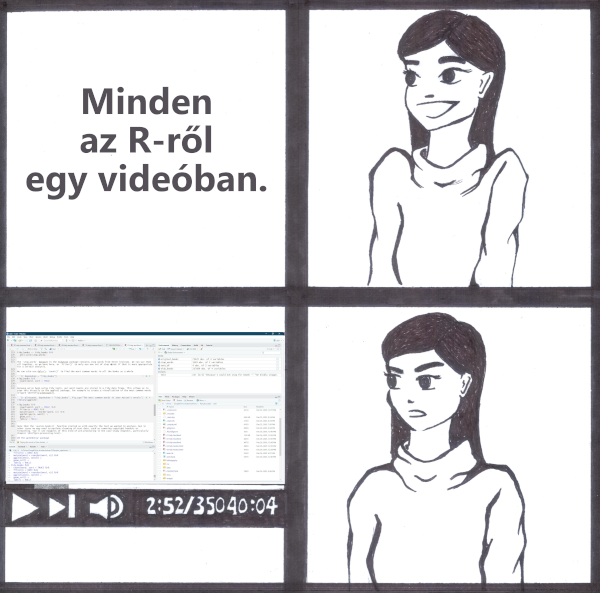
\includegraphics[width=0.6\linewidth]{images/ch_02_small} \end{center}

\hypertarget{az-r-bemutatuxe1sa}{%
\section{Az R bemutatása}\label{az-r-bemutatuxe1sa}}

\begin{rmdlevel1}
Ebben a fejezetben:

\begin{itemize}
\tightlist
\item
  megismerjük az R jellemzőit,
\item
  megtudjuk, hogy melyek a parancssoros interfész előnyei,
\item
  megismerjük az \emph{Alap R} fogalmát,
\item
  körülhatároljuk az R nyelv, az \emph{Alap R} és a csomag fogalmát.
\end{itemize}
\end{rmdlevel1}

\hypertarget{az-r-jellemzux151i}{%
\subsection{Az R jellemzői}\label{az-r-jellemzux151i}}

Az R egy magas szintű programozási nyelv és környezet, amelynek legfontosabb felhasználása az adatelemzés és az ahhoz kapcsolódó grafikus megjelenítés. Három alapvető jellemzője kiemeli a többi statisztikai programcsomag közül: (1) az R ingyenesen telepíthető és használható; (2) az R nyílt forrású, így bárki hozzájárulhat az R fejlesztéséhez, azaz létrehozhat új \emph{csomag}okat, és ezzel kiegészítheti az R tudását; és (3) az R felhasználók rendkívül aktív és befogadó online közösséget alkotnak, szinte minden felmerülő kérdésünkre hamar választ kaphatunk.

Álljon itt egy bővített lista azokról a jellemzőkről, amelyek vonzóvá tehetik számunkra az R statisztikai programcsomagot.

\begin{itemize}
\tightlist
\item
  Az R szabad szoftver, bárki ingyenesen letöltheti és használhatja. Ez egyfelől megkönnyíti az oktatási intézmények, tanszékek és oktatók munkáját, hiszen nincs szükség a kereskedelmi programok licenszeléséből adódó pénzügyi vagy más természetű nehézségek kezelésére. Másrészt a hallgatók a statisztika kurzusok során tanultakat otthon vagy később a munkájukban is felhasználhatják.
\item
  Az R platform-független, azaz Windows, Linux és macOS környezetben is használható. Nem kell lemondanunk a kedvenc operációs rendszerünkről, ha az R-t szeretnénk használni.
\item
  Az R egy teljes értékű programozási nyelv, nem csak egy statisztikai programcsomag önmagában.
\item
  Az R statisztikai módszerek szinte végtelen választékát kínálja. A R-ben felhasználható statisztikai eljárásokat statisztikusok fejlesztik folyamatosan és csomagok formájában teszik elérhetővé. Valószínű, hogy egy új statisztikai módszer leghamarabb az R-ben válik elérhetővé.
\item
  Az R rendkívül gazdag grafikus lehetőségekkel rendelkezik.
\item
  A statisztikai szakirodalomban és az egyetemi oktatók körében egyre elterjedtebb az R, mint közös (statisztikai program)nyelv használata. Ha valamilyen statisztikai problémára keressük a megoldást, vagy csak konzultálunk egy statisztikussal, az R ismerete (akár csak olvasási szinten) rendkívüli előnyt jelenthet.
\item
  Az R igen jól dokumentált, a beépített súgón kívül számos könyv és leírás érhető el.
\item
  Az R parancssoros interfésszel rendelkezik, amely számos előnnyel jár. Egyrészt a szkript állományok létrehozása és végrehajtása a statisztikai elemzések megismételhetőségét biztosítják, másrészt ez az oktatók és a hallgatók könnyebb kommunikációját is lehetővé teszi.
\item
  Az R az adatelemzés eredményének sokszínű publikálását is biztosítja. Az \href{https://rmarkdown.rstudio.com/}{RMarkdown} formanyelv segítségével HTML, PDF és Word dokumentumot, illetve prezentációs diákat vagy akár kész cikkeket hozhatunk létre. A \href{http://shiny.rstudio.com/}{Shiny} csomag interaktív Webes alkalmazások építését teszi lehetővé.
\item
  Mára az R használata szinte egyet jelent az ingyenesen elérhető \href{https://www.rstudio.com/}{\emph{RStudio}} használatával, amely egy kényelmes integrált fejlesztői környezetet biztosít a parancsállományok létrehozásához.
\end{itemize}

Érdemes bepillantani az R árnyékosabb oldalába is. Az R egyik gyengesége, hogy nagy adatbázisok kezeléséhez erős hardverre van szüksége, de a legtöbb felhasználás során ez semmilyen problémát nem okoz. A másik gyengeség, hogy az R elsajátításához nem kevés idő és kitartás szükséges. Jelen könyv éppen ezt a folyamatot kívánja megkönnyíteni és lerövidíteni.

\hypertarget{a-r-parancssoros}{%
\subsection{A R parancssoros}\label{a-r-parancssoros}}

Az R alapvető használata során parancsokat gépelünk be és hajtunk végre. Ez lényegesen eltér a ma megszokott felhasználói programok világától, ahol egy grafikus felhasználói felületen egérrel vagy az ujjunkkal mutogatjuk el a kívánt tevékenységet. Az R egészen más megközelítést vall, használata a kezdeti lépésektől nagyfokú figyelmet és pontosságot követel. A parancsokban kell gondolkodnunk, ám ezt végig áthatja a \emph{tudom mit csinálok} elv, így némi idő elteltével érezni fogjuk, hogy az R megszelídül, már nem köt bele minden ``szavunkba'', egyre több dologra tudjuk rávenni, és végül egy rendkívül értékes társsá válik. Jelen könyv ezen az úton szeretné végigvezetni az Olvasót.

Már a tanulás elején szeretnénk tisztázni, hogy az R elsajátításához nem szükséges programozói alaptudás. Az R felhasználók többsége egyáltalán nem programozó, és a mindennapi adatelemző munka sem igényli az R nyelv programozói fokú ismeretét. Természetesen, ha rendelkezünk ilyen irányú előtanulmányokkal a tanulási folyamat néhány szakasza lerövidíthető, de könyvünk elsősorban azok számra íródott, akik programozási nyelvekkel korábban nem találkoztak, és nem is vágynak az R ilyen mélységű ismeretére. Az R nyelv elsajátítása során bevezetjük azokat az egyszerű fogalmakat, amelyeket nem nélkülözhetők az adatelemzés során, azonban az R programozásához más szakkönyveket javaslunk olvasásra.

\hypertarget{mi-valuxf3juxe1ban-az-r}{%
\subsection{Mi valójában az R?}\label{mi-valuxf3juxe1ban-az-r}}

Az R nyelv fejlesztője az \href{https://www.r-project.org/contributors.html}{R Core Team}. Az R nyelv egy rendkívül népszerű szkriptnyelv, több millióan használják világszerte. Elsősorban adatelemzésre, adatmodellezésre és grafikus megjelenítésre, vagyis arra, amit ma adattudományok (data science) alatt értünk. Azonban az R nyelv önmagában nem szoftver, hanem egy rendkívül rugalmas szkriptnyelv, amely például előírja, hogy milyen szintaktikai szabályok mentén fogalmazhatjuk meg az utasításainkat. Ahhoz, hogy az R nyelvet használni tudjuk, vagyis, hogy a számítógép valóban végre is hajtsa a szintaktikailag helyes utasításinkat, szükség van egy szoftveres környezetre, egy olyan futtató rendszerre, amely a kódunkat értelmezi és végrehajtja.

Az R környezet három fő összetevőt tartalmaz: (1) egy \emph{konzol}t, ahová a parancsainkat begépelhetjük; (2) a parancsok végrehajtásáért felelős \emph{R interpreter}t; (3) a \emph{csomagokok}at. A konzol és az interpreter biztosítja az R nyelven írt parancsok tényleges végrehajtását. Így tudunk adatokat beolvasni, átlagot számolni, varianciaelemzést futtatni, vagy publikációkész ábrákat létrehozni. A csomagok adatokat és függvényeket tartalmaznak, például a \textbf{MASS} csomag 88 adatobjektumot és 78 függvényt tartalmaz. A függvények valamilyen tevékenységet hajtanak végre, és valójában ezeket a csomag-függvényeket használjuk fel a konzolban, ha \emph{bármilyen tevékenységet} szeretnénk végrehajtani (például adatokat beolvasni, átlagot számolni stb.). A könyv írásának időpontjában kb. 17000 csomag volt érhető el az R-hez. Csomagok 3 csoportját különböztetjük meg: \emph{standard csomagok} (14 db), \emph{ajánlott csomagok} (15 db) és \emph{egyéb csomagok} (kb. 17000 db). A standard csomagok fejlesztője az R Core Team. A standard csomagok: \textbf{base}, \textbf{compiler}, \textbf{datasets}, \textbf{grDevices}, \textbf{graphics}, \textbf{grid}, \textbf{methods}, \textbf{parallel}, \textbf{splines}, \textbf{stats}, \textbf{stats4}, \textbf{tcltk}, \textbf{tools}, \textbf{utils}. Az ajánlott csomagok: \textbf{KernSmooth}, \textbf{MASS}, \textbf{Matrix}, \textbf{boot}, \textbf{class}, \textbf{cluster}, \textbf{codetools}, \textbf{foreign}, \textbf{lattice}, \textbf{mgcv}, \textbf{nlme}, \textbf{nnet}, \textbf{rpart}, \textbf{spatial}, \textbf{survival}. Az ajánlot csomagok közül a \textbf{foreign} és az \textbf{nlme} fejlesztője az R Core Team, a többit más felhasználók fejlesztették, például a már említett \textbf{MASS} csomag fejlesztője Brian Ripley. Csomagot bárki szabadon fejleszthet és terjeszthet, az \emph{egyéb csomagok} csoportját akár mi is gyarapíthatjuk.

A R környezet már igazi szoftver, terjesztésének koordinálását az \href{https://www.r-project.org/foundation/}{R Foundation} végzi a \href{https://cran.r-project.org/mirrors.html}{CRAN} infrastruktúráján keresztül. Ez biztosítja, hogy számítógépünkre telepíthessük az R környezetet. Ezt a CRAN-ról elérhető R futtatási környezetet \emph{Alap R}-nek nevezzük. Fő komponensei a már említett konzol a parancsok begépelésére, az R értelmező a begépelt parancsok végrehajtására és a csomagok közül a standard és ajánlott csomagok. Az \emph{Alap R} telepítése után már tudunk R parancsokat végrehajtani, és nagyon sok adatelemzési probléma megoldására nyílik módunk, sőt azt mondhatjuk, hogy tetszőleges problémát megoldhatunk kisebb-nagyobb erőfeszítéssel, mert az R egy teljes értékű nyelv. Azonban sokszor érdemesebb az \emph{egyéb csomagok} közül választani, hiszen könnyen elképzelhető, hogy a számtalan csomag között találunk olyat, amely segítségünkre lehet speciális feladataink megoldása során. Valószínű, hogy létezik olyan csomago és benne olyan függvény, amely adatkezelési, adatelemzési, grafikai vagy publikálási feladatunkat jelentősen megkönnyíti. Az \emph{egyéb csomagok} csoportjába tartozó csomagok forrása több tárhely is lehet, ezek közül legjelentősebb az R Foundation által karbantartott CRAN (kb. 15000 csomaggal), a Bioconductor (1741 csomaggal) és a GitHub.

Az R tehát egyszerre több dolgot jelent. Az R egyrészt egy magas szintű programozási nyelv, hamarosan megtanuljuk, hogyan írjunk ezen a nyelven értelmes utasításokat. Másrészt a nyelv körüli környezetet is jelenti, amely magába foglalja a konzolt, a parancsaink értelmezésért felelős R interpretert, valamint azokat a csomagokat, amelyekkel az R tudása kiegészíthető.

\begin{rmdsummary}
\textbf{Összefoglalás}

Minden statisztikai programcsomag, így az R is, alapvetően a
számításigényes statisztikai eljárások kézi végrehajtásától kímél meg
minket. Az R nagyon gazdag adatmanipulációs és grafikus funkciókban is,
támogatja a reprodukálható adatelemzés végrehajtását. Az R ingyenes,
többplatformos és egyik legfontosabb jellemzője, hogy parancsok útján
bírhatjuk működésre. Az \emph{Alap R} biztosítja a konzolt a parancsok
begépelésére, az R interpretert a parancsok tényleges végrehajtására, és
jónéhány csomagba szervezett eljárást az adatelemzési feladatok
elvégzéséhez. Az \emph{Alap R} mindössze néhány tucat csomagot
tartalmaz, \emph{standard csomagokokat} és az \emph{ajánlott
csomagokat}, de több tízezer további csomaggal bővíthetjük az R tudását.
Az adatelemzési munka során egy R környezet vesz minket körül, amely az
R nyelven megírt parancsok értelmezésére és végrehajtására képes
\emph{Alap R}-ből, és az ún. \emph{egyéb csomagokból} áll.
\end{rmdsummary}

\begin{rmdexercise}
\textbf{Feladatok}

\begin{enumerate}
\def\labelenumi{\arabic{enumi}.}
\tightlist
\item
  Keressünk weboldalakat, amelyek az R előnyeit és hátrányait listázzák!
\item
  Keressük meg, hogy az R optimális futtatásához, milyen hardver követelmények szükségesek!
\item
  Nézzünk utána, hogy ma kb. hány csomag érhető el az R-hez? Keressünk ábrát, amely bemutatja, hogy az évek során hány csomag volt elérhető az R-hez?
\item
  Hol áll az R népszerűsége a többi programozási nyelvhez, illetve statisztikai programcsomaghoz képest?
\item
  Milyen ingyenesen elérhető, grafikus felhasználói felülettel rendelkező statisztikai programcsomagok építenek az R-re?
\item
  Említettük, hogy az adatelmezési munka nem igényli az R programozói fokú ismeretét, de soroljunk fel néhány könyvet, amelyből az R programozása is megtanulható!
\end{enumerate}
\end{rmdexercise}

\hypertarget{a-modern-r}{%
\section{A modern R}\label{a-modern-r}}

\begin{rmdlevel2}
Ebben a fejezetben:

\begin{itemize}
\tightlist
\item
  megismerjük a \emph{Tidyverse R} fogalmát,
\item
  megtudjuk mit értünk modern R alatt.
\end{itemize}
\end{rmdlevel2}

A 2014-es év az R nyelv életében meghatározó változást hozott. Egyrészt megjelent a \textbf{magrittr} csomagban a pipe operátor (\texttt{\%\textgreater{}\%}), amellyel olvashatóbb kódok írására nyílt lehetőség\footnote{\url{https://www.r-bloggers.com/magrittr-simplifying-r-code-with-pipes/}}, másrészt a pipe operátorra alapozva Hadley Wickham bemutatta a \textbf{dplyr} és \textbf{tidyr} csomagokat. Ezzel az R funkcionális\footnote{Az R egy nem túl fiatal, a funkcionális programnyelvekhez hasonlóan építkező programozási nyelv, vagyis egy probléma megoldása tipikusan sokszorosan egymásba ágyazott függvényhívások segítségével történik. Ez sok-sok nyitó és záró kerekzárójellel jár együtt, így a parancsaink áttekintése és karbantartása sokszor nehézségekbe ütközik. Ezt kiküszöbölendő az R-ben előszeretettel használnak procedurális eszközöket (például \texttt{for} ciklusokat), de a kód olvashatóságát és karbantartását igazán ez sem könnyíti meg.} oldalát úgy erősítették meg\footnote{\url{https://www.r-bloggers.com/magrittr-the-best-thing-to-have-ever-happened-to-r/}}, hogy a sokszoros egymásba ágyazás során kiküszöbölték a kerekzárójelek írásának problémáját. Az ebben a szellemben készült csomagok listája bővült az idők folyamán, és a \emph{Tidyverse} nevet kapta ez a csomaggyűjtemény. Jelenleg a következő csomagok alkotják: \textbf{ggplot2}, \textbf{purrr}, \textbf{tibble}, \textbf{dplyr}, \textbf{tidyr}, \textbf{stringr}, \textbf{readr} és \textbf{forcats}. Ezek a csomagok nem egyszerűen új funkciókkal ruházzák fel az \emph{Alap R} tudását, mint általában az \emph{egyéb csomagok}. A \emph{Tidyverse} csomagjai konzisztens módon együttműködnek, és egy új megközelítést hoznak az adatelemzési folyamatok végrehajtásában és a kódok írásában. Rövidebb idő alatt hozhatunk létre könnyebben karbantartható kódokat, és a műveleteink végrehajtása is rendszerint gyorsabb. Amikor ebben a megközelítésben hozzuk létre és hajtjuk végre utasításainkat, akkor azt mondjuk hogy a \emph{Tidyverse R}-t használjuk. A \emph{Tidyverse R} nem helyettesíti az \emph{Alap R}-t, és csak bizonyos feladatokra használható. Lássunk tisztán, amit elvégezhetünk \emph{Tidyverse R}-ben, azt az \emph{Alap R}-ben is meg tudnánk tenni, de valószínűleg több gépeléssel, lassabb és rosszabbul karbantartható kóddal.

Eddig láttuk, hogy az R használatához szükséges az \emph{Alap R} telepítése, majd a speciális problémánknak megfelelően kiegészíthetjük az R tudását úgy, hogy telepítünk egyet vagy többet az \emph{egyéb csomagok} kategóriájából. Választhatjuk akár a \emph{Tidyverse} csomagjait is telepítésre, ugyanis így lehetőségünk nyílik a \emph{Tidyverse R} használatára. Utasításaink megfogalmazásának ma ez a legmodernebb módja.

A modern R alatt lényegében azokat a funkciókat értjük, amelyek a \href{https://www.tidyverse.org/}{\emph{Tidyverse}} gyűjteményben található csomagokhoz kötődnek. Ezekkel a csomagokkal, gyorsabb, olvashatóbb és könnyebben karbantartható kódokat hozhatunk létre. A \emph{Tidyverse} használata tehát erősen javasolt, de ebben a könyvben a ``hagyományos'', \emph{Tidyverse R} előtti lehetőségeket is bemutatjuk.

\begin{rmdsummary}
\textbf{Összefoglalás}

A \emph{Tidyverse R} egy csomaggyűjtemény az \emph{egyéb csomagok}
csoportjából, amely újabb szemléletű R parancsok írására ad lehetőséget.
Az így készült kódjaink rendszerint gyorsabban futnak és könnyebben
karbantarthatók. A modern R a \emph{Tidyverse R} csomagjaival
kiegészített \emph{Alap R}, de legfőképp egy új lehetőség parancsaink
megfogalmazására.
\end{rmdsummary}

\begin{rmdexercise}
\textbf{Feladatok}

\begin{enumerate}
\def\labelenumi{\arabic{enumi}.}
\tightlist
\item
  Ki Hadley Wickham?
\item
  Honnan származik a pipe operátor neve?
\end{enumerate}
\end{rmdexercise}

\hypertarget{muxfalt-uxe9s-jelen}{%
\section{Múlt és jelen}\label{muxfalt-uxe9s-jelen}}

\begin{rmdlevel3}
Ebben a fejezetben:

\begin{itemize}
\tightlist
\item
  megismerjük az R rövid történetét és annak szereplőit,
\item
  majd egy szubjektív listával segítjük az R tanulását,
\item
  illetve megismerjük az R alaptudás elemeit.
\end{itemize}
\end{rmdlevel3}

\hypertarget{szereplux151k-uxe9s-fogalmak}{%
\subsection{Szereplők és fogalmak}\label{szereplux151k-uxe9s-fogalmak}}

Érdemes néhány szereplőt és fogalmat tisztázni az R világán belül. Az R nyelvet 1992-ben kezdte fejleszteni \href{https://www.stat.auckland.ac.nz/~ihaka/}{Ross Ihaka} és \href{https://www.linkedin.com/in/robert-gentleman-06845098/}{Robert Gentleman}, 1997-től pedig egy nagyobb csapat, az \href{https://www.r-project.org/contributors.html}{R Development Core Team} vezeti a fejlesztést (rövidebben \emph{R Core Team}). Ettől az évtől az R hivatalosan a GNU projekt része. Az \emph{R Core Team} tagjai 2002-ben létrehozták a \href{https://www.r-project.org/foundation/}{The R Foundation for Statistical Computing} (rövidebben \emph{The R Foundation}) közhasznú, nonprofit szervezetet, amelynek célja (1) az R folyamatos fejlesztésének biztosítása, és ehhez kapcsolódóan a nyílt forráskódú számítógépes statisztikai innovációk támogatása, (2) az R fejlesztői közösség (\emph{R Core Team}) hivatalos hangjaként a felhasználók, intézmények és üzleti vállalkozások számára a kommunikáció biztosítása, és (3) az R program és dokumentációk szerzői jogainak kezelése. A szervezet rendszeresen konferenciákat, találkozókat szervez, referált folyóiratot, kézikönyveket és technikai leírásokat ad ki, valamint fenntart egy számítógépes infrastruktúrát (ez a CRAN, amely levelező listákat, FTP- és Webszervereket üzemeltet). Az R Foundation hivatalos oldala -- egyben az R hivatalos oldala -- a \href{https://www.r-project.org/}{\emph{https://www.r-project.org/}}. Az R Foundation (és más önkéntesek) által üzemeltetett számítógépes hálózat neve a CRAN (Comprehensive R Archive Network), amely szabad hozzáférést nyújt az R legfrissebb verziójához, az R kiterjesztéseihez (a csomagokhoz) és a részletes dokumentációkhoz. A CRAN fő számítógépe Ausztriában található \href{https://CRAN.R-project.org/}{\emph{https://CRAN.R-project.org/}}, azonban nagyon sok naponta frissülő \href{https://cran.r-project.org/mirrors.html}{tükörszerver} érhető el világszerte.

\hypertarget{alapelvek}{%
\subsection{Alapelvek}\label{alapelvek}}

Az R elsődleges célja, hasonlóan más statisztikai programcsomagokhoz, a statisztikai adatelemzés, amelyet négy lépésre bonthatunk:

\begin{enumerate}
\def\labelenumi{\arabic{enumi}.}
\tightlist
\item
  adatok beolvasása,
\item
  adatok előkészítése elemzésre,
\item
  adatelemzés,
\item
  eredmények publikálása.
\end{enumerate}

Az R mára a fenti 4 tevékenység elvégzését teljes körűen támogatja. A könyv célja ezek bemutatása. Mielőtt elkezdjük ezt az izgalmas utat -- az R tanulmányozását -- néhány alapelvet szeretnék megemlíteni, ami segíthet minket az utazásunk során:

\begin{itemize}
\tightlist
\item
  \emph{Magabiztosság} - Az R nagyon nagy, így a teljes megismerése nem lehet célunk. Mindig lesz valaki, aki az R egyik vagy másik részét jobban, vagy kevésbé ismeri nálunk. Ez természetes, ezen soha ne csodálkozzunk. Az eltérő ismeretek azonban az R speciális területeire vonatkoznak, az \emph{R alaptudás} (\ref{Ralaptudas} fejezet) minden R-ben jártas felhasználó számára közös. E könyv célja ennek az alaptudásnak az átadása, melynek birtokában már kellő magabiztossággal vághatunk neki az R azon részeinek elsajátításába, amelyek az éppen elénk kerülő speciális feladat megoldásához szükségesek. Hisszük, hogy e könyv elolvasásával, mind az R alaptudás, mind a kellő magabiztosság elérhetővé válik számunkra.
\item
  \emph{Gyakorlás} - Az R alaptudásának megszerzése némi időbe telik, ez tagadhatatlan. A motiváció megtartásához viszonylag jól kell éreznünk magunkat a tanulás és a gyakorlás során. A könyvben ezért minden fejezet végén találunk megoldandó feladatokat, amelyek között szórakoztató, érdekes és kihívást jelentő gyakorlatok is szerepelnek.
\item
  \emph{Svájci bicska} - A R nagyon sokféle statisztikai és nem-statisztikai probléma megoldására képes, sőt ugyanarra a problémára nagyon sok különböző eszközt kínál. Ha elsőre nem a legszebb, legoptimálisabb megoldás jut az eszünkbe, ne csüggedjünk, ez a legtöbb esetben nem jelent gondot. Azon se csodálkozzunk, ha korábban megoldott problémánkra idővel újab és újabb megoldási lehetőségeket találunk.
\end{itemize}

\hypertarget{Ralaptudas}{%
\subsection{Az R alaptudás}\label{Ralaptudas}}

Melyek az R-ben való munkavégzéshez nélkülözhetetlen alapismeretek? Meggyőződésünk, ha a lentebb felsorolt témakörökkel tisztában vagyunk, akkor már magabiztos R tudással rendelkezünk, és bármilyen további R témakör könnyen elsajátítható lesz. Ezekre az ismeretekre úgy gondolhatunk, mint egy ablakra, amelyen keresztül az R szinte végtelen lehetőségeinek tárháza nyílik meg előttünk. Később visszatérhetünk ehhez a listához, és ellenőrizhetjük, hány elemet tudunk már kipipálni.

\textbf{Az R alaptudás elemei:}

\begin{itemize}
\tightlist
\item
  Az R környezet alapszintű ismerete

  \begin{itemize}
  \tightlist
  \item[$\square$]
    az \emph{Alap R}, az \emph{RStudio} és a csomagok telepítése
  \item[$\square$]
    projektek használata és R parancsok futtatása az \emph{RStudio}-ban
  \end{itemize}
\item
  Az R nyelv alapszintű ismerete

  \begin{itemize}
  \tightlist
  \item[$\square$]
    konstansok írása
  \item[$\square$]
    objektumok kezelése
  \item[$\square$]
    egyszerű adattípusok
  \item[$\square$]
    alapvető operátorok
  \item[$\square$]
    kifejezés fogalma
  \item[$\square$]
    a függvényhívás lehetőségei
  \item[$\square$]
    összetett adattípusok,
  \item[$\square$]
    a vektoraritmetika szabályai
  \end{itemize}
\item
  Az alapvető függvények ismerete

  \begin{itemize}
  \tightlist
  \item[$\square$]
    csomagkezelő függvények
  \item[$\square$]
    a munkaterület függvényei
  \item[$\square$]
    matematikai függvények
  \item[$\square$]
    input/output függvények
  \item[$\square$]
    indexelés, szűrés, rendezés
  \item[$\square$]
    információ kérés az objektumokról
  \item[$\square$]
    egyszerű típuskonverzió
  \item[$\square$]
    transzformáció
  \item[$\square$]
    ismétlő és összesítő függvények
  \item[$\square$]
    a hagyományos grafika néhány eleme
  \item[$\square$]
    a \textbf{ggplot2} alapszintű ismerete
  \end{itemize}
\item
  Egyéb ismeretek

  \begin{itemize}
  \tightlist
  \item[$\square$]
    szövegszerkesztési és állománykezelési ismeretek
  \item[$\square$]
    a tagolt szöveges állomány fogalma
  \item[$\square$]
    reprodukálható kutatás az RMarkdown segítségével
  \end{itemize}
\end{itemize}

\begin{rmdsummary}
\textbf{Összefoglalás}

Az R fejlesztését Ross Ihaka és Robert Gentleman kezdte, majd 1997-től
egy nagyobb csapat, az \emph{R Development Core Team} vezeti a
fejlesztést. Az \emph{R Core Team} tagjai 2002-ben létrehozták a
\emph{The R Foundation for Statistical Computing} közhasznú, nonprofit
szervezetet, amelynek fő célja az R folyamatos fejlesztésének
biztosítása. A szervezet fenntart egy CRAN nevű számítógépes hálózatot,
amely szabad hozzáférést biztosít az R legfrissebb verziójához, a
csomagokhoz és a részletes dokumentációkhoz.\\
Az R alaptudás megszerzése elegendő magabiztosságot fog nyújtani az
adatelemzési munka során, azonban vegyük figyelembe, hogy ezt csak kellő
gyakorlással érhetjük el. Az R sokféle megoldást biztosít ugyanarra a
problémára, legyen az statisztikai vagy bármilyen más jellegű probléma.
\end{rmdsummary}

\begin{rmdexercise}
\textbf{Feladatok}

\begin{enumerate}
\def\labelenumi{\arabic{enumi}.}
\tightlist
\item
  Keressünk olyan statisztikai jellegű témaköröket, amelyekben az R segítségünkre lehet?
\item
  Keressünk olyan nem-statisztikai jellegű témaköröket, amelyekben az R segítségünkre lehet?
\item
  Nézzük át néhány online elérhető R könyvet, és hasonlítsuk össze az R alaptudás egyes elemeivel! Melyek az átfedő részek, és hol vannak különbségek?
\end{enumerate}

\url{https://www.r-bloggers.com/the-history-of-r-updated-for-2020/}
\end{rmdexercise}

\hypertarget{az-r-telepitese}{%
\chapter{Az R telepítése}\label{az-r-telepitese}}

\begin{center}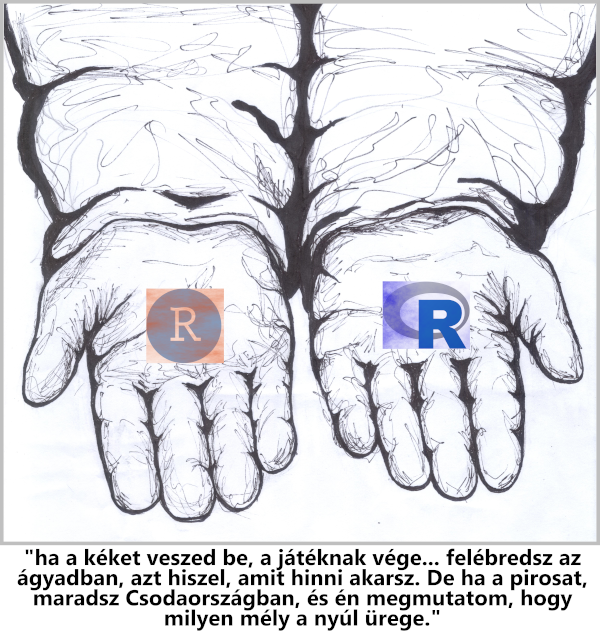
\includegraphics[width=0.7\linewidth]{images/ch_03_small} \end{center}

\hypertarget{a-fux151-komponensek-telepuxedtuxe9se}{%
\section{A fő komponensek telepítése}\label{a-fux151-komponensek-telepuxedtuxe9se}}

\begin{rmdlevel1}
Ebben a fejezetben:

\begin{itemize}
\tightlist
\item
  megismerjük az \emph{Alap R}, az \emph{RStudio} és a csomagok
  telepítését.
\end{itemize}
\end{rmdlevel1}

A korábbi fejezetekben megismertük az R világának néhány fogalmát és szereplőjét. Tudjuk, hogy az R nyelv használatához megfelelő szoftveres környezetre van szükség, amely magába foglalja az \emph{Alap R}-t és az \emph{egyéb csomagok} kategóriájából esetlegesen telepített csomagokat is. Az R már ezen eszközök birtokában is teljes körűen használható, azonban egy újabb ingyenes eszköz, az \emph{RStudio}, kényelmessé és hatékonnyá teszi az adatelemzési munkát.

Könyvünk legfontosabb gondolata: \textbf{ma akkor tudjuk a legjobban kihasználni az R lehetőségeit, és ezzel egyidőben a legkényelmesebb módon elvégezni az adatelemzési feladatunkat, ha (1) az \emph{Rstudio}-t használjuk, (2) projekt üzemmódban dolgozunk, és (3) RMarkdown állományokban rögzítjük az R parancsainkat.} Ezt a szemléletet következetesen képviseljük az egyes fejezetekben, és a későbbiekben részletesebben bemutatjuk, hogyan tudjuk mindezt megvalósítani.

A R kényelmes használatához a legelső lépés a szoftveres környezet egyes elemeinek telepítése. Három fő komponens telepítésére lesz szükségünk:

\begin{enumerate}
\def\labelenumi{\arabic{enumi}.}
\tightlist
\item
  \emph{Alap R}, amely tartalmazza a konzolt, az R interpretert, illetve a \emph{standard csomagokokat} és az \emph{ajánlott csomagokat},
\item
  \emph{RStudio}, amely egy új konzollal ``eltakarja'' az \emph{Alap R}-t, és kényelmesebb hozzáférést biztosít az \emph{Alap R} interpreteréhez és a csomagjaihoz.
\item
  Csomagok, amelyek az \emph{egyéb csomagok} nagy halmazából származnak, és telepítésükkel újabb és újabb képességekkel ruházzuk fel az \emph{Alap R}-t.
\end{enumerate}

\hypertarget{az-alap-r-telepuxedtuxe9se}{%
\subsection{Az Alap R telepítése}\label{az-alap-r-telepuxedtuxe9se}}

Az \emph{Alap R} telepítéséhez látogassunk el az R hivatalos letöltő oldalára: \emph{\url{https://cran.r-project.org/}}. Az operációs rendszerünknek megfelelő link kiválasztásával folytassuk a navigálást.

\begin{itemize}
\tightlist
\item
  A Windows felhasználók a \texttt{Download\ R\ for\ Windows} linken, majd a \texttt{base} linken kattintva jutnak el a telepítőprogram linkjéhez: \texttt{Download\ R\ X.X.X\ for\ Windows}. A sikeres letöltés után indítsuk el a telepítőt, és az alapértelmezetten felajánlott opciók nyugtázásával végezzük el a telepítést. A telepítést lehetőleg olyan Windows felhasználó alatt végezzük el, amelynek a neve sem ékezetes karaktert, sem szóközt, sem egyéb írásjelet nem tartalmaz.
\item
  A macOS felhasználók a \texttt{Download\ R\ for\ (Mac)\ OS\ X} linken kattintva jutnak a telepítőhöz: \texttt{R-X.X.X.pkg}. A letöltés után indítsuk el a telepítőt, és a \texttt{Next} gombok segítségével végezzük el a telepítést.
\item
  A Linux felhasználók az aktuális R verzió telepítéséhez a \texttt{Download\ R\ for\ Linux} linken keresztül jutnak el, ahol a megfelelő disztribúció (Debian, Redhat, Suse, Ubuntu) kiválasztása után konkrét információkat kapnak a telepítésről.
\end{itemize}

\hypertarget{az-rstudio-telepuxedtuxe9se}{%
\subsection{Az RStudio telepítése}\label{az-rstudio-telepuxedtuxe9se}}

Az \emph{RStudio} telepítéséhez az operációs rendszerünknek megfelelő telepítőt kell letöltenünk a \emph{\url{https://www.rstudio.com/products/rstudio/download/}} oldalról. Az RStudio Desktop (Open Source License) változatára lesz szükségünk, töltsük le és telepítsük ezt a számítógépünkre. A telepítés során fogadjuk el az alapértelmezett opciókat. Az \emph{RStudio} automatikusan megtalálja és használja a korábban telepített \emph{Alap R} példányunkat, így a későbbiekben elegendő lesz az \emph{RStudio}-t használni, azon keresztül elérhetjük az \emph{Alap R} minden funkcióját.

\hypertarget{Csomagoktelepitese}{%
\subsection{Csomagok telepítése}\label{Csomagoktelepitese}}

A csomagok telepítésére az \emph{Alap R} vagy az \emph{RStudio} elindítása után van módunk. Érdemes a telepítéseket az \emph{RStudio}-ból végezni. A csomag fellelési helye alapján, három különböző tárhelyről mutatjuk be a csomagok telepítését. Látni fogjuk, hogy a csomagok telepítéséhez R parancsokat fogunk használni. Ha még nem vagyunk jártasak R parancsok futtatásban, akkor a \ref{AzRStudiohasznalata} fejezet fellapozásával segítséget kaphatunk a lenti parancsok kipróbálásához, de úgy is eljárhatunk, hogy most kihagyjuk ennek a résznek az áttekintését, és később térünk vissza, amikor valóban felmerül az igény csomagok telepítésére.

Az R csomagok hivatalos helye a \href{https://cran.r-project.org/web/packages/}{CRAN (The Comprehensive R Archive Network)}. A CRAN számítógépei tárolják a nyílt forráskódú R nyelv és környezet különböző verzióinak kódjait és dokumentációit, így az összes R csomag forráskódját is. Egy bírálási folyamat után bármely felhasználó csomagja a CRAN-ból is elérhető lehet.

Az \emph{Alap R} vagy az \emph{RStudio} elindítása után az \texttt{install.packages()} függvénnyel tölthetünk le és telepíthetünk csomagot a CRAN-ról. Tetszőleges csomag telepítéséhez írjuk a csomag nevét idézőjelekben a függvény argumentumába:

\begin{Shaded}
\begin{Highlighting}[]
\NormalTok{install.packages("csomag\_neve")}
\end{Highlighting}
\end{Shaded}

A \textbf{psych} csomagot, amely a pszichológia kutatások adatainak elemzéséhez nyújt segítséget, például így telepíthetjük:

\begin{Shaded}
\begin{Highlighting}[]
\FunctionTok{install.packages}\NormalTok{(}\StringTok{"psych"}\NormalTok{)        }\CommentTok{\# psych csomag telepítése}
\end{Highlighting}
\end{Shaded}

A csomagok másik fontos forrása a \href{https://www.bioconductor.org/}{Bioconductor}, ahol alaposan tesztelt és igen jól dokumentált bioinformatikai témájú csomagokat találunk. Az innen elérhető csomagokat -- például most a \textbf{DESeq2} csomagot az RNS-szekvenálási elemzésekhez -- a következő parancsokkal telepíthetjük:

\begin{Shaded}
\begin{Highlighting}[]
\ControlFlowTok{if}\NormalTok{ (}\SpecialCharTok{!}\FunctionTok{requireNamespace}\NormalTok{(}\StringTok{"BiocManager"}\NormalTok{, }\AttributeTok{quietly =} \ConstantTok{TRUE}\NormalTok{))}
    \FunctionTok{install.packages}\NormalTok{(}\StringTok{"BiocManager"}\NormalTok{)}
\NormalTok{BiocManager}\SpecialCharTok{::}\FunctionTok{install}\NormalTok{(}\StringTok{"DESeq2"}\NormalTok{)}
\end{Highlighting}
\end{Shaded}

A csomagok harmadik fő forrása a GitHub. A felhasználók a saját fejlesztésű csomagjaikat rendszerint először a GitHub-on keresztül teszik elérhetővé. Ha ezeket a csomagokat szeretnénk kipróbálni, akkor a felhasználó és a csomag nevének birtokában a következő parancsot kell kiadnunk:

\begin{verbatim}
devtools::install_github("felhasznalo_neve/csomag_neve")
\end{verbatim}

Például a GitHub-ról telepíthető \textbf{emo} csomag segítségvel hangulatjeleket szúrhatunk be az RMarkdown állományainkba. Ezzel a sorral telepíthetjük a csomagot:

\begin{Shaded}
\begin{Highlighting}[]
\NormalTok{devtools}\SpecialCharTok{::}\FunctionTok{install\_github}\NormalTok{(}\StringTok{"hadley/emo"}\NormalTok{)}
\end{Highlighting}
\end{Shaded}

Fontos tudnunk, hogy a csomagok telepítésére egy számítógépen egy adott R verzión belül csak egyszer van szükség. A telepítő parancsainkat azonban érdemes megőrizni, hogy ha szükséges, akkor egy új R verzióban könnyen tudjuk telepíteni a korábban használt csomagjainkat. Nagyon fontos, hogy a telepítő parancsok futtatása után, tegyük azokat megjegyzésbe, vagyis írjunk előjük kettőskereszt (\texttt{\#}) karaktert (részletesebb információkat a megjegyzésekről a \ref{MegjegyzesazRben} fejezetben olvashatunk). Ezzel tudjuk megvédeni ezeket a telepítő parancsokat az újbóli, véletlen, felesleges végrehajtástól. Ennek megfelelően a telepítő parancsainkat ilyen formában kell őriznünk:

\begin{Shaded}
\begin{Highlighting}[]
\CommentTok{\# install.packages("psych")        \# psych csomag telepítése}
\CommentTok{\# if (!requireNamespace("BiocManager", quietly = TRUE))}
\CommentTok{\#     install.packages("BiocManager")}
\CommentTok{\# BiocManager::install("DESeq2")}
\CommentTok{\# devtools::install\_github("hadley/emo")}
\end{Highlighting}
\end{Shaded}

Vegyük figyelmbe, hogy egy csomag telepítése során más, egyéb csomagok telepítése automatikusan is megtörténhet, tehát egy helyett valójában több csomag is felkerülhet a gépünkre. Az is előfordulhat, hogy egy csomag telepítése csak akkor lesz sikeres, ha más csomagok frissítését engedélyezzük az adott csomag telepítése során. Végül előfordulhat olyan eset is, amikor egy csomag telepítése valamilyen oknál fogva meghiúsul. Erról minden esetben hibaüzenet tájékoztat minket, és ez szinte minden esetben jó kiindulásul szolgál a hibát okozó körülmény elhárításában. A legtöbbször egy másik csomag hiánya okozza a sikertelen telepítést, ezért olvassuk ki a hibaüzenetből a hiányolt csomag nevét, és először ennek a telepítését végezzük el.

\begin{rmdsummary}
\textbf{Összefoglalás}

Az R kényelmes használatához először telepítsük az operációs
rendszerünknek megfelelő \emph{Alap R}, majd az \emph{RStudio} legújabb
verzióját. Az R képességeit csomagok segítségével bővíthetjük, ehhez
legtöbbször az \texttt{install.packages()} parancsot használjuk.
\end{rmdsummary}

\begin{rmdexercise}
\textbf{Feladatok}

\begin{enumerate}
\def\labelenumi{\arabic{enumi}.}
\tightlist
\item
  Melyik az R legfrissebb változata, és milyen újdonságokat tartalmaz az előző változathoz képest?
\item
  Melyik az \emph{RStudio} legfrissebb változata, és milyen újdonságokat tartalmaz az előző változathoz képest?
\item
  Hogyan deríthető ki, hogy egy csomagban (például a \textbf{MASS}) csomagban, hány adatobjektum, és hány függvény található?
\end{enumerate}
\end{rmdexercise}

\hypertarget{a-tidyverse-r-telepuxedtuxe9se}{%
\section{A Tidyverse R telepítése}\label{a-tidyverse-r-telepuxedtuxe9se}}

\begin{rmdlevel2}
Ebben a fejezetben:

\begin{itemize}
\tightlist
\item
  megismerjük a \emph{Tidyverse R} telepítését.
\end{itemize}
\end{rmdlevel2}

A \emph{Tidyverse R} az R meglévő funkcióinak új szemléletű használatát jelenti. A modern R jelenleg egyet jelent a \emph{Tidyverse R}-rel, az ebben a szemléleteben készült parancsaink gyorsak, jól olvashatók és könnyen módosíthatók. A \emph{Tidyverse R} funkciói összesen 8 csomagba (\textbf{ggplot2}, \textbf{purrr}, \textbf{tibble}, \textbf{dplyr}, \textbf{tidyr}, \textbf{stringr}, \textbf{readr} és \textbf{forcats}) vannak szétosztva, mindegyik csomag egy-egy témakört fed le. A fenti csomagok telepítése egyetlen gyűjtőcsomag a \textbf{tidyverse} nevű csomag telepítésével is elvégezhető:

\begin{Shaded}
\begin{Highlighting}[]
\FunctionTok{install.packages}\NormalTok{(}\StringTok{"tidyverse"}\NormalTok{) }\CommentTok{\# a Tidyverse R telepítése}
\end{Highlighting}
\end{Shaded}

A \emph{Tidyverse R} telepítését követően a csomagokban lévő függvények használatához a \emph{Tidyverse R} betöltésére is szükség van. Hívjuk meg a \texttt{library()} függvényt, amely ebben az esetben igen részletes tájékoztatást ad az újonnan elérhető csomagokról.

\begin{Shaded}
\begin{Highlighting}[]
\FunctionTok{library}\NormalTok{(tidyverse)}
\CommentTok{\#\textgreater{} {-}{-} Attaching packages {-}{-}{-}{-}{-}{-}{-}{-}{-}{-}{-}{-}{-}{-}{-}{-}{-}{-}{-}{-}{-}{-}{-}{-}{-}{-}{-}{-}{-} tidyverse 1.3.0 {-}{-}}
\CommentTok{\#\textgreater{} \textless{}U+221A\textgreater{} ggplot2 3.3.0     \textless{}U+221A\textgreater{} purrr   0.3.3}
\CommentTok{\#\textgreater{} \textless{}U+221A\textgreater{} tibble  3.0.0     \textless{}U+221A\textgreater{} dplyr   0.8.5}
\CommentTok{\#\textgreater{} \textless{}U+221A\textgreater{} tidyr   1.0.2     \textless{}U+221A\textgreater{} stringr 1.4.0}
\CommentTok{\#\textgreater{} \textless{}U+221A\textgreater{} readr   1.3.1     \textless{}U+221A\textgreater{} forcats 0.5.0}
\CommentTok{\#\textgreater{} {-}{-} Conflicts {-}{-}{-}{-}{-}{-}{-}{-}{-}{-}{-}{-}{-}{-}{-}{-}{-}{-}{-}{-}{-}{-}{-}{-}{-}{-}{-}{-}{-}{-}{-}{-} tidyverse\_conflicts() {-}{-}}
\CommentTok{\#\textgreater{} x dplyr::filter() masks stats::filter()}
\CommentTok{\#\textgreater{} x dplyr::lag()    masks stats::lag()}
\end{Highlighting}
\end{Shaded}

A \emph{Tidyverse R} csomagjait jelenleg is intenzíven fejlesztik, így gyakran jelenik meg újabb és újabb verzió. Érdemes ellenőrizni, hogy a \emph{Tidyverse R} csomagjai közül a legfrissebbeket használjuk-e. Ehhez a \textbf{tidyverse} csomag \texttt{tidyverse\_update()} függvényét használjuk.

\begin{Shaded}
\begin{Highlighting}[]
\NormalTok{tidyverse}\SpecialCharTok{::}\FunctionTok{tidyverse\_update}\NormalTok{()}
\CommentTok{\#\textgreater{} The following packages are out of date:}
\CommentTok{\#\textgreater{} }
\CommentTok{\#\textgreater{} * lubridate (1.7.4 {-}\textgreater{} 1.7.8)}
\CommentTok{\#\textgreater{} * purrr     (0.3.3 {-}\textgreater{} 0.3.4)}
\CommentTok{\#\textgreater{} * xml2      (1.2.5 {-}\textgreater{} 1.3.1)}
\CommentTok{\#\textgreater{} }
\CommentTok{\#\textgreater{} Start a clean R session then run:}
\CommentTok{\#\textgreater{} install.packages(c("lubridate", "purrr", "xml2"))}
\end{Highlighting}
\end{Shaded}

Például a fenti esetben 3 csomag frissítését javasolja a \texttt{tidyverse\_update()} függvény, és segítséget is ad a telepítőparancs listázásával.

\begin{rmdsummary}
\textbf{Összefoglalás}

A \emph{Tidyverse R} használatához elegendő telepítenünk a
\textbf{tidyverse} csomagot, amely a többi 8 csomag telepítését
automatikusan elvégzi. A telepítést a
\texttt{install.packages("tidyverse")} paranccsal végezzük. Időnként
ellenőrizzük a \texttt{tidyverse::tidyverse\_update()} segítségével,
hogy a legfrissebb változatát használjuk-e a \emph{Tidyverse R}-t alkotó
csomagoknak.
\end{rmdsummary}

\begin{rmdexercise}
\textbf{Feladatok}

\begin{enumerate}
\def\labelenumi{\arabic{enumi}.}
\tightlist
\item
  Keressünk rá a \emph{Tidyverse R} csomagjaira, és próbáljuk kideríteni az egyes csomagok fő célját, alkalmazási területeit!
\item
  Derítsük ki, hogy az R Core Team vagy Hadley Wickham több R csomag szerzője!
\end{enumerate}
\end{rmdexercise}

\hypertarget{az-r-frissuxedtuxe9se}{%
\section{Az R frissítése}\label{az-r-frissuxedtuxe9se}}

\begin{rmdlevel3}
Ebben a fejezetben:

\begin{itemize}
\tightlist
\item
  bemutatjuk az \emph{Alap R}, az \emph{RStudio} és a csomagok
  frissítését.
\end{itemize}
\end{rmdlevel3}

A R ideális használata során az \emph{RStudio}-ban dolgozunk, és így érjük el az \emph{Alap R} és az egyes csomagok szolgáltatásait. A mai napig mindhárom komponenst intenzíven fejlesztik, újabb és újabb funkciókat építenek be, és az esetleges hibákat rendre javítják a frissebb változatokban. Az \emph{Alap R} évente kb. négyszer frissül, az \emph{RStudio} háromszor, és érdemes időnként azt is ellenőrizni, hogy a gyakran használt csomagjainkból nincs-e frissebb példány.

\hypertarget{az-alap-r-frissuxedtuxe9se}{%
\subsection{Az Alap R frissítése}\label{az-alap-r-frissuxedtuxe9se}}

A telepített \emph{Alap R} verzióját az \texttt{R.version.string} végrehajtásával ellenőrizhetjük. Amennyiben az R hivatalos \href{https://cran.r-project.org/}{oldalán} találunk frissebb példányt, akkor legalább két módszer segítségével frissíthetjük az \emph{Alap R}-t. Megjegyezzük, hogy az \emph{Alap R} sikeres frissítése után az \emph{RStudio} automatikusan az új példányt fogja használni.

\textbf{1. módszer: csak Windows alatt.} Windows operációs rendszer alatt rendelkezésre áll az \textbf{installr} csomag, amelynek pontosan az a feladata, hogy kényelmesen telepíthessük számítógépünkre az R legfrissebb verzióját. Az \textbf{installr} a régebbi verzióban lévő csomagokat az új változatba is átmozgatja, és ott azok frissítését is elvégzi. A következő parancsok futtatására van szükség.

\begin{Shaded}
\begin{Highlighting}[]
\CommentTok{\# install.packages("installr") \# az installr csomag telepítése}
\FunctionTok{library}\NormalTok{(installr)              }\CommentTok{\# az installr csomag betöltése}
\FunctionTok{updateR}\NormalTok{()                      }\CommentTok{\# az Alap R és a csomagok frissítése}
\end{Highlighting}
\end{Shaded}

\textbf{2. módszer: általános út.} Az \emph{Alap R} frissítésének másik módja, hogy telepítünk egy új példányt a régi R mellé. Azaz a korábban látott módon letöltjük és telepítjük az \emph{Alap R} legújabb változatát, pontosan úgy, mintha még nem lenne a gépünkön működő R. Ez az új verzió azonban félkarú óriás mindaddig, amíg a régi R verzióban használt összes csomagot nem telepítjük újra az új verzióban is. Ezt magunk egyesével is megtehetjük, ha korábban összegyűjtöttük a csomagtelepítő parancsainkat, legyen szó akár akár a CRAN, a Bioconductor vagy a GitHub oldaláról származó csomagokról. Ha ezek nem állnak rendelkezésre, akkor az \emph{Alap R} frissítésének általános útját három lépésben foglalhatjuk össze.

\begin{enumerate}
\def\labelenumi{\arabic{enumi}.}
\tightlist
\item
  Indítsuk el az \emph{RStudio}-t még az új R verzió telepítése előtt, és futtassuk le a következő sorokat. A futtatás eredménye egy bináris állomány (\texttt{csomagok.rds}), amely a régi R összes telepített csomagjának nevét és más információkat tartalmaz. Lépjünk ki az \emph{RStudio}-ból.
\end{enumerate}

\begin{Shaded}
\begin{Highlighting}[]
\NormalTok{telepitett.csomagok }\OtherTok{\textless{}{-}} \FunctionTok{installed.packages}\NormalTok{(}\AttributeTok{priority=}\StringTok{"NA"}\NormalTok{)}
\FunctionTok{saveRDS}\NormalTok{(}\AttributeTok{object =}\NormalTok{ telepitett.csomagok, }\AttributeTok{file =} \StringTok{"csomagok.rds"}\NormalTok{)}
\end{Highlighting}
\end{Shaded}

\begin{enumerate}
\def\labelenumi{\arabic{enumi}.}
\setcounter{enumi}{1}
\item
  Telepítsük az \emph{Alap R} új verzióját.
\item
  Indítsuk el az \emph{RStudio}-t és futtassuk le a lenti sorokat. A folyamat több percig is eltarthat. Az \emph{RStudio} már az új R verziót használja, így a csomagok az új R tudását egészítik ki.
\end{enumerate}

\begin{Shaded}
\begin{Highlighting}[]
\NormalTok{telepitett.csomagok }\OtherTok{\textless{}{-}} \FunctionTok{readRDS}\NormalTok{(}\AttributeTok{file =} \StringTok{"csomagok.rds"}\NormalTok{)}
\FunctionTok{install.packages}\NormalTok{(}\AttributeTok{pkgs=}\NormalTok{telepitett.csomagok[,}\DecValTok{1}\NormalTok{])}
\end{Highlighting}
\end{Shaded}

Megjegyezzük, hogy a fenti 2. módszer segítségével csak a CRAN csomagjait tudjuk telepíteni, a Bioconductor és a GitHub oldalakról származó csomagok telepítését magunknak kell megismételni.

\hypertarget{az-rstudio-frissuxedtuxe9se}{%
\subsection{Az RStudio frissítése}\label{az-rstudio-frissuxedtuxe9se}}

A telepített \emph{RStudio} példányunk verziószámát a \texttt{Help\ /\ About\ RStudio} menüpont segítségével, vagy az \texttt{rstudioapi::versionInfo()} parancs futtatásával ellenőrizhetjük. Frissebb verzió létezéséről a \texttt{Help\ /\ Check\ for\ Updates} menüpont ad tájékoztatást. Amennyiben találunk újabb verziót az \emph{RStudio} hivatalos \href{https://rstudio.com/}{honlapján}, töltsük le az operációs rendszerünknek megfelelő változatot és indítsuk el a telepítőt. Szerencsére a régi \emph{RStudio} beállításait örökli az új példány.

\hypertarget{csomagok-frissuxedtuxe9se}{%
\subsection{Csomagok frissítése}\label{csomagok-frissuxedtuxe9se}}

A korábban telepített csomagokat az \emph{RStudio} \texttt{Tools/Check\ for\ Package\ Updates} menüpontjával frissíthetjük. A frissíthető csomagok megjelennek egy dialógus dobozban, jelöljük ki az összes csomagot és indítsuk el a telepítési folyamatot. A következő R parancs végrehajtásával is frissíthetjük a csomagjainkat.

\begin{Shaded}
\begin{Highlighting}[]
\FunctionTok{update.packages}\NormalTok{(}\AttributeTok{ask=}\ConstantTok{FALSE}\NormalTok{) }
\end{Highlighting}
\end{Shaded}

\begin{rmdsummary}
\textbf{Összefoglalás}

Az \emph{Alap R}, az \emph{RStudio} és az egyes csomagok időről-időre
megújulnak, érdemes évente legalább egy-két alkalommal elvégezni ezek
frissítését. Az \emph{Alap R} frissítése lényegében egy új verzió
telepítését jelenti, a régi R továbbra is elérhető marad. Az
\emph{RStudio} frissítése után csak az új verziót használhatjuk. Az
\emph{Alap R} és az \emph{RStudio} friss verziója a hivatalos
honlapokról szerezhető be. A csomagok frissítéséhez használjuk a
\texttt{update.packages(ask=FALSE)} parancsot.
\end{rmdsummary}

\begin{rmdexercise}
\textbf{Feladatok}

\begin{enumerate}
\def\labelenumi{\arabic{enumi}.}
\tightlist
\item
  Az \emph{RStudio} \texttt{Tools/Check\ for\ Package\ Updates} menüpontjával tájékozódjunk a telepített csomagjaink állapotáról. Végezzük el a szükséges frissítéseket!
\end{enumerate}
\end{rmdexercise}

\hypertarget{munka-az-r-ben}{%
\chapter{Munka az R-ben}\label{munka-az-r-ben}}

\begin{center}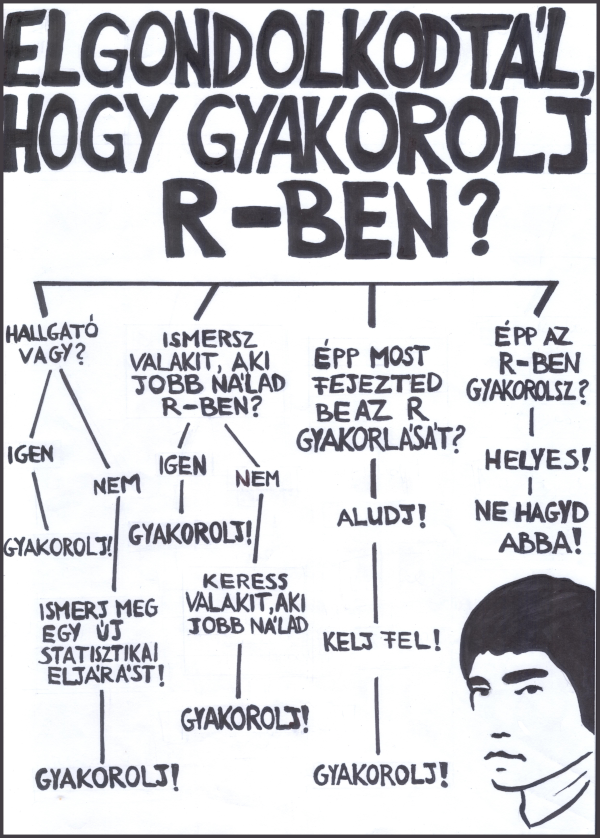
\includegraphics[width=0.7\linewidth]{images/ch_04_small} \end{center}

\hypertarget{AzRStudiohasznalata}{%
\section{Az RStudio használata}\label{AzRStudiohasznalata}}

\begin{rmdlevel1}
Ebben a fejezetben:

\begin{itemize}
\tightlist
\item
  megismerjük az \emph{RStudio} jellemzőit és felépítését,
\item
  a konzolos és parancsállományos használat különbségeit,
\item
  a parancsállományok és az RMarkdown állományok lehetőségeit,
\item
  a projekt fogalmát és használatát,
\item
  és az \emph{RStudio} billenytűparancsait.
\end{itemize}
\end{rmdlevel1}

\hypertarget{az-r-nyelv}{%
\chapter{Az R nyelv}\label{az-r-nyelv}}

\begin{center}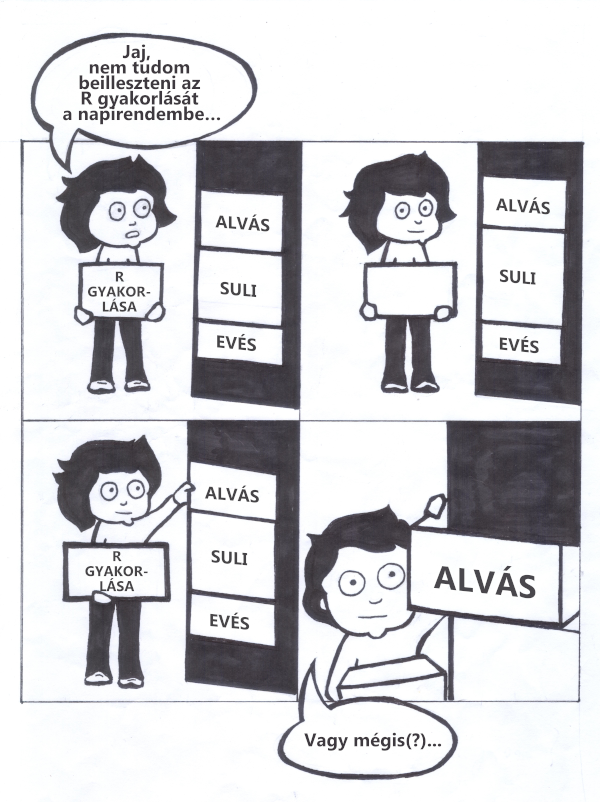
\includegraphics[width=0.7\linewidth]{images/ch_05_small} \end{center}

Az előző fejezetekben megismertük az R környezetet, az \emph{Alap R}, az \emph{RStudio} és a csomagok telepítését, megtanultuk a projektek, parancsállományok és RMarkdown állományok létrehozását. Tudjuk, a különböző környezetekben eltérő módszerekkel hajthatjuk végre az R parancsokat: a konzolban az \texttt{ENTER}, a Windows-os \emph{RGui}-ban a \texttt{Ctrl+R}, míg az \emph{RStudio}-ban a \texttt{Ctrl+Enter} billentyűkombinációt kell használnunk. A parancsok végrehajtása közben érdemes észben tartani, ha a folytatás prompt (\texttt{+}) feltűnik, akkor kattintsunk bele a konzolba, és nyomjuk meg az \texttt{Esc} billentyűt, így tudunk kilépni a befejezetlen sor szerkesztéséből

A fejezet példáinak kipróbáláshoz hozzunk létre egy \texttt{gyakorlas} nevű új projektet az \emph{RStudio}-ban (\texttt{File\ /\ New\ Project}), majd készítsünk egy \texttt{gyakorlas.Rmd} RMarkdown állományt (\texttt{File\ /\ New\ File\ /\ R\ Markdown}) és egy \texttt{gyakorlas.R} parancsállományt (\texttt{File\ /\ New\ File\ /\ R\ Script}). A fejezet példáit felváltva gépeljük az RMarkdown állomány R csonkjaiba, illetve a parancsállomány tetszőleges soraiba. A fejezet további részében az R nyelvre koncentrálunk, arra, hogy mit írunk, és nem arra, hogy hová írjuk a parancsokat.

\hypertarget{adatobjektumok}{%
\section{Adatobjektumok}\label{adatobjektumok}}

\begin{rmdlevel1}
Ebben a fejezetben:

\begin{itemize}
\tightlist
\item
  áttekintjük az egyszerű számolási lehetőségek R-ben,
\item
  bevezetjük az aritmetikai operátor és a kifejezés fogalmát,
\item
  megismerjük az objektum létrehozását és elnevezését,
\item
  több parancs elhelyezését egy sorban,
\item
  és a megjegyzések használatát.
\end{itemize}
\end{rmdlevel1}

\hypertarget{beolvasas}{%
\chapter{Beolvasás}\label{beolvasas}}

\begin{center}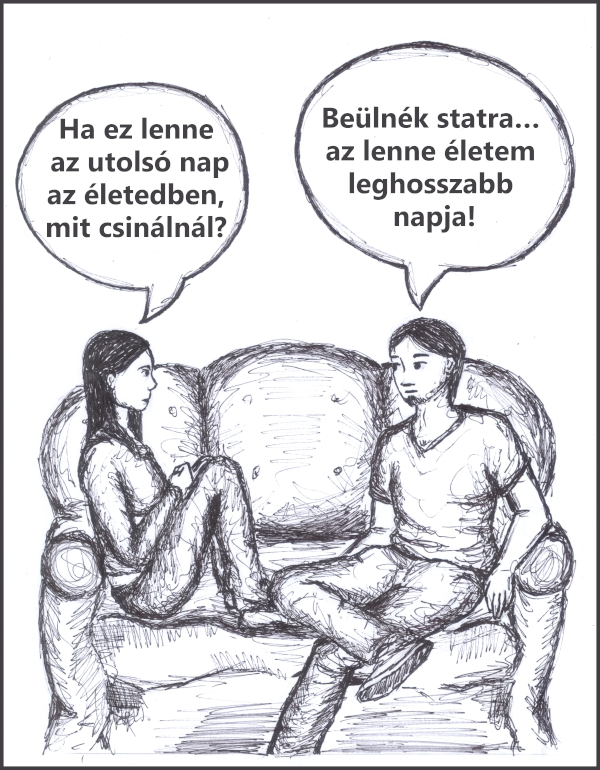
\includegraphics[width=0.7\linewidth]{images/ch_06_small} \end{center}

\hypertarget{beolvas-kiir}{%
\section{Alapvető formátumok}\label{beolvas-kiir}}

\begin{rmdlevel1}
Ebben a fejezetben áttekintjük:

\begin{itemize}
\tightlist
\item
  mit nevezünk tagolt szöveges állománynak, hogyan hozzuk létre
\item
  inline és állományos beolvasás közötti különbség
\item
  az inline beolvasás esetei
\item
  tagolt szöveges állomány beolvasása és kiírása (AR és TR)
\item
  fix széles mezővel rendelkező állományok olvasása
\item
  más statisztikai programcsomagok adatállományainak olvasása és írása
\item
  objektumok írása és olvasása bináris állományba
\end{itemize}
\end{rmdlevel1}

\hypertarget{adatmanipulacio}{%
\chapter{Adatmanipuláció}\label{adatmanipulacio}}

\begin{center}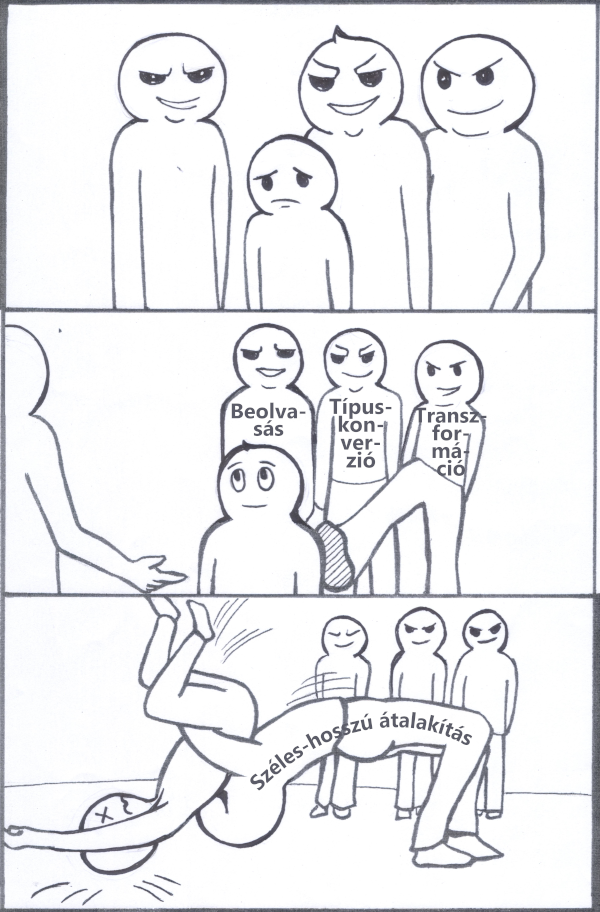
\includegraphics[width=0.7\linewidth]{images/ch_07_small} \end{center}

\hypertarget{adatkezeluxe9s-az-alap-r-ben}{%
\section{Adatkezelés az Alap R-ben}\label{adatkezeluxe9s-az-alap-r-ben}}

\begin{rmdlevel1}
Ebben a fejezetben:
\end{rmdlevel1}

\hypertarget{leiro-statisztika}{%
\chapter{Leíró statisztika}\label{leiro-statisztika}}

\begin{center}
\includegraphics[width=0.7\linewidth]{images/ch_08_small} \end{center}

\begin{rmdlevel1}
Ebben a fejezetben áttekintjük:
\end{rmdlevel1}

\hypertarget{grafika-az-r-ben}{%
\chapter{Grafika az R-ben}\label{grafika-az-r-ben}}

\begin{center}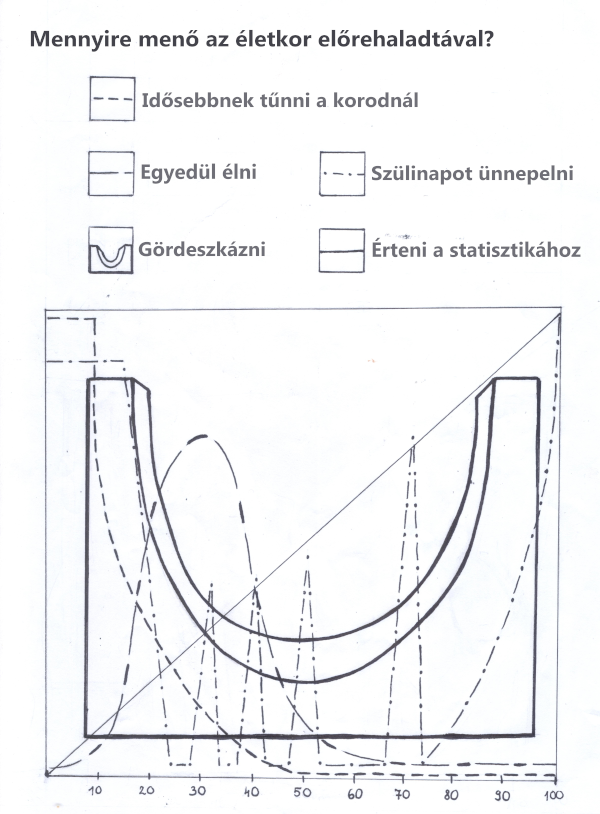
\includegraphics[width=0.7\linewidth]{images/ch_09_small} \end{center}

\begin{rmdlevel1}
Ebben a fejezetben áttekintjük:

\begin{itemize}
\tightlist
\item
  az R grafikus rendszerei
\item
  a hagyományos grafika alapfogalmai
\item
  magasszintű és alacsonyszintű rajzfüggvények a hagyományos grafikában
\item
  a ggplot2 rendszer alapelve
\item
  ábrák létrehozása ggplot2-ben
\item
  ábrák mentése háttértárra
\end{itemize}
\end{rmdlevel1}

\hypertarget{hipotezisvizsgalatok}{%
\chapter{Hipotézisvizsgálatok}\label{hipotezisvizsgalatok}}

\begin{center}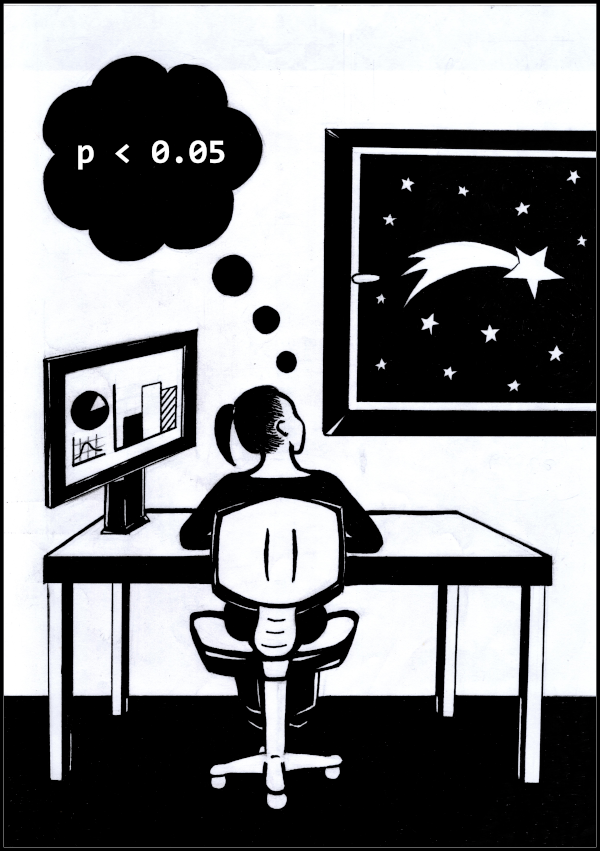
\includegraphics[width=0.7\linewidth]{images/ch_10_small} \end{center}

\begin{rmdlevel1}
Ebben a fejezetben a statisztika azon klasszikus próbáit foglaltuk össze, amelyek jellemzően egy- vagy kétmintás hipotézisvizsgálatokat jelentenek. Az öt alfejezet a nullhipotézisben szereplő állításoknak és paramétereknek megfelelően a statisztikai próbák különböző csoportjait fedi le:

\begin{itemize}
\tightlist
\item
  várható értékre vonatkozó próbák
\item
  mediánra vonatkozó nemparaméteres próbák
\item
  valószínűségre vonatkozó próbák
\item
  varianciára vonatkozó próbák
\item
  az eloszlás egészére vonatkozó próbák.
\end{itemize}
\end{rmdlevel1}

\hypertarget{publikacio}{%
\chapter{Publikáció}\label{publikacio}}

\begin{center}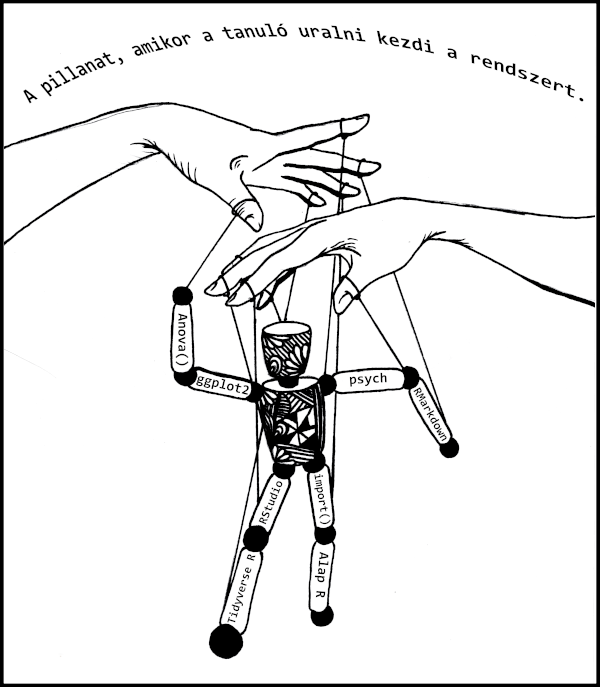
\includegraphics[width=0.7\linewidth]{images/ch_11_small} \end{center}

\hypertarget{reprodukuxe1lhatuxf3-kutatuxe1s}{%
\section{Reprodukálható kutatás}\label{reprodukuxe1lhatuxf3-kutatuxe1s}}

A kutatás és oktatás világában jelentős elmozdulás figyelhető meg a reprodukálható kutatás felé.

igénye felé. „Az akadémiai kutatás végső terméke a papír, a laboratóriumi jegyzetfüzetekkel és a teljes számítási környezettel együtt az eredmények előállítása érdekében, mint például a kód, az adatok stb., Amelyek felhasználhatók az eredmények reprodukálására és új munka létrehozására a kutatás ''(Wikipedia).

Ennek következménye az, hogy meg kell változtatnunk szokásainkat, és minden kéziratunkat, előadásainkat, házi feladatainkat stb. Tiszta és reprodukálható formában kell elkezdenünk, azaz ha valaki megadja a kódot, akkor ez a személy pontosan reprodukálhatja a dokumentumot. Ez a dokumentum megkönnyíti ezt az átmenetet az R Markdown segítségével.

\hypertarget{appendix-fuxfcggeluxe9k}{%
\appendix}


\hypertarget{megoldasok}{%
\chapter{Megoldások}\label{megoldasok}}

\hypertarget{itt-kezdodik-1-exercise-solution}{%
\section{Megoldások az \ref{itt-kezdodik-1-exercise} feladatokhoz}\label{itt-kezdodik-1-exercise-solution}}

\begin{quote}
\begin{enumerate}
\def\labelenumi{\arabic{enumi}.}
\tightlist
\item
  Milyen online vagy nyomtat könyvek segítik az R elsajátítását? Próbáljuk összegyűjteni a magyar nyelvű könyveket is!
\end{enumerate}
\end{quote}

Az R könyvekkel kapcsolatban könnyen az lehet az érzésünk, hogy \emph{túl sok a könyv, és túl kevés az idő}. Valóban tengernyi R könyv vásárolható meg, melyek többsége angol nyelvű. Elegendő a Springer \href{https://www.springer.com/series/6991}{Use R!} könyvsorozatára gondolni, amely önmagában több mint 80 címet tartalmaz. Az Amazon-ról elérhető, 2020. januárja után \href{https://www.amazon.com/s?k=r+statistics\&i=stripbooks\&rh=n\%3A5\&s=relevanceexprank\&Adv-Srch-Books-Submit.x=39\&Adv-Srch-Books-Submit.y=5\&field-datemod=1\&field-dateop=After\&field-dateyear=2020\&unfiltered=1\&ref=sr_adv_b}{megjelent} könyvek száma is túl van a kétszázon.

Különösen értékesek lehetnek az online elérhető könyvek. Az idegen nyelvű könyvek tematikus gyűjteménye a \href{https://www.bigbookofr.com/}{Big Book of R}, míg az R erőforrásokról \href{https://abarik.github.io/roforrasok/}{saját listát} is karbantartok.

A magyar nyelvű könyvek közül külön is felsorolunk néhányat:

\begin{itemize}
\tightlist
\item
  Reiczigel Jenő, Harnos Andrea, Solymosi Norbert (2021). \emph{Biostatisztika nem statisztikusoknak}. Pars Kft., Nagykovácsi.
\item
  Dinya Elek, Solymosi Norbert (2016). \emph{Biometria a klinikumban 2. Feladatok megoldása R-környezetben.} Medicina Kiadó.
\item
  Münnich Ákos, Nagy Ágnes, Abari Kálmán. \emph{Többváltozós statisztika pszichológus hallgatók számára.} Bölcsész Konzorcium, Debrecen, 2006. (\url{http://psycho.unideb.hu/statisztika})
  ISBN 963 9704 04 0
\end{itemize}

\begin{quote}
\begin{enumerate}
\def\labelenumi{\arabic{enumi}.}
\setcounter{enumi}{1}
\tightlist
\item
  Térképezzük fel az online videókurzusokat is az R tanulásához!
\end{enumerate}
\end{quote}

A videókurzusok többsége is angol nyelvű, a \href{https://www.youtube.com/results?search_query=r+statistics}{Youtube}-ról ingyenesen, de a \href{https://www.udemy.com/}{Udemy} vagy a \href{https://www.datacamp.com/}{datacamp} oldaláról előfizetés ellenében több száz kurzust is elérhetünk.

Az R-rel való ismerkedést kezdhetjük az \href{https://www.youtube.com/playlist?list=PLnmeQHnHYqv6ENGrdTXiE9YJrvHuxH2C9}{R a gyakorlatban} videósorozatommal is.

\begin{quote}
\begin{enumerate}
\def\labelenumi{\arabic{enumi}.}
\setcounter{enumi}{2}
\tightlist
\item
  A bevezető példa (\emph{Két tanítási módszer összehasonlítása}) megoldásában a hipotézisvizsgálat alapján adjunk szöveges értékelést!
\end{enumerate}
\end{quote}

A Mann-Whitney-próba alapján azt mondhatjuk, elegendő bizonyítékot találtunk arra, hogy a modern (Sprego) módszer eredményesebb (Mdn=0,36), mint a hagyományos (Mdn=0,66) tanítási módszer (W=24; p=0,001).

\hypertarget{szinek}{%
\chapter{Színek}\label{szinek}}

Az R grafikus elemeinek a színét magunk is megválaszthatjuk. Ehhez nyújt segítséget ez a függelék.

Megismerjük

\begin{itemize}
\tightlist
\item
  az előre definiált paletta színeit (\ref{az-elore-definialt} fejezet),
\item
  színek választását az \textbf{RColorBrewer} csomag segítségével (\ref{szinek-valasztasa-rcolorbrewer} fejezet),
\item
  színek választása a \textbf{dichromat} csomag segítségével (\ref{szinek-valasztasa-dichromat} fejezet),
\item
  színek választását egyéb paletták segítségével (\ref{szinek-valasztasa-egyeb} fejezet),
\item
  és végül az előre definiált 657 színnevet (\ref{a-657-szinnev} fejezet).
\end{itemize}

\hypertarget{az-elore-definialt}{%
\section{Az előre definiált paletta színei}\label{az-elore-definialt}}

Az előre definiált paletta 8 színt tartalmaz. A \ref{fig:default-palette} ábra az alapértelmezett színeket tartalmazza. Az előre definiált paletta egyes színeit sorszámokkal (1, 2 stb.) tudjuk elérni, amelyeket rendszerint a rajzfüggvények \texttt{col=} argumentumában kell elhelyezni. Az 1. szín a palettán a fekete, a második a piros, és így tovább.

\begin{Shaded}
\begin{Highlighting}[]
\FunctionTok{set.seed}\NormalTok{(}\DecValTok{0}\NormalTok{)}
\NormalTok{x }\OtherTok{\textless{}{-}} \FunctionTok{rpois}\NormalTok{(}\AttributeTok{n =} \DecValTok{50}\NormalTok{, }\AttributeTok{lambda =} \DecValTok{100}\NormalTok{)}
\FunctionTok{par}\NormalTok{(}\AttributeTok{las =} \DecValTok{1}\NormalTok{, }\AttributeTok{mgp =} \FunctionTok{c}\NormalTok{(}\DecValTok{0}\NormalTok{, }\FloatTok{0.2}\NormalTok{, }\DecValTok{0}\NormalTok{), }\AttributeTok{tcl =} \SpecialCharTok{{-}}\FloatTok{0.2}\NormalTok{, }\AttributeTok{mar =} \FunctionTok{c}\NormalTok{(}\DecValTok{3}\NormalTok{, }\DecValTok{2}\NormalTok{, }\DecValTok{1}\NormalTok{, }\DecValTok{1}\NormalTok{))}
\NormalTok{bar }\OtherTok{\textless{}{-}} \FunctionTok{barplot}\NormalTok{(x[}\DecValTok{1}\SpecialCharTok{:}\DecValTok{8}\NormalTok{], }\AttributeTok{col =} \DecValTok{1}\SpecialCharTok{:}\DecValTok{8}\NormalTok{, }\AttributeTok{names.arg =} \DecValTok{1}\SpecialCharTok{:}\DecValTok{8}\NormalTok{)}
\FunctionTok{mtext}\NormalTok{(}\AttributeTok{side =} \DecValTok{1}\NormalTok{, }\AttributeTok{at =}\NormalTok{ bar, }\AttributeTok{text =} \FunctionTok{palette}\NormalTok{(), }\AttributeTok{line =} \DecValTok{1}\NormalTok{)}
\end{Highlighting}
\end{Shaded}

\begin{figure}

{\centering 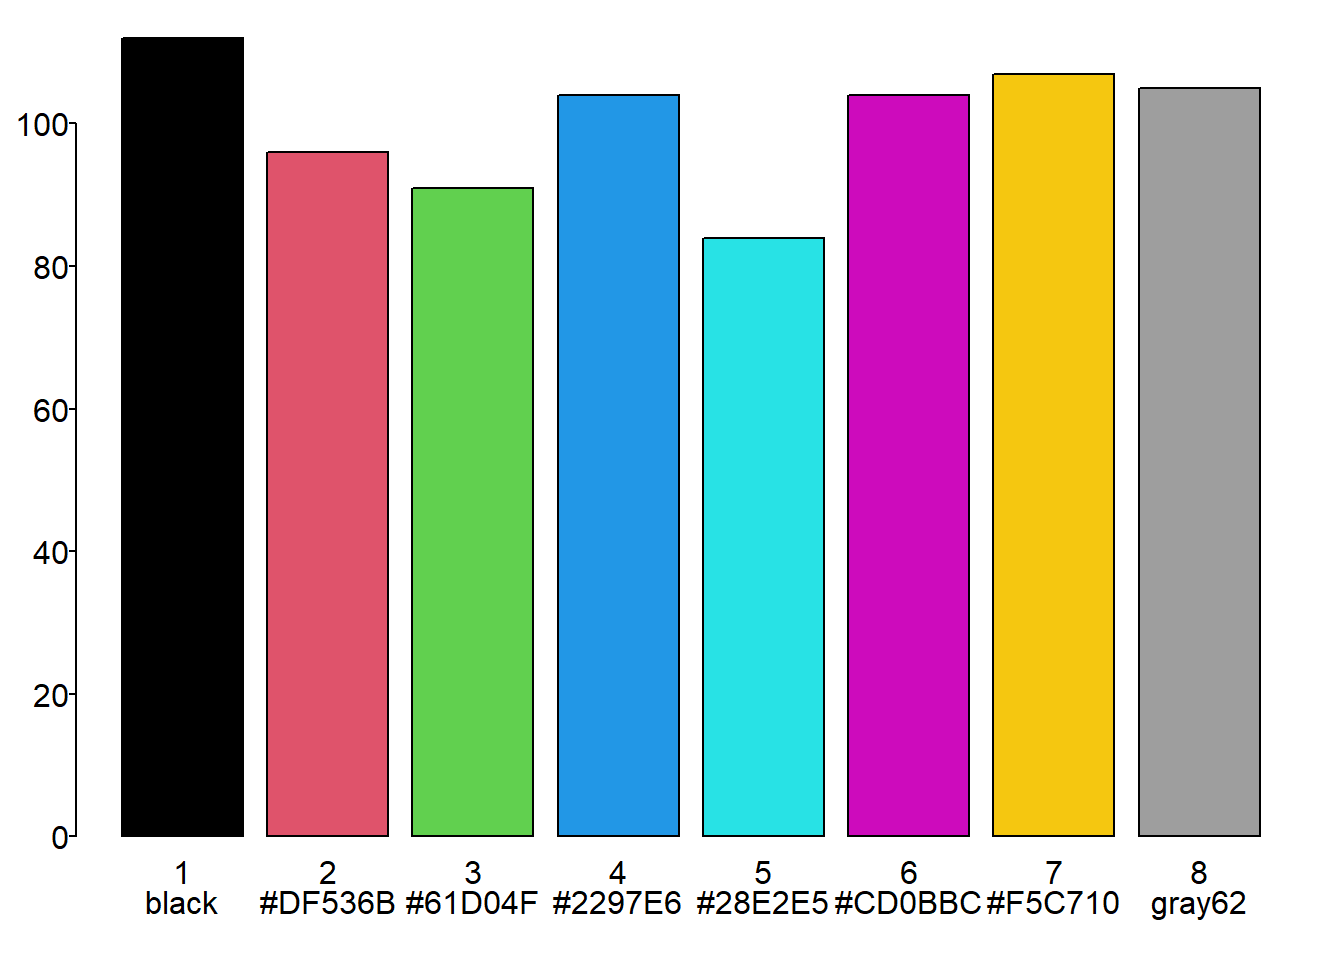
\includegraphics[width=0.9\linewidth]{41-Szinek_files/figure-latex/default-palette-1} 

}

\caption{Az alapértelmezett paletta 8 színének sorszáma és neve}\label{fig:default-palette}
\end{figure}

Más színeket is alapértelmezetté tehetünk, sőt a színek számát is megnövelhetjük a palettán. Ennek a legegyszerűbb módja, ha a \texttt{palette()} függvény argumentumában színkódokat tartalmazó karakteres vektort adunk meg.

\begin{Shaded}
\begin{Highlighting}[]
\NormalTok{szinek }\OtherTok{\textless{}{-}} \FunctionTok{c}\NormalTok{(}\StringTok{"\#E84F2C"}\NormalTok{, }\StringTok{"\#E31307"}\NormalTok{, }\StringTok{"\#E84F2C"}\NormalTok{, }\StringTok{"\#E4BA51"}\NormalTok{, }\StringTok{"\#E3B786"}\NormalTok{, }\StringTok{"\#825846"}\NormalTok{, }
    \StringTok{"\#59392A"}\NormalTok{, }\StringTok{"\#564C30"}\NormalTok{, }\StringTok{"\#897D6E"}\NormalTok{, }\StringTok{"\#627C82"}\NormalTok{, }\StringTok{"\#93AF8A"}\NormalTok{, }\StringTok{"\#A0BA5E"}\NormalTok{, }\StringTok{"\#63BA5E"}\NormalTok{, }
    \StringTok{"\#5EBAB2"}\NormalTok{, }\StringTok{"\#6596B7"}\NormalTok{)}
\FunctionTok{palette}\NormalTok{(}\AttributeTok{value =}\NormalTok{ szinek)}
\end{Highlighting}
\end{Shaded}

A rajzfüggvények ezután a paletta új színeit használják.

\begin{Shaded}
\begin{Highlighting}[]
\FunctionTok{barplot}\NormalTok{(x[}\DecValTok{1}\SpecialCharTok{:}\DecValTok{15}\NormalTok{], }\AttributeTok{col =} \DecValTok{1}\SpecialCharTok{:}\DecValTok{15}\NormalTok{)}
\end{Highlighting}
\end{Shaded}

\begin{center}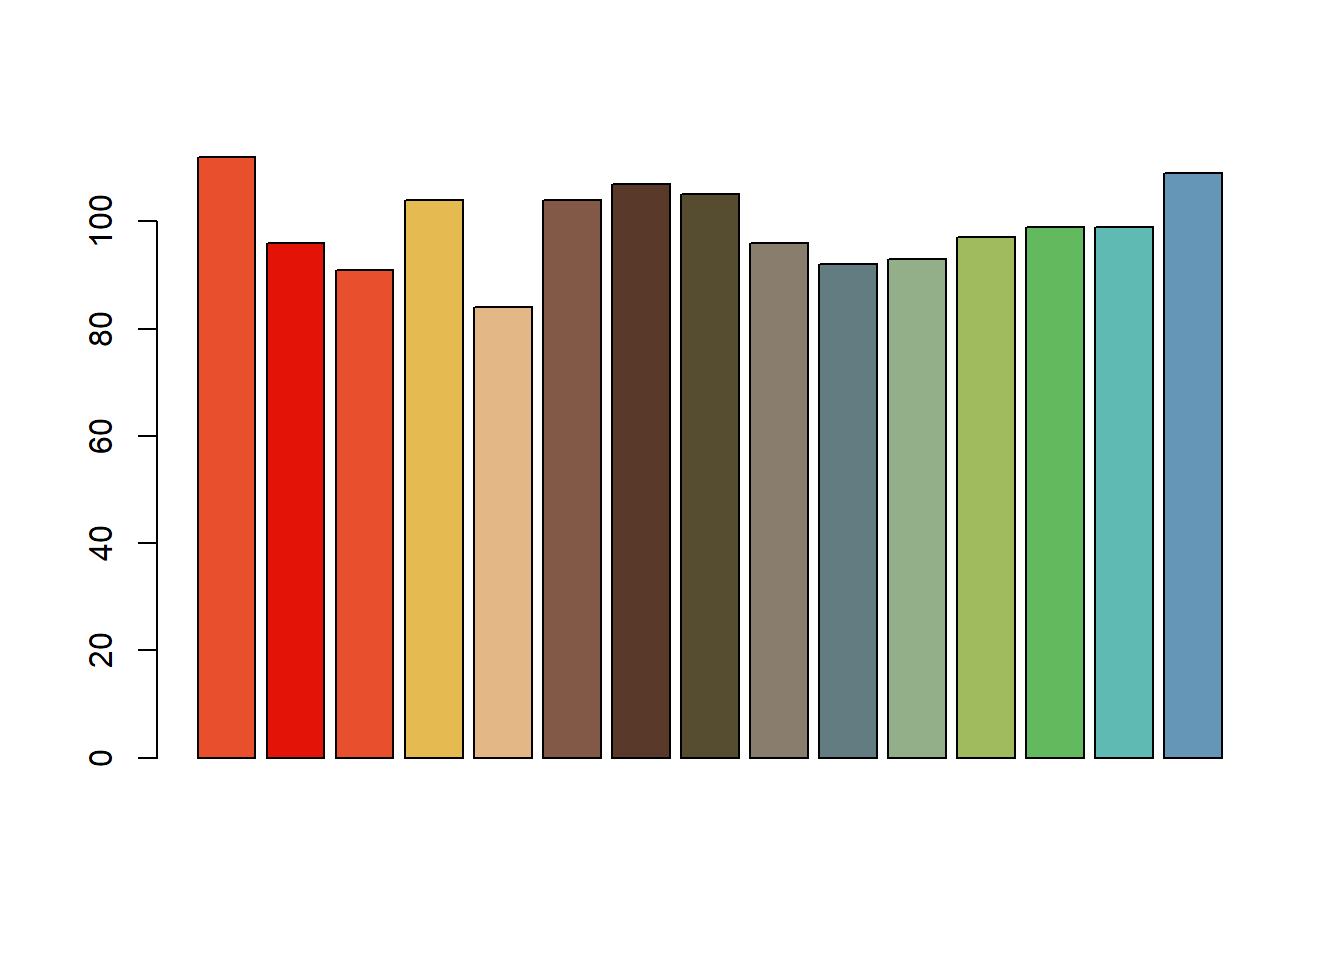
\includegraphics[width=0.9\linewidth]{41-Szinek_files/figure-latex/unnamed-chunk-2-1} \end{center}

Ha megváltoztattuk a paletta színeit, akkor az alapértelmezett színekhez a \texttt{palette("default")} paranccsal térhetünk vissza.

\begin{Shaded}
\begin{Highlighting}[]
\FunctionTok{palette}\NormalTok{(}\AttributeTok{value =} \StringTok{"default"}\NormalTok{)  }\CommentTok{\# alapértelmezett paletta visszaállítása}
\end{Highlighting}
\end{Shaded}

\hypertarget{szinek-valasztasa-rcolorbrewer}{%
\section{Színek választása az RColorBrewer csomag segítségével}\label{szinek-valasztasa-rcolorbrewer}}

Az \textbf{RColorBrewer} csomag \texttt{brewer.pal()} függvénye szolgál az előre definiált színpaletták alapján színkódokat tartalmazó vektor létrehozására. A függvény általános alakja:

\begin{Shaded}
\begin{Highlighting}[]
\FunctionTok{library}\NormalTok{(RColorBrewer)}
\FunctionTok{brewer.pal}\NormalTok{(n, name)}
\end{Highlighting}
\end{Shaded}

Az \texttt{n=} a kívánt színek számát határozza meg, amely háromnál nem lehet kevesebb. A \texttt{name=} a színpaletta nevét tartalmazza. A választható neveket a \texttt{brewer.pal.info} adattábla tartalmazza, amely a palettából elérhető összes szín számát és a paletta típusát is tartalmazza. Ez utóbbi a \texttt{category} oszlopban olvasható, amelynek lehetséges értékei: \texttt{seq}, \texttt{div} és \texttt{qual}. A szekvenciális palettákat (\texttt{seq}) rendezett adatok ábrázolására használhatjuk: a világosabb színek a kisebb értékeket, a sötétebbek a nagyobbakat szemléltethetik. A divergens (\texttt{div}) paletták a középső részt világosabb színekkel, a szélső értékeket sötétebb színekkel jelenítik meg. A kvalitatív (\texttt{qual}) paletta kategorikus változók megjelenítésére használható.

\begin{Shaded}
\begin{Highlighting}[]
\FunctionTok{library}\NormalTok{(RColorBrewer)}
\NormalTok{brewer.pal.info}
\CommentTok{\#\textgreater{}          maxcolors category colorblind}
\CommentTok{\#\textgreater{} BrBG            11      div       TRUE}
\CommentTok{\#\textgreater{} PiYG            11      div       TRUE}
\CommentTok{\#\textgreater{} PRGn            11      div       TRUE}
\CommentTok{\#\textgreater{} PuOr            11      div       TRUE}
\CommentTok{\#\textgreater{} RdBu            11      div       TRUE}
\CommentTok{\#\textgreater{} RdGy            11      div      FALSE}
\CommentTok{\#\textgreater{} RdYlBu          11      div       TRUE}
\CommentTok{\#\textgreater{} RdYlGn          11      div      FALSE}
\CommentTok{\#\textgreater{} Spectral        11      div      FALSE}
\CommentTok{\#\textgreater{} Accent           8     qual      FALSE}
\CommentTok{\#\textgreater{} Dark2            8     qual       TRUE}
\CommentTok{\#\textgreater{} Paired          12     qual       TRUE}
\CommentTok{\#\textgreater{} Pastel1          9     qual      FALSE}
\CommentTok{\#\textgreater{} Pastel2          8     qual      FALSE}
\CommentTok{\#\textgreater{} Set1             9     qual      FALSE}
\CommentTok{\#\textgreater{} Set2             8     qual       TRUE}
\CommentTok{\#\textgreater{} Set3            12     qual      FALSE}
\CommentTok{\#\textgreater{} Blues            9      seq       TRUE}
\CommentTok{\#\textgreater{} BuGn             9      seq       TRUE}
\CommentTok{\#\textgreater{} BuPu             9      seq       TRUE}
\CommentTok{\#\textgreater{} GnBu             9      seq       TRUE}
\CommentTok{\#\textgreater{} Greens           9      seq       TRUE}
\CommentTok{\#\textgreater{} Greys            9      seq       TRUE}
\CommentTok{\#\textgreater{} Oranges          9      seq       TRUE}
\CommentTok{\#\textgreater{} OrRd             9      seq       TRUE}
\CommentTok{\#\textgreater{} PuBu             9      seq       TRUE}
\CommentTok{\#\textgreater{} PuBuGn           9      seq       TRUE}
\CommentTok{\#\textgreater{} PuRd             9      seq       TRUE}
\CommentTok{\#\textgreater{} Purples          9      seq       TRUE}
\CommentTok{\#\textgreater{} RdPu             9      seq       TRUE}
\CommentTok{\#\textgreater{} Reds             9      seq       TRUE}
\CommentTok{\#\textgreater{} YlGn             9      seq       TRUE}
\CommentTok{\#\textgreater{} YlGnBu           9      seq       TRUE}
\CommentTok{\#\textgreater{} YlOrBr           9      seq       TRUE}
\CommentTok{\#\textgreater{} YlOrRd           9      seq       TRUE}
\end{Highlighting}
\end{Shaded}

A továbbiakban a \texttt{brewer.pal()} függvény használatára mutatunk példát:

\begin{Shaded}
\begin{Highlighting}[]
\CommentTok{\# az x adatvektor beállítása}
\FunctionTok{set.seed}\NormalTok{(}\DecValTok{0}\NormalTok{)}
\NormalTok{x }\OtherTok{\textless{}{-}} \FunctionTok{rpois}\NormalTok{(}\AttributeTok{n =} \DecValTok{50}\NormalTok{, }\AttributeTok{lambda =} \DecValTok{100}\NormalTok{)}
\CommentTok{\# grafikus paraméterek beállítása}
\FunctionTok{par}\NormalTok{(}\AttributeTok{las =} \DecValTok{1}\NormalTok{, }\AttributeTok{mgp =} \FunctionTok{c}\NormalTok{(}\DecValTok{0}\NormalTok{, }\FloatTok{0.2}\NormalTok{, }\DecValTok{0}\NormalTok{), }\AttributeTok{tcl =} \SpecialCharTok{{-}}\FloatTok{0.2}\NormalTok{, }\AttributeTok{mar =} \FunctionTok{c}\NormalTok{(}\DecValTok{3}\NormalTok{, }\DecValTok{2}\NormalTok{, }\DecValTok{1}\NormalTok{, }\DecValTok{1}\NormalTok{))}
\FunctionTok{library}\NormalTok{(RColorBrewer)}
\FunctionTok{par}\NormalTok{(}\AttributeTok{mfrow =} \FunctionTok{c}\NormalTok{(}\DecValTok{1}\NormalTok{, }\DecValTok{2}\NormalTok{))}
\FunctionTok{barplot}\NormalTok{(x[}\DecValTok{1}\SpecialCharTok{:}\DecValTok{11}\NormalTok{], }\AttributeTok{col =} \FunctionTok{brewer.pal}\NormalTok{(}\AttributeTok{n =} \DecValTok{11}\NormalTok{, }\AttributeTok{name =} \StringTok{"BrBG"}\NormalTok{), }\AttributeTok{names.arg =} \DecValTok{1}\SpecialCharTok{:}\DecValTok{11}\NormalTok{, }
    \AttributeTok{main =} \StringTok{"BrBG, div"}\NormalTok{)}
\FunctionTok{barplot}\NormalTok{(x[}\DecValTok{1}\SpecialCharTok{:}\DecValTok{11}\NormalTok{], }\AttributeTok{col =} \FunctionTok{brewer.pal}\NormalTok{(}\AttributeTok{n =} \DecValTok{11}\NormalTok{, }\AttributeTok{name =} \StringTok{"BrBG"}\NormalTok{), }\AttributeTok{names.arg =} \DecValTok{1}\SpecialCharTok{:}\DecValTok{11}\NormalTok{, }
    \AttributeTok{main =} \StringTok{"BrBG, div"}\NormalTok{, }\AttributeTok{border =} \ConstantTok{NA}\NormalTok{)}
\end{Highlighting}
\end{Shaded}

\begin{center}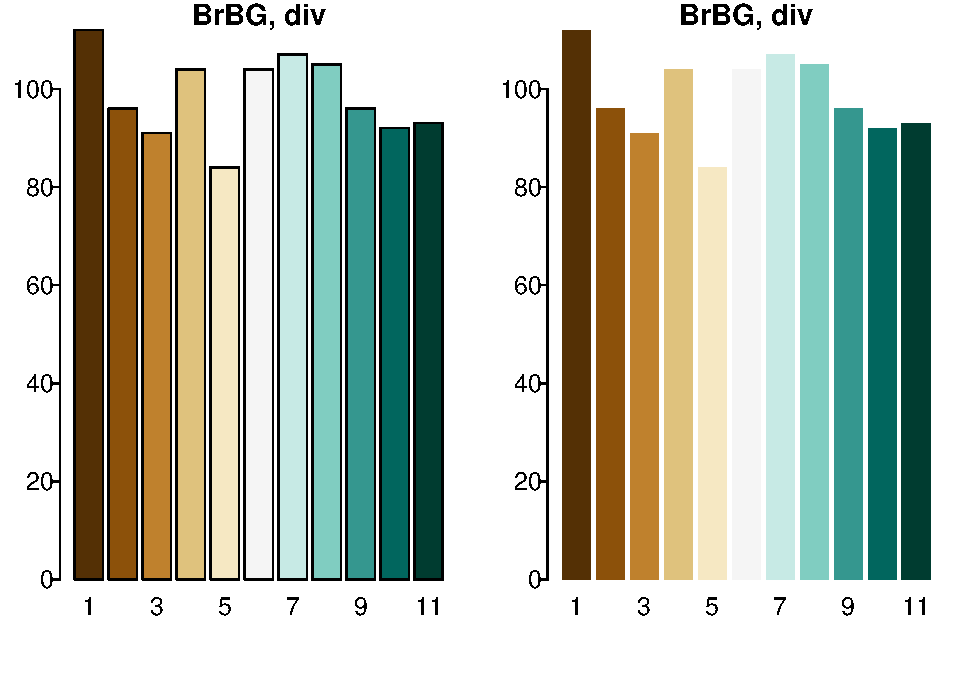
\includegraphics[width=0.9\linewidth]{41-Szinek_files/figure-latex/unnamed-chunk-6-1} \end{center}

\begin{Shaded}
\begin{Highlighting}[]
\FunctionTok{par}\NormalTok{(}\AttributeTok{mfrow =} \FunctionTok{c}\NormalTok{(}\DecValTok{1}\NormalTok{, }\DecValTok{2}\NormalTok{))}
\FunctionTok{barplot}\NormalTok{(x[}\DecValTok{1}\SpecialCharTok{:}\DecValTok{11}\NormalTok{], }\AttributeTok{col =} \FunctionTok{brewer.pal}\NormalTok{(}\AttributeTok{n =} \DecValTok{11}\NormalTok{, }\AttributeTok{name =} \StringTok{"PiYG"}\NormalTok{), }\AttributeTok{names.arg =} \DecValTok{1}\SpecialCharTok{:}\DecValTok{11}\NormalTok{, }
    \AttributeTok{main =} \StringTok{"PiYG, div"}\NormalTok{)}
\FunctionTok{barplot}\NormalTok{(x[}\DecValTok{1}\SpecialCharTok{:}\DecValTok{11}\NormalTok{], }\AttributeTok{col =} \FunctionTok{brewer.pal}\NormalTok{(}\AttributeTok{n =} \DecValTok{11}\NormalTok{, }\AttributeTok{name =} \StringTok{"PiYG"}\NormalTok{), }\AttributeTok{names.arg =} \DecValTok{1}\SpecialCharTok{:}\DecValTok{11}\NormalTok{, }
    \AttributeTok{main =} \StringTok{"PiYG, div"}\NormalTok{, }\AttributeTok{border =} \ConstantTok{NA}\NormalTok{)}
\end{Highlighting}
\end{Shaded}

\begin{center}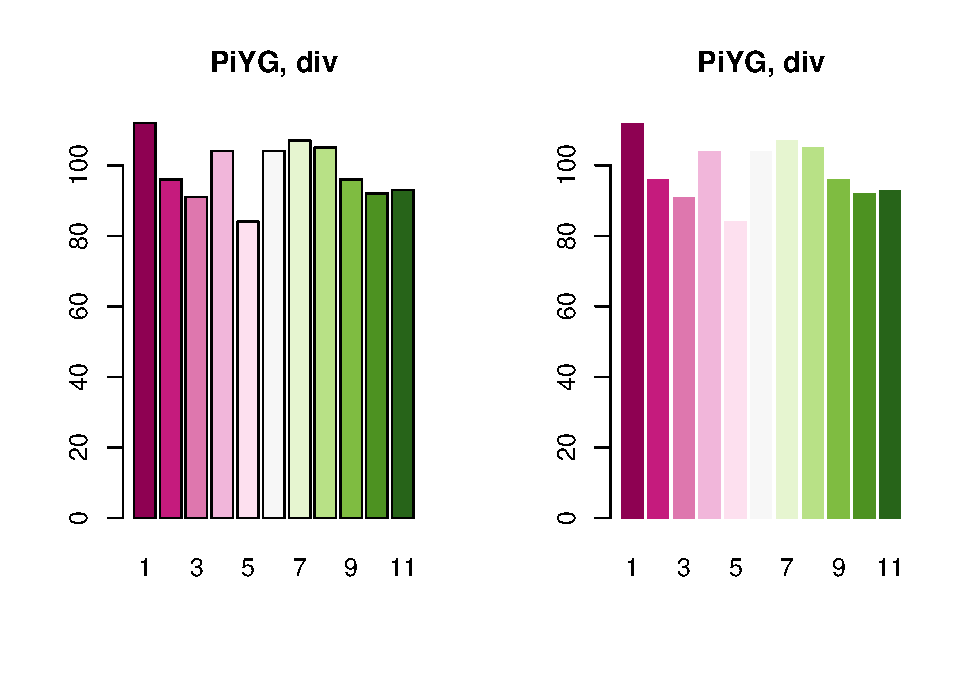
\includegraphics[width=0.9\linewidth]{41-Szinek_files/figure-latex/unnamed-chunk-7-1} \end{center}

\begin{Shaded}
\begin{Highlighting}[]
\FunctionTok{par}\NormalTok{(}\AttributeTok{mfrow =} \FunctionTok{c}\NormalTok{(}\DecValTok{1}\NormalTok{, }\DecValTok{2}\NormalTok{))}
\FunctionTok{barplot}\NormalTok{(x[}\DecValTok{1}\SpecialCharTok{:}\DecValTok{11}\NormalTok{], }\AttributeTok{col =} \FunctionTok{brewer.pal}\NormalTok{(}\AttributeTok{n =} \DecValTok{11}\NormalTok{, }\AttributeTok{name =} \StringTok{"PRGn"}\NormalTok{), }\AttributeTok{names.arg =} \DecValTok{1}\SpecialCharTok{:}\DecValTok{11}\NormalTok{, }
    \AttributeTok{main =} \StringTok{"PRGn, div"}\NormalTok{)}
\FunctionTok{barplot}\NormalTok{(x[}\DecValTok{1}\SpecialCharTok{:}\DecValTok{11}\NormalTok{], }\AttributeTok{col =} \FunctionTok{brewer.pal}\NormalTok{(}\AttributeTok{n =} \DecValTok{11}\NormalTok{, }\AttributeTok{name =} \StringTok{"PRGn"}\NormalTok{), }\AttributeTok{names.arg =} \DecValTok{1}\SpecialCharTok{:}\DecValTok{11}\NormalTok{, }
    \AttributeTok{main =} \StringTok{"PRGn, div"}\NormalTok{, }\AttributeTok{border =} \ConstantTok{NA}\NormalTok{)}
\end{Highlighting}
\end{Shaded}

\begin{center}\includegraphics[width=0.9\linewidth]{41-Szinek_files/figure-latex/unnamed-chunk-8-1} \end{center}

\begin{Shaded}
\begin{Highlighting}[]
\FunctionTok{par}\NormalTok{(}\AttributeTok{mfrow =} \FunctionTok{c}\NormalTok{(}\DecValTok{1}\NormalTok{, }\DecValTok{2}\NormalTok{))}
\FunctionTok{barplot}\NormalTok{(x[}\DecValTok{1}\SpecialCharTok{:}\DecValTok{11}\NormalTok{], }\AttributeTok{col =} \FunctionTok{brewer.pal}\NormalTok{(}\AttributeTok{n =} \DecValTok{11}\NormalTok{, }\AttributeTok{name =} \StringTok{"PuOr"}\NormalTok{), }\AttributeTok{names.arg =} \DecValTok{1}\SpecialCharTok{:}\DecValTok{11}\NormalTok{, }
    \AttributeTok{main =} \StringTok{"PuOr, div"}\NormalTok{)}
\FunctionTok{barplot}\NormalTok{(x[}\DecValTok{1}\SpecialCharTok{:}\DecValTok{11}\NormalTok{], }\AttributeTok{col =} \FunctionTok{brewer.pal}\NormalTok{(}\AttributeTok{n =} \DecValTok{11}\NormalTok{, }\AttributeTok{name =} \StringTok{"PuOr"}\NormalTok{), }\AttributeTok{names.arg =} \DecValTok{1}\SpecialCharTok{:}\DecValTok{11}\NormalTok{, }
    \AttributeTok{main =} \StringTok{"PuOr, div"}\NormalTok{, }\AttributeTok{border =} \ConstantTok{NA}\NormalTok{)}
\end{Highlighting}
\end{Shaded}

\begin{center}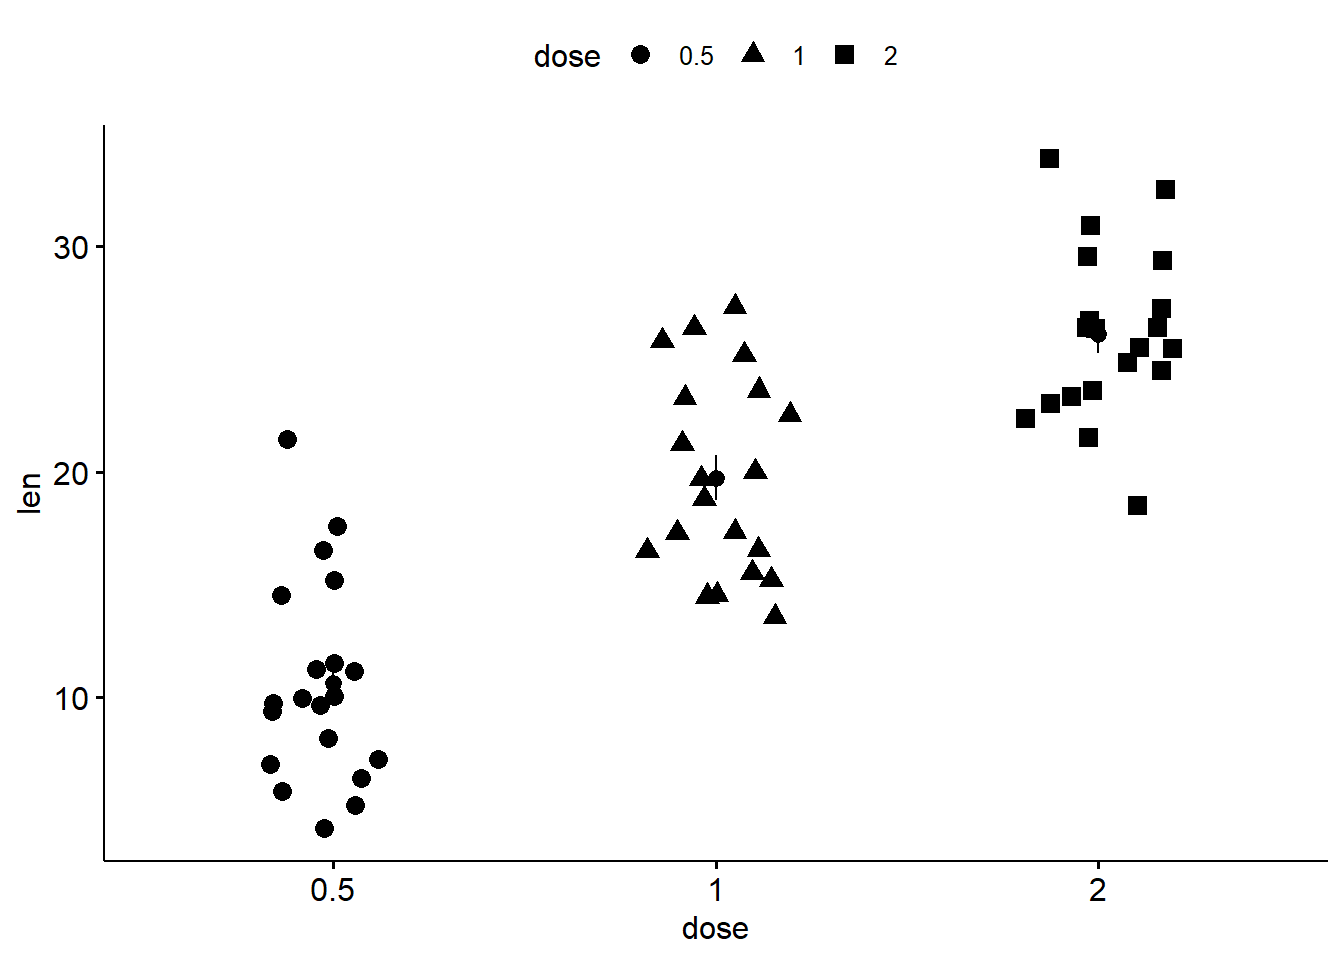
\includegraphics[width=0.9\linewidth]{41-Szinek_files/figure-latex/unnamed-chunk-9-1} \end{center}

\begin{Shaded}
\begin{Highlighting}[]
\FunctionTok{par}\NormalTok{(}\AttributeTok{mfrow =} \FunctionTok{c}\NormalTok{(}\DecValTok{1}\NormalTok{, }\DecValTok{2}\NormalTok{))}
\FunctionTok{barplot}\NormalTok{(x[}\DecValTok{1}\SpecialCharTok{:}\DecValTok{11}\NormalTok{], }\AttributeTok{col =} \FunctionTok{brewer.pal}\NormalTok{(}\AttributeTok{n =} \DecValTok{11}\NormalTok{, }\AttributeTok{name =} \StringTok{"RdBu"}\NormalTok{), }\AttributeTok{names.arg =} \DecValTok{1}\SpecialCharTok{:}\DecValTok{11}\NormalTok{, }
    \AttributeTok{main =} \StringTok{"RdBu, div"}\NormalTok{)}
\FunctionTok{barplot}\NormalTok{(x[}\DecValTok{1}\SpecialCharTok{:}\DecValTok{11}\NormalTok{], }\AttributeTok{col =} \FunctionTok{brewer.pal}\NormalTok{(}\AttributeTok{n =} \DecValTok{11}\NormalTok{, }\AttributeTok{name =} \StringTok{"RdBu"}\NormalTok{), }\AttributeTok{names.arg =} \DecValTok{1}\SpecialCharTok{:}\DecValTok{11}\NormalTok{, }
    \AttributeTok{main =} \StringTok{"RdBu, div"}\NormalTok{, }\AttributeTok{border =} \ConstantTok{NA}\NormalTok{)}
\end{Highlighting}
\end{Shaded}

\begin{center}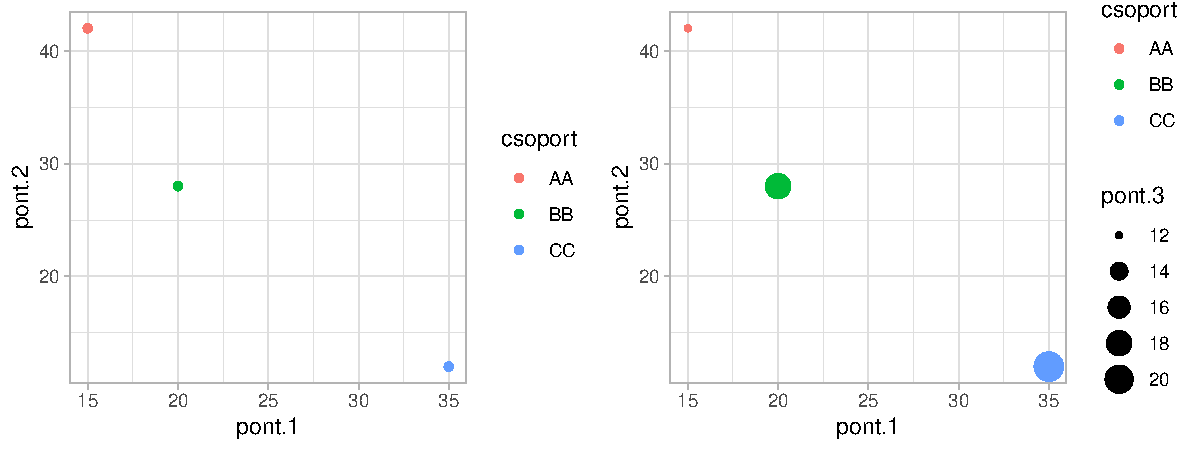
\includegraphics[width=0.9\linewidth]{41-Szinek_files/figure-latex/unnamed-chunk-10-1} \end{center}

\begin{Shaded}
\begin{Highlighting}[]
\FunctionTok{par}\NormalTok{(}\AttributeTok{mfrow =} \FunctionTok{c}\NormalTok{(}\DecValTok{1}\NormalTok{, }\DecValTok{2}\NormalTok{))}
\FunctionTok{barplot}\NormalTok{(x[}\DecValTok{1}\SpecialCharTok{:}\DecValTok{11}\NormalTok{], }\AttributeTok{col =} \FunctionTok{brewer.pal}\NormalTok{(}\AttributeTok{n =} \DecValTok{11}\NormalTok{, }\AttributeTok{name =} \StringTok{"RdGy"}\NormalTok{), }\AttributeTok{names.arg =} \DecValTok{1}\SpecialCharTok{:}\DecValTok{11}\NormalTok{, }
    \AttributeTok{main =} \StringTok{"RdGy, div"}\NormalTok{)}
\FunctionTok{barplot}\NormalTok{(x[}\DecValTok{1}\SpecialCharTok{:}\DecValTok{11}\NormalTok{], }\AttributeTok{col =} \FunctionTok{brewer.pal}\NormalTok{(}\AttributeTok{n =} \DecValTok{11}\NormalTok{, }\AttributeTok{name =} \StringTok{"RdGy"}\NormalTok{), }\AttributeTok{names.arg =} \DecValTok{1}\SpecialCharTok{:}\DecValTok{11}\NormalTok{, }
    \AttributeTok{main =} \StringTok{"RdGy, div"}\NormalTok{, }\AttributeTok{border =} \ConstantTok{NA}\NormalTok{)}
\end{Highlighting}
\end{Shaded}

\begin{center}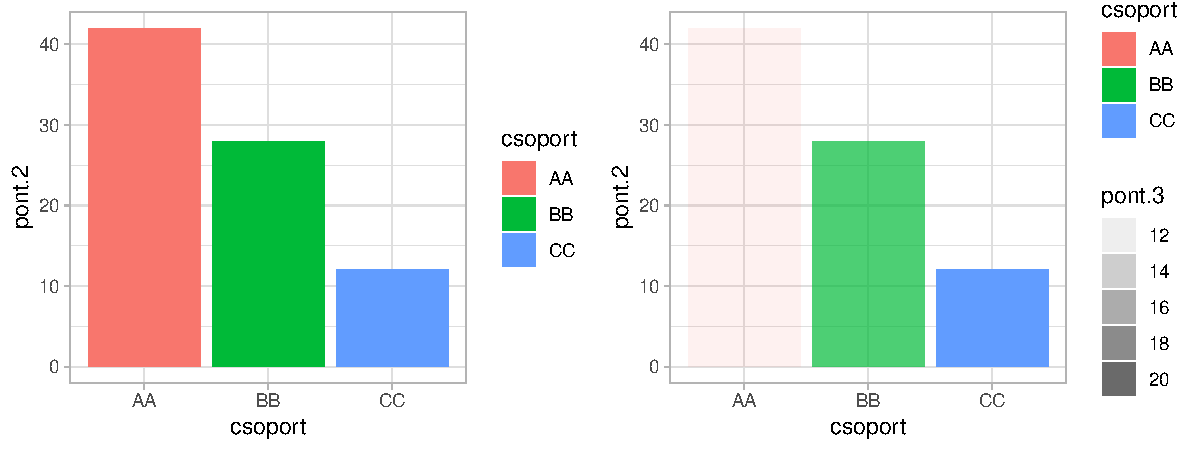
\includegraphics[width=0.9\linewidth]{41-Szinek_files/figure-latex/unnamed-chunk-11-1} \end{center}

\begin{Shaded}
\begin{Highlighting}[]
\FunctionTok{par}\NormalTok{(}\AttributeTok{mfrow =} \FunctionTok{c}\NormalTok{(}\DecValTok{1}\NormalTok{, }\DecValTok{2}\NormalTok{))}
\FunctionTok{barplot}\NormalTok{(x[}\DecValTok{1}\SpecialCharTok{:}\DecValTok{11}\NormalTok{], }\AttributeTok{col =} \FunctionTok{brewer.pal}\NormalTok{(}\AttributeTok{n =} \DecValTok{11}\NormalTok{, }\AttributeTok{name =} \StringTok{"RdYlBu"}\NormalTok{), }\AttributeTok{names.arg =} \DecValTok{1}\SpecialCharTok{:}\DecValTok{11}\NormalTok{, }
    \AttributeTok{main =} \StringTok{"RdYlBu, div"}\NormalTok{)}
\FunctionTok{barplot}\NormalTok{(x[}\DecValTok{1}\SpecialCharTok{:}\DecValTok{11}\NormalTok{], }\AttributeTok{col =} \FunctionTok{brewer.pal}\NormalTok{(}\AttributeTok{n =} \DecValTok{11}\NormalTok{, }\AttributeTok{name =} \StringTok{"RdYlBu"}\NormalTok{), }\AttributeTok{names.arg =} \DecValTok{1}\SpecialCharTok{:}\DecValTok{11}\NormalTok{, }
    \AttributeTok{main =} \StringTok{"RdYlBu, div"}\NormalTok{, }\AttributeTok{border =} \ConstantTok{NA}\NormalTok{)}
\end{Highlighting}
\end{Shaded}

\begin{center}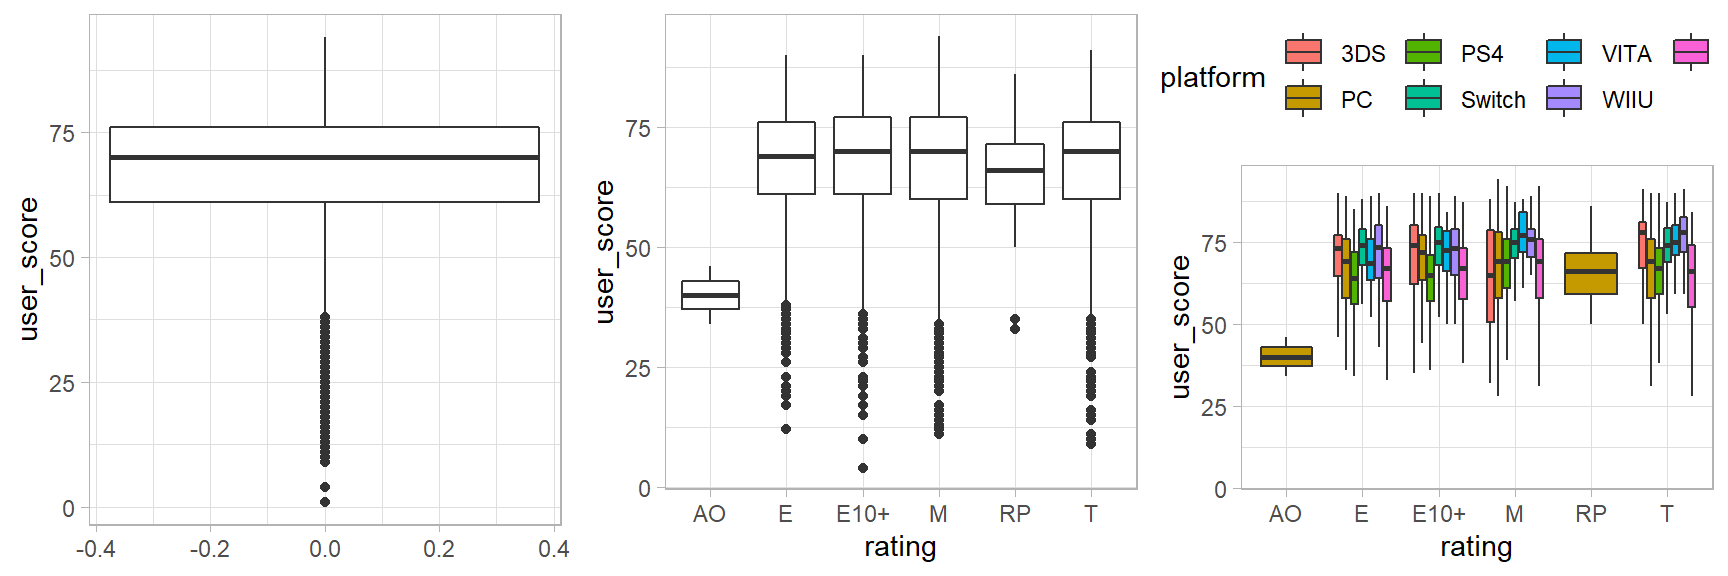
\includegraphics[width=0.9\linewidth]{41-Szinek_files/figure-latex/unnamed-chunk-12-1} \end{center}

\begin{Shaded}
\begin{Highlighting}[]
\FunctionTok{par}\NormalTok{(}\AttributeTok{mfrow =} \FunctionTok{c}\NormalTok{(}\DecValTok{1}\NormalTok{, }\DecValTok{2}\NormalTok{))}
\FunctionTok{barplot}\NormalTok{(x[}\DecValTok{1}\SpecialCharTok{:}\DecValTok{11}\NormalTok{], }\AttributeTok{col =} \FunctionTok{brewer.pal}\NormalTok{(}\AttributeTok{n =} \DecValTok{11}\NormalTok{, }\AttributeTok{name =} \StringTok{"RdYlGn"}\NormalTok{), }\AttributeTok{names.arg =} \DecValTok{1}\SpecialCharTok{:}\DecValTok{11}\NormalTok{, }
    \AttributeTok{main =} \StringTok{"RdYlGn, div"}\NormalTok{)}
\FunctionTok{barplot}\NormalTok{(x[}\DecValTok{1}\SpecialCharTok{:}\DecValTok{11}\NormalTok{], }\AttributeTok{col =} \FunctionTok{brewer.pal}\NormalTok{(}\AttributeTok{n =} \DecValTok{11}\NormalTok{, }\AttributeTok{name =} \StringTok{"RdYlGn"}\NormalTok{), }\AttributeTok{names.arg =} \DecValTok{1}\SpecialCharTok{:}\DecValTok{11}\NormalTok{, }
    \AttributeTok{main =} \StringTok{"RdYlGn, div"}\NormalTok{, }\AttributeTok{border =} \ConstantTok{NA}\NormalTok{)}
\end{Highlighting}
\end{Shaded}

\begin{center}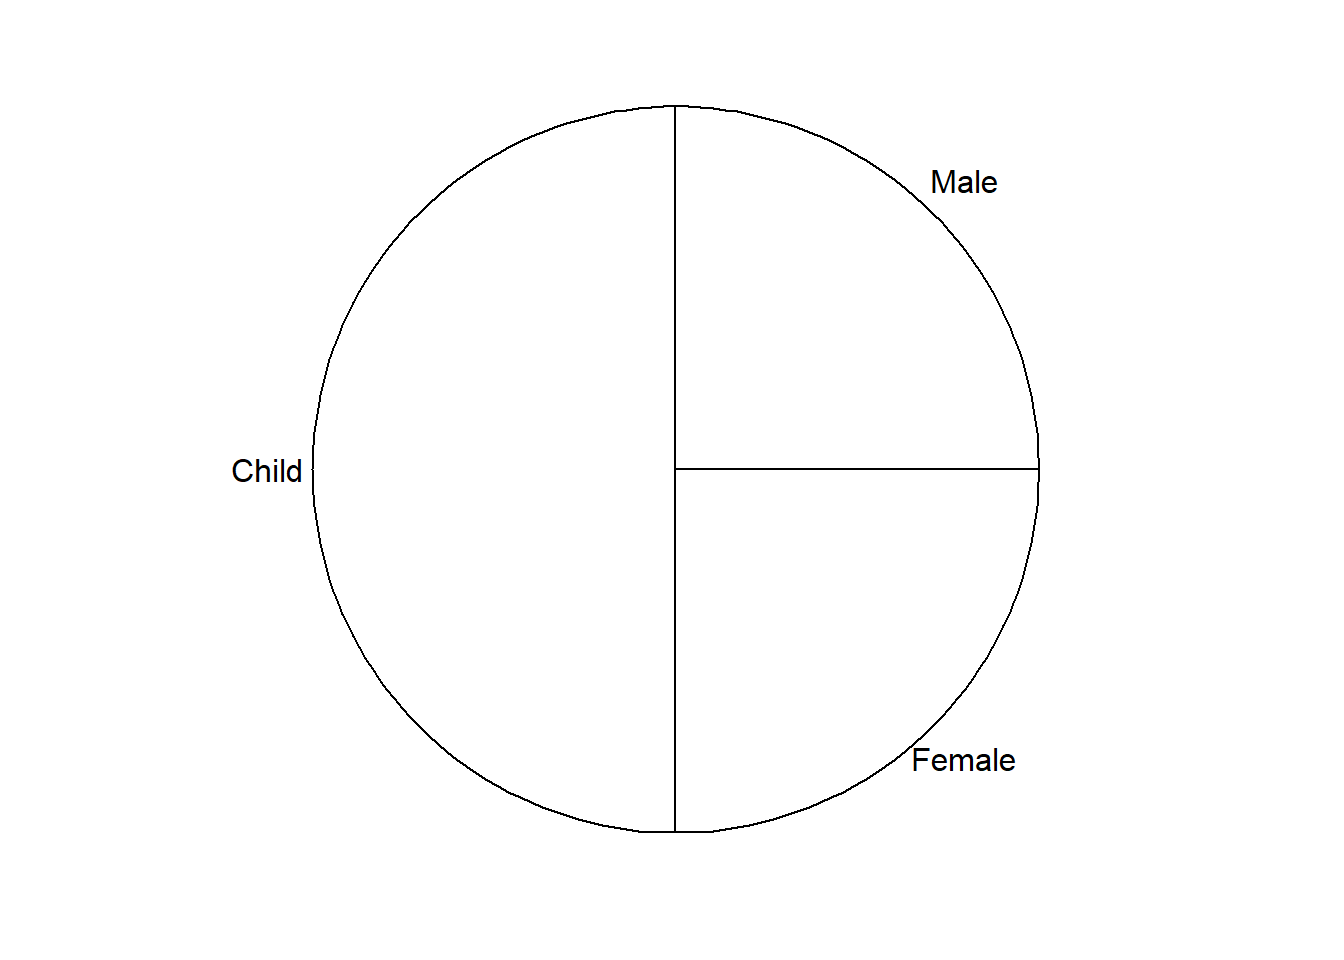
\includegraphics[width=0.9\linewidth]{41-Szinek_files/figure-latex/unnamed-chunk-13-1} \end{center}

\begin{Shaded}
\begin{Highlighting}[]
\FunctionTok{par}\NormalTok{(}\AttributeTok{mfrow =} \FunctionTok{c}\NormalTok{(}\DecValTok{1}\NormalTok{, }\DecValTok{2}\NormalTok{))}
\FunctionTok{barplot}\NormalTok{(x[}\DecValTok{1}\SpecialCharTok{:}\DecValTok{11}\NormalTok{], }\AttributeTok{col =} \FunctionTok{brewer.pal}\NormalTok{(}\AttributeTok{n =} \DecValTok{11}\NormalTok{, }\AttributeTok{name =} \StringTok{"Spectral"}\NormalTok{), }\AttributeTok{names.arg =} \DecValTok{1}\SpecialCharTok{:}\DecValTok{11}\NormalTok{, }
    \AttributeTok{main =} \StringTok{"Spectral, div"}\NormalTok{)}
\FunctionTok{barplot}\NormalTok{(x[}\DecValTok{1}\SpecialCharTok{:}\DecValTok{11}\NormalTok{], }\AttributeTok{col =} \FunctionTok{brewer.pal}\NormalTok{(}\AttributeTok{n =} \DecValTok{11}\NormalTok{, }\AttributeTok{name =} \StringTok{"Spectral"}\NormalTok{), }\AttributeTok{names.arg =} \DecValTok{1}\SpecialCharTok{:}\DecValTok{11}\NormalTok{, }
    \AttributeTok{main =} \StringTok{"Spectral, div"}\NormalTok{, }\AttributeTok{border =} \ConstantTok{NA}\NormalTok{)}
\end{Highlighting}
\end{Shaded}

\begin{center}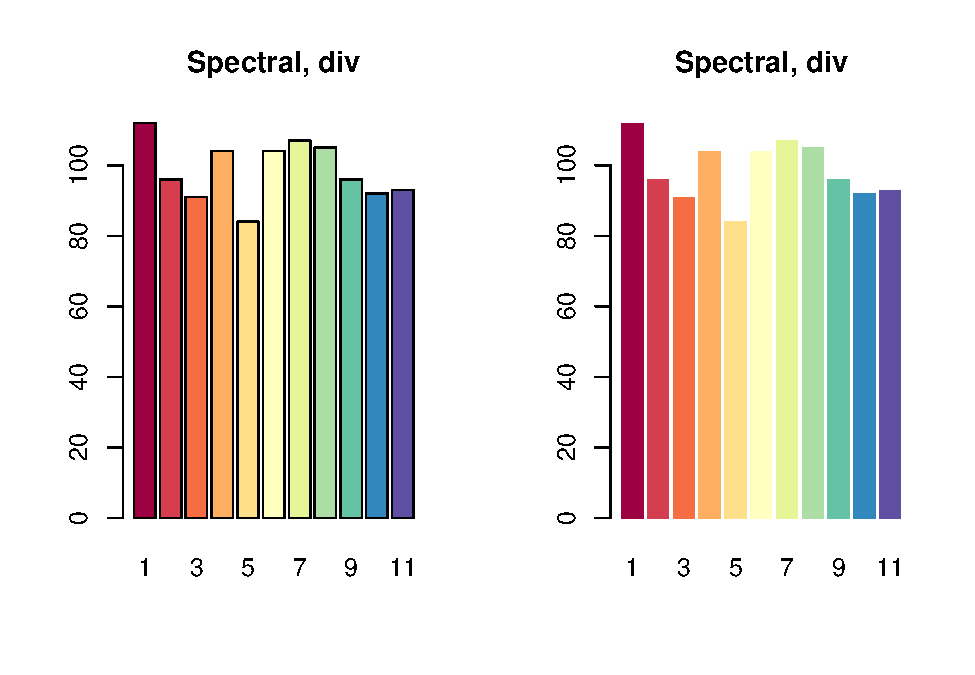
\includegraphics[width=0.9\linewidth]{41-Szinek_files/figure-latex/unnamed-chunk-14-1} \end{center}

\begin{Shaded}
\begin{Highlighting}[]
\FunctionTok{par}\NormalTok{(}\AttributeTok{mfrow =} \FunctionTok{c}\NormalTok{(}\DecValTok{1}\NormalTok{, }\DecValTok{2}\NormalTok{))}
\FunctionTok{barplot}\NormalTok{(x[}\DecValTok{1}\SpecialCharTok{:}\DecValTok{8}\NormalTok{], }\AttributeTok{col =} \FunctionTok{brewer.pal}\NormalTok{(}\AttributeTok{n =} \DecValTok{8}\NormalTok{, }\AttributeTok{name =} \StringTok{"Accent"}\NormalTok{), }\AttributeTok{names.arg =} \DecValTok{1}\SpecialCharTok{:}\DecValTok{8}\NormalTok{, }\AttributeTok{main =} \StringTok{"Accent, qual"}\NormalTok{)}
\FunctionTok{barplot}\NormalTok{(x[}\DecValTok{1}\SpecialCharTok{:}\DecValTok{8}\NormalTok{], }\AttributeTok{col =} \FunctionTok{brewer.pal}\NormalTok{(}\AttributeTok{n =} \DecValTok{8}\NormalTok{, }\AttributeTok{name =} \StringTok{"Accent"}\NormalTok{), }\AttributeTok{names.arg =} \DecValTok{1}\SpecialCharTok{:}\DecValTok{8}\NormalTok{, }\AttributeTok{main =} \StringTok{"Accent, qual"}\NormalTok{, }
    \AttributeTok{border =} \ConstantTok{NA}\NormalTok{)}
\end{Highlighting}
\end{Shaded}

\begin{center}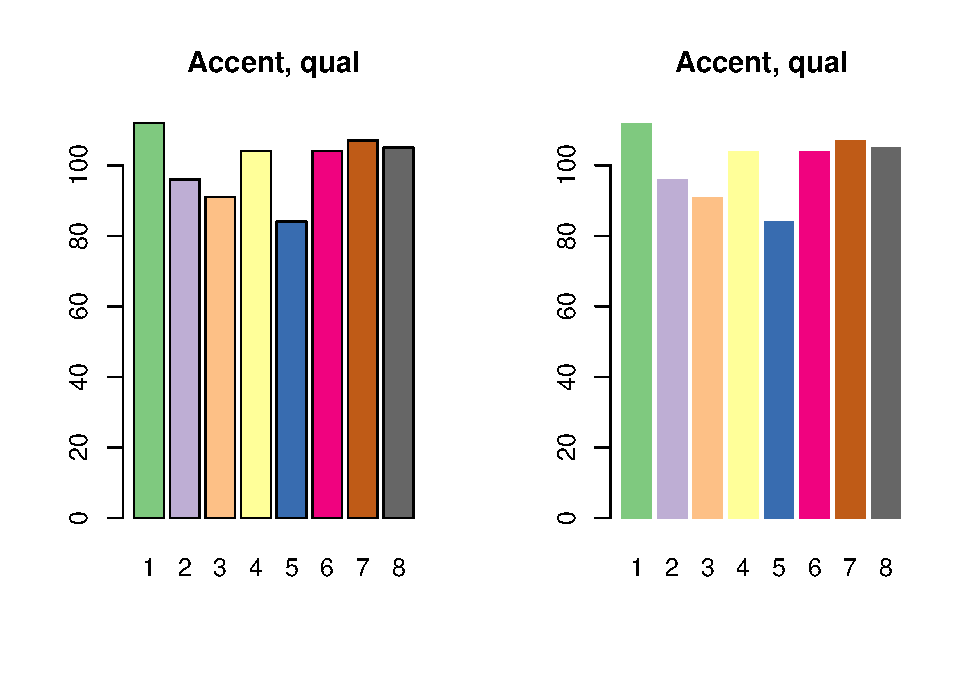
\includegraphics[width=0.9\linewidth]{41-Szinek_files/figure-latex/unnamed-chunk-15-1} \end{center}

\begin{Shaded}
\begin{Highlighting}[]
\FunctionTok{par}\NormalTok{(}\AttributeTok{mfrow =} \FunctionTok{c}\NormalTok{(}\DecValTok{1}\NormalTok{, }\DecValTok{2}\NormalTok{))}
\FunctionTok{barplot}\NormalTok{(x[}\DecValTok{1}\SpecialCharTok{:}\DecValTok{8}\NormalTok{], }\AttributeTok{col =} \FunctionTok{brewer.pal}\NormalTok{(}\AttributeTok{n =} \DecValTok{8}\NormalTok{, }\AttributeTok{name =} \StringTok{"Dark2"}\NormalTok{), }\AttributeTok{names.arg =} \DecValTok{1}\SpecialCharTok{:}\DecValTok{8}\NormalTok{, }\AttributeTok{main =} \StringTok{"Dark2, qual"}\NormalTok{)}
\FunctionTok{barplot}\NormalTok{(x[}\DecValTok{1}\SpecialCharTok{:}\DecValTok{8}\NormalTok{], }\AttributeTok{col =} \FunctionTok{brewer.pal}\NormalTok{(}\AttributeTok{n =} \DecValTok{8}\NormalTok{, }\AttributeTok{name =} \StringTok{"Dark2"}\NormalTok{), }\AttributeTok{names.arg =} \DecValTok{1}\SpecialCharTok{:}\DecValTok{8}\NormalTok{, }\AttributeTok{main =} \StringTok{"Dark2, qual"}\NormalTok{, }
    \AttributeTok{border =} \ConstantTok{NA}\NormalTok{)}
\end{Highlighting}
\end{Shaded}

\begin{center}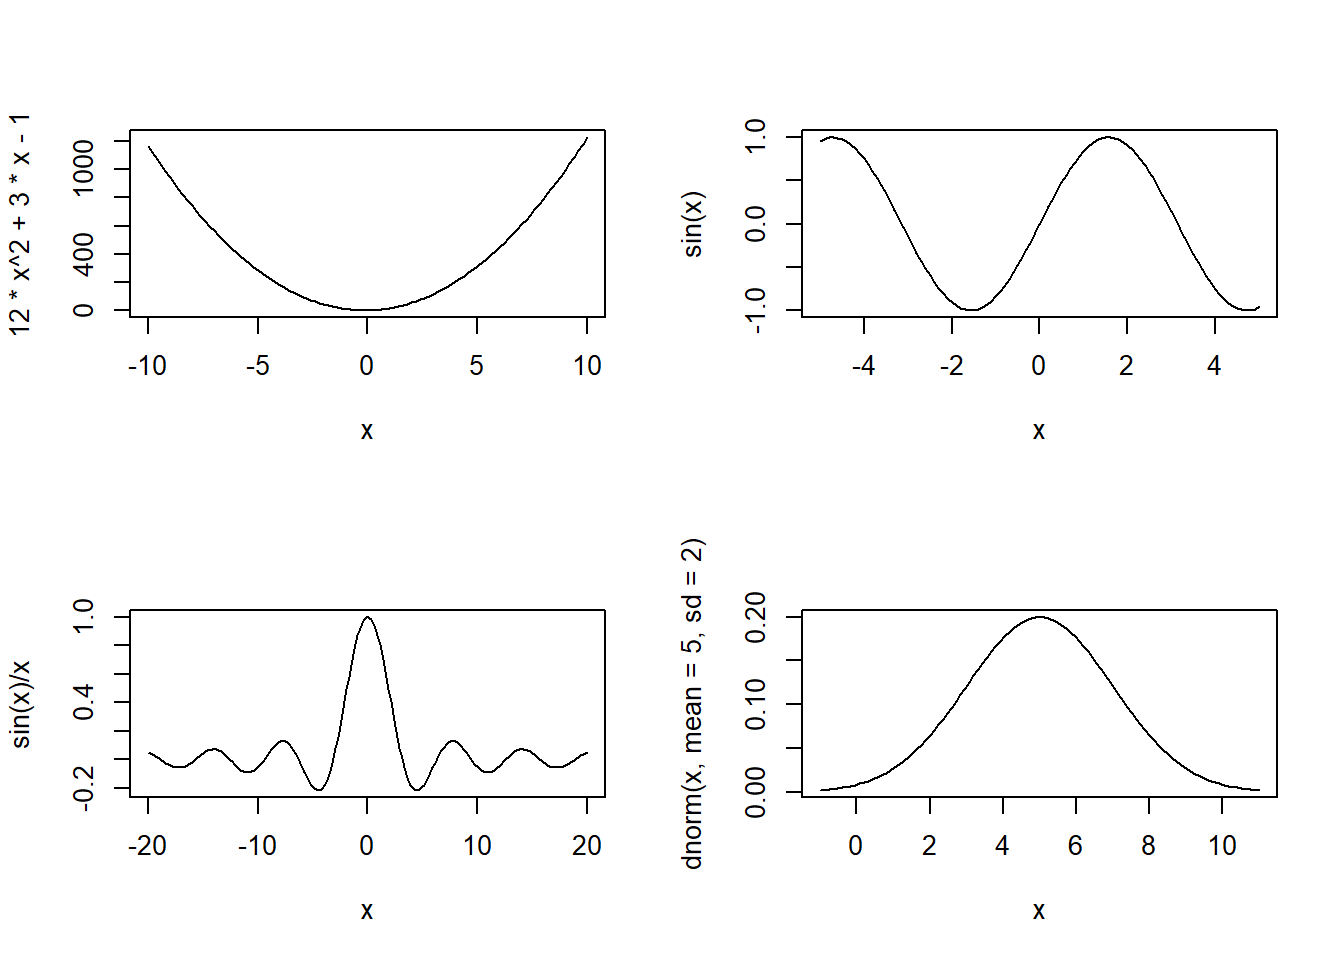
\includegraphics[width=0.9\linewidth]{41-Szinek_files/figure-latex/unnamed-chunk-16-1} \end{center}

\begin{Shaded}
\begin{Highlighting}[]
\FunctionTok{par}\NormalTok{(}\AttributeTok{mfrow =} \FunctionTok{c}\NormalTok{(}\DecValTok{1}\NormalTok{, }\DecValTok{2}\NormalTok{))}
\FunctionTok{barplot}\NormalTok{(x[}\DecValTok{1}\SpecialCharTok{:}\DecValTok{12}\NormalTok{], }\AttributeTok{col =} \FunctionTok{brewer.pal}\NormalTok{(}\AttributeTok{n =} \DecValTok{12}\NormalTok{, }\AttributeTok{name =} \StringTok{"Paired"}\NormalTok{), }\AttributeTok{names.arg =} \DecValTok{1}\SpecialCharTok{:}\DecValTok{12}\NormalTok{, }
    \AttributeTok{main =} \StringTok{"Paired, qual"}\NormalTok{)}
\FunctionTok{barplot}\NormalTok{(x[}\DecValTok{1}\SpecialCharTok{:}\DecValTok{12}\NormalTok{], }\AttributeTok{col =} \FunctionTok{brewer.pal}\NormalTok{(}\AttributeTok{n =} \DecValTok{12}\NormalTok{, }\AttributeTok{name =} \StringTok{"Paired"}\NormalTok{), }\AttributeTok{names.arg =} \DecValTok{1}\SpecialCharTok{:}\DecValTok{12}\NormalTok{, }
    \AttributeTok{main =} \StringTok{"Paired, qual"}\NormalTok{, }\AttributeTok{border =} \ConstantTok{NA}\NormalTok{)}
\end{Highlighting}
\end{Shaded}

\begin{center}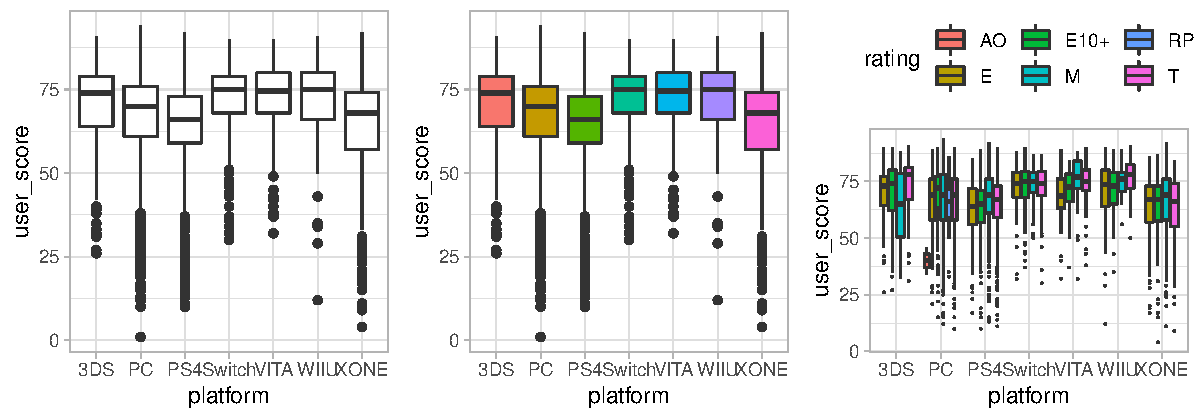
\includegraphics[width=0.9\linewidth]{41-Szinek_files/figure-latex/unnamed-chunk-17-1} \end{center}

\begin{Shaded}
\begin{Highlighting}[]
\FunctionTok{par}\NormalTok{(}\AttributeTok{mfrow =} \FunctionTok{c}\NormalTok{(}\DecValTok{1}\NormalTok{, }\DecValTok{2}\NormalTok{))}
\FunctionTok{barplot}\NormalTok{(x[}\DecValTok{1}\SpecialCharTok{:}\DecValTok{9}\NormalTok{], }\AttributeTok{col =} \FunctionTok{brewer.pal}\NormalTok{(}\AttributeTok{n =} \DecValTok{9}\NormalTok{, }\AttributeTok{name =} \StringTok{"Pastel1"}\NormalTok{), }\AttributeTok{names.arg =} \DecValTok{1}\SpecialCharTok{:}\DecValTok{9}\NormalTok{, }
    \AttributeTok{main =} \StringTok{"Pastel1, qual"}\NormalTok{)}
\FunctionTok{barplot}\NormalTok{(x[}\DecValTok{1}\SpecialCharTok{:}\DecValTok{9}\NormalTok{], }\AttributeTok{col =} \FunctionTok{brewer.pal}\NormalTok{(}\AttributeTok{n =} \DecValTok{9}\NormalTok{, }\AttributeTok{name =} \StringTok{"Pastel1"}\NormalTok{), }\AttributeTok{names.arg =} \DecValTok{1}\SpecialCharTok{:}\DecValTok{9}\NormalTok{, }
    \AttributeTok{main =} \StringTok{"Pastel1, qual"}\NormalTok{, }\AttributeTok{border =} \ConstantTok{NA}\NormalTok{)}
\end{Highlighting}
\end{Shaded}

\begin{center}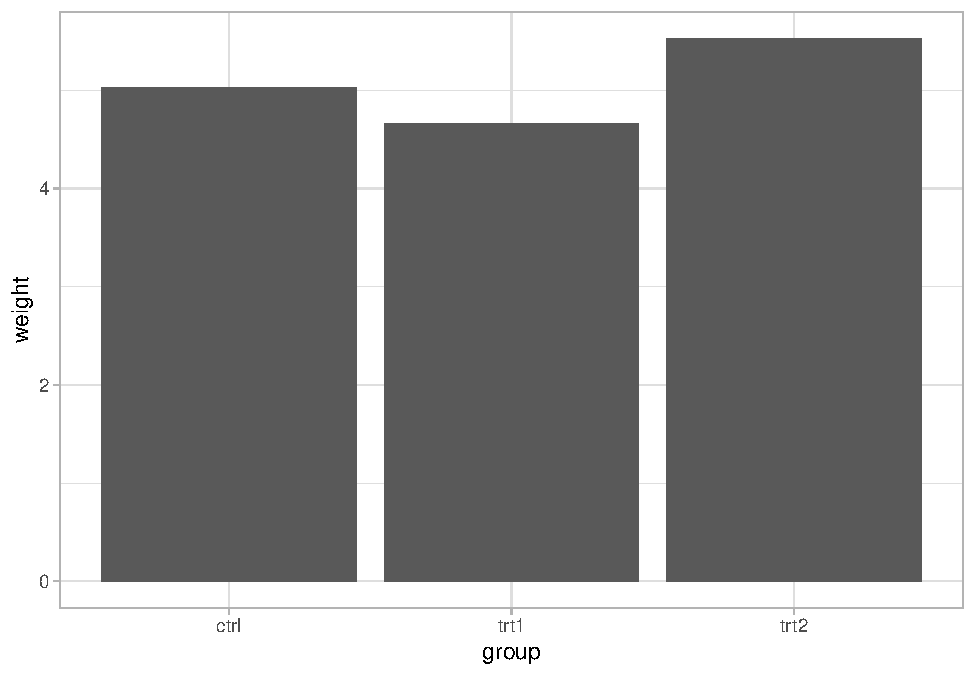
\includegraphics[width=0.9\linewidth]{41-Szinek_files/figure-latex/unnamed-chunk-18-1} \end{center}

\begin{Shaded}
\begin{Highlighting}[]
\FunctionTok{par}\NormalTok{(}\AttributeTok{mfrow =} \FunctionTok{c}\NormalTok{(}\DecValTok{1}\NormalTok{, }\DecValTok{2}\NormalTok{))}
\FunctionTok{barplot}\NormalTok{(x[}\DecValTok{1}\SpecialCharTok{:}\DecValTok{8}\NormalTok{], }\AttributeTok{col =} \FunctionTok{brewer.pal}\NormalTok{(}\AttributeTok{n =} \DecValTok{8}\NormalTok{, }\AttributeTok{name =} \StringTok{"Pastel2"}\NormalTok{), }\AttributeTok{names.arg =} \DecValTok{1}\SpecialCharTok{:}\DecValTok{8}\NormalTok{, }
    \AttributeTok{main =} \StringTok{"Pastel2, qual"}\NormalTok{)}
\FunctionTok{barplot}\NormalTok{(x[}\DecValTok{1}\SpecialCharTok{:}\DecValTok{8}\NormalTok{], }\AttributeTok{col =} \FunctionTok{brewer.pal}\NormalTok{(}\AttributeTok{n =} \DecValTok{8}\NormalTok{, }\AttributeTok{name =} \StringTok{"Pastel2"}\NormalTok{), }\AttributeTok{names.arg =} \DecValTok{1}\SpecialCharTok{:}\DecValTok{8}\NormalTok{, }
    \AttributeTok{main =} \StringTok{"Pastel2, qual"}\NormalTok{, }\AttributeTok{border =} \ConstantTok{NA}\NormalTok{)}
\end{Highlighting}
\end{Shaded}

\begin{center}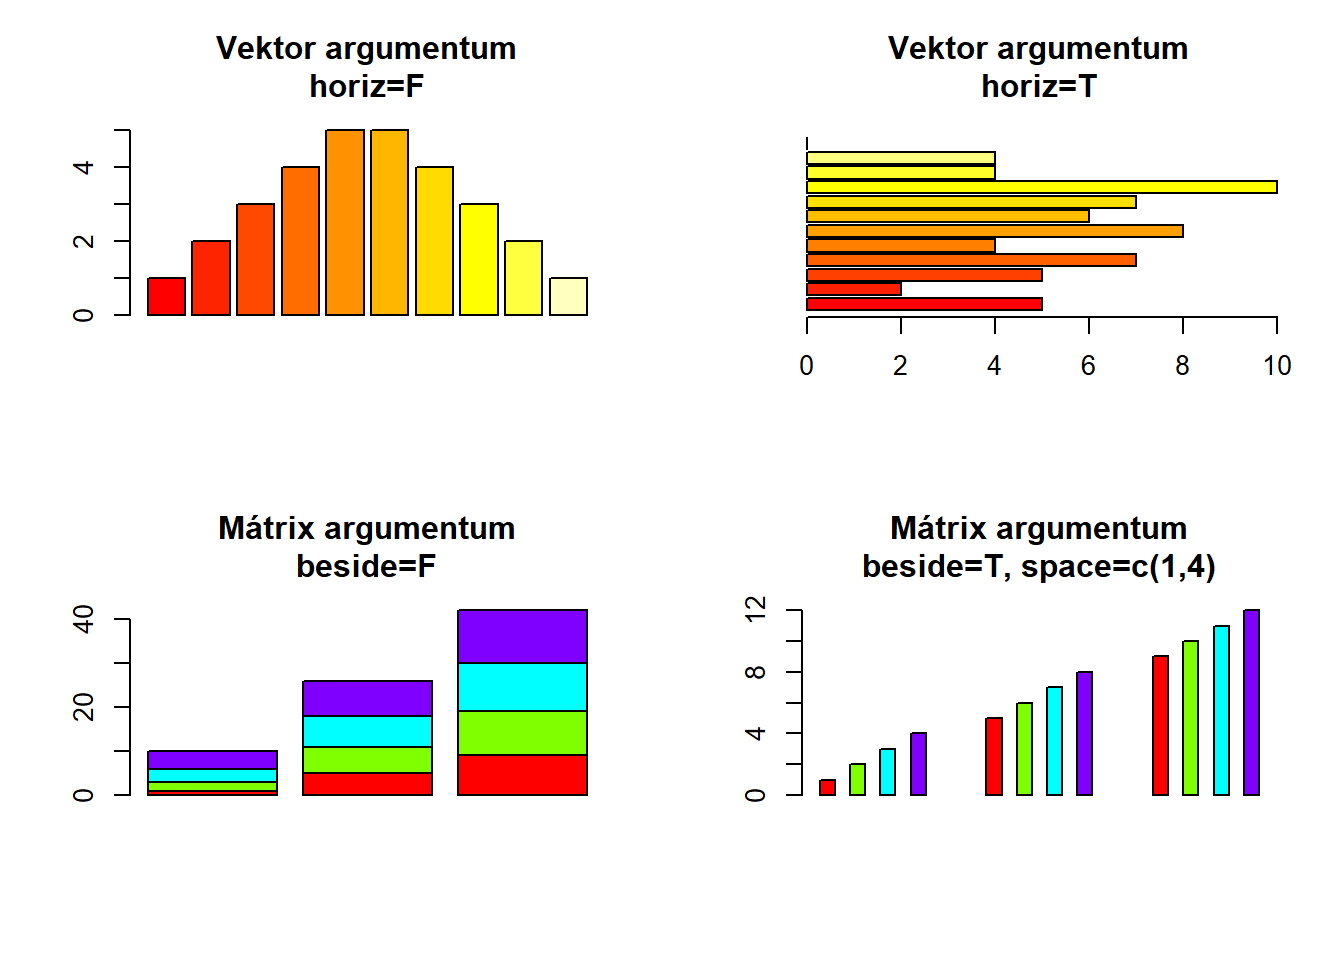
\includegraphics[width=0.9\linewidth]{41-Szinek_files/figure-latex/unnamed-chunk-19-1} \end{center}

\begin{Shaded}
\begin{Highlighting}[]
\FunctionTok{par}\NormalTok{(}\AttributeTok{mfrow =} \FunctionTok{c}\NormalTok{(}\DecValTok{1}\NormalTok{, }\DecValTok{2}\NormalTok{))}
\FunctionTok{barplot}\NormalTok{(x[}\DecValTok{1}\SpecialCharTok{:}\DecValTok{9}\NormalTok{], }\AttributeTok{col =} \FunctionTok{brewer.pal}\NormalTok{(}\AttributeTok{n =} \DecValTok{9}\NormalTok{, }\AttributeTok{name =} \StringTok{"Set1"}\NormalTok{), }\AttributeTok{names.arg =} \DecValTok{1}\SpecialCharTok{:}\DecValTok{9}\NormalTok{, }\AttributeTok{main =} \StringTok{"Set1, qual"}\NormalTok{)}
\FunctionTok{barplot}\NormalTok{(x[}\DecValTok{1}\SpecialCharTok{:}\DecValTok{9}\NormalTok{], }\AttributeTok{col =} \FunctionTok{brewer.pal}\NormalTok{(}\AttributeTok{n =} \DecValTok{9}\NormalTok{, }\AttributeTok{name =} \StringTok{"Set1"}\NormalTok{), }\AttributeTok{names.arg =} \DecValTok{1}\SpecialCharTok{:}\DecValTok{9}\NormalTok{, }\AttributeTok{main =} \StringTok{"Set1, qual"}\NormalTok{, }
    \AttributeTok{border =} \ConstantTok{NA}\NormalTok{)}
\end{Highlighting}
\end{Shaded}

\begin{center}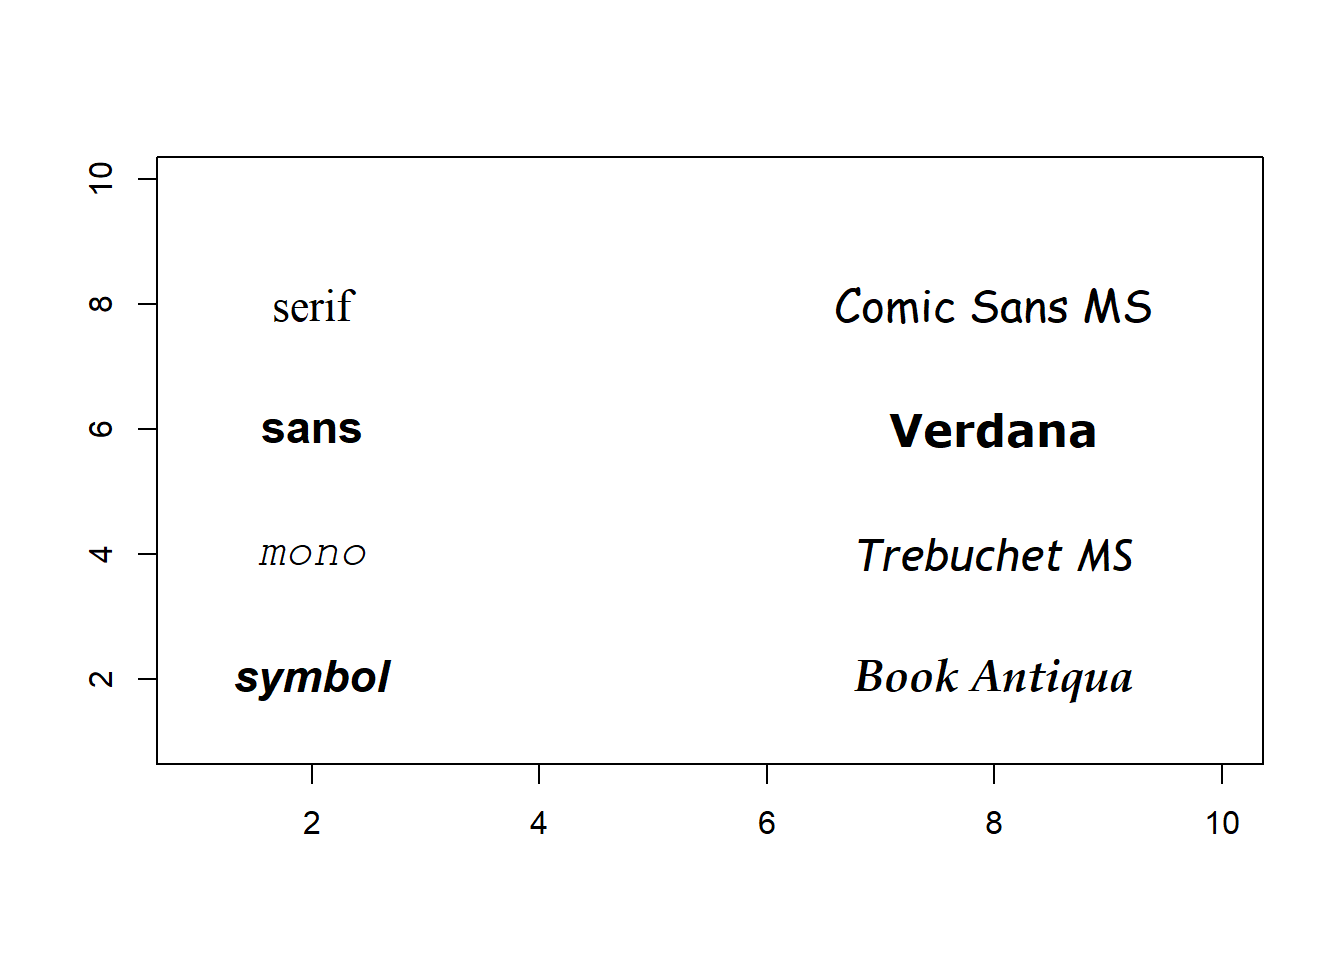
\includegraphics[width=0.9\linewidth]{41-Szinek_files/figure-latex/unnamed-chunk-20-1} \end{center}

\begin{Shaded}
\begin{Highlighting}[]
\FunctionTok{par}\NormalTok{(}\AttributeTok{mfrow =} \FunctionTok{c}\NormalTok{(}\DecValTok{1}\NormalTok{, }\DecValTok{2}\NormalTok{))}
\FunctionTok{barplot}\NormalTok{(x[}\DecValTok{1}\SpecialCharTok{:}\DecValTok{8}\NormalTok{], }\AttributeTok{col =} \FunctionTok{brewer.pal}\NormalTok{(}\AttributeTok{n =} \DecValTok{8}\NormalTok{, }\AttributeTok{name =} \StringTok{"Set2"}\NormalTok{), }\AttributeTok{names.arg =} \DecValTok{1}\SpecialCharTok{:}\DecValTok{8}\NormalTok{, }\AttributeTok{main =} \StringTok{"Set2, qual"}\NormalTok{)}
\FunctionTok{barplot}\NormalTok{(x[}\DecValTok{1}\SpecialCharTok{:}\DecValTok{8}\NormalTok{], }\AttributeTok{col =} \FunctionTok{brewer.pal}\NormalTok{(}\AttributeTok{n =} \DecValTok{8}\NormalTok{, }\AttributeTok{name =} \StringTok{"Set2"}\NormalTok{), }\AttributeTok{names.arg =} \DecValTok{1}\SpecialCharTok{:}\DecValTok{8}\NormalTok{, }\AttributeTok{main =} \StringTok{"Set2, qual"}\NormalTok{, }
    \AttributeTok{border =} \ConstantTok{NA}\NormalTok{)}
\end{Highlighting}
\end{Shaded}

\begin{center}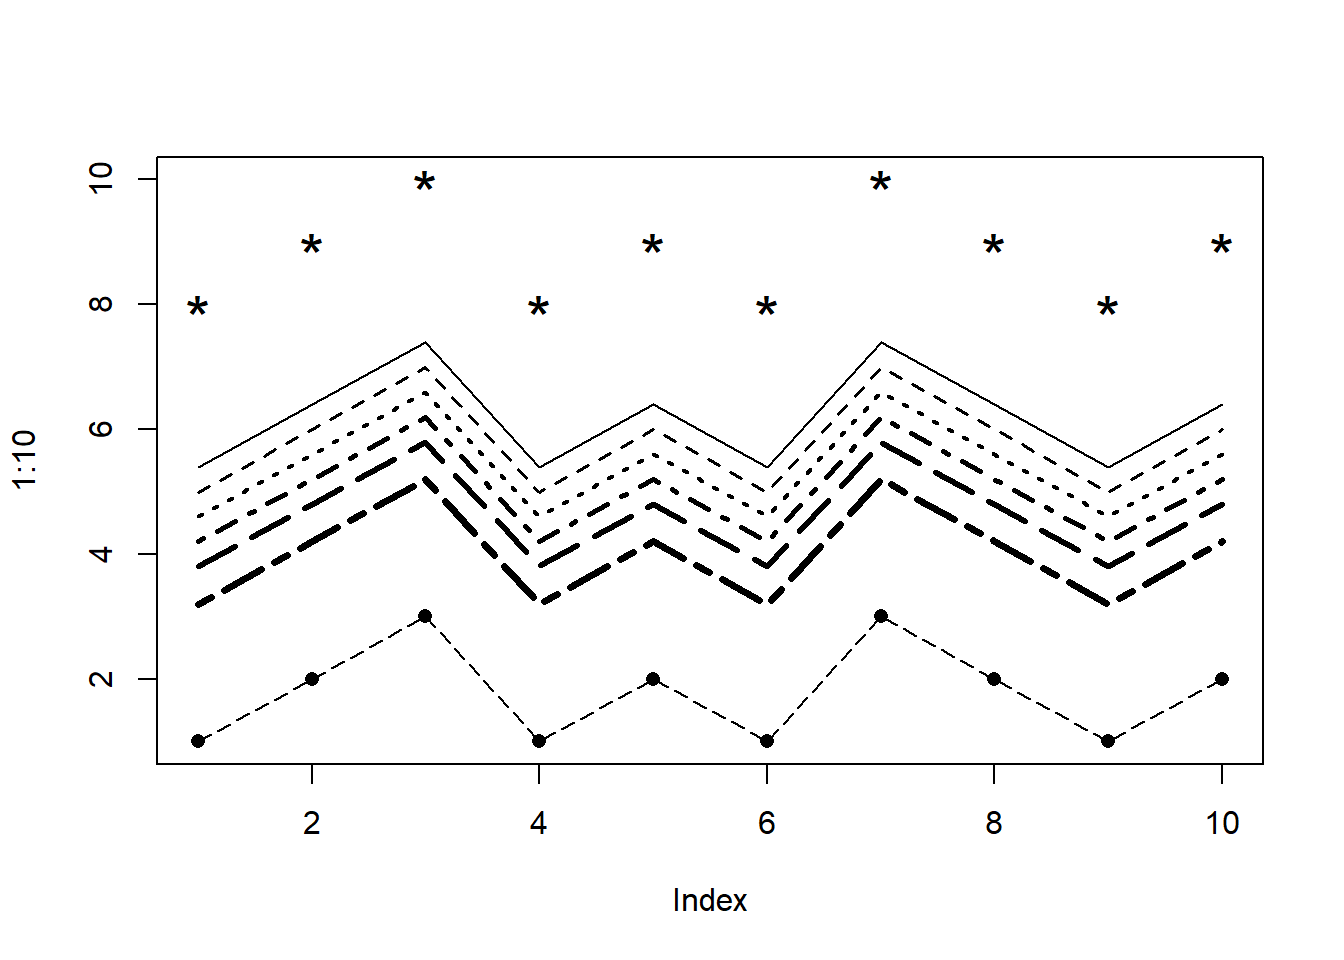
\includegraphics[width=0.9\linewidth]{41-Szinek_files/figure-latex/unnamed-chunk-21-1} \end{center}

\begin{Shaded}
\begin{Highlighting}[]
\FunctionTok{par}\NormalTok{(}\AttributeTok{mfrow =} \FunctionTok{c}\NormalTok{(}\DecValTok{1}\NormalTok{, }\DecValTok{2}\NormalTok{))}
\FunctionTok{barplot}\NormalTok{(x[}\DecValTok{1}\SpecialCharTok{:}\DecValTok{12}\NormalTok{], }\AttributeTok{col =} \FunctionTok{brewer.pal}\NormalTok{(}\AttributeTok{n =} \DecValTok{12}\NormalTok{, }\AttributeTok{name =} \StringTok{"Set3"}\NormalTok{), }\AttributeTok{names.arg =} \DecValTok{1}\SpecialCharTok{:}\DecValTok{12}\NormalTok{, }
    \AttributeTok{main =} \StringTok{"Set3, qual"}\NormalTok{)}
\FunctionTok{barplot}\NormalTok{(x[}\DecValTok{1}\SpecialCharTok{:}\DecValTok{12}\NormalTok{], }\AttributeTok{col =} \FunctionTok{brewer.pal}\NormalTok{(}\AttributeTok{n =} \DecValTok{12}\NormalTok{, }\AttributeTok{name =} \StringTok{"Set3"}\NormalTok{), }\AttributeTok{names.arg =} \DecValTok{1}\SpecialCharTok{:}\DecValTok{12}\NormalTok{, }
    \AttributeTok{main =} \StringTok{"Set3, qual"}\NormalTok{, }\AttributeTok{border =} \ConstantTok{NA}\NormalTok{)}
\end{Highlighting}
\end{Shaded}

\begin{center}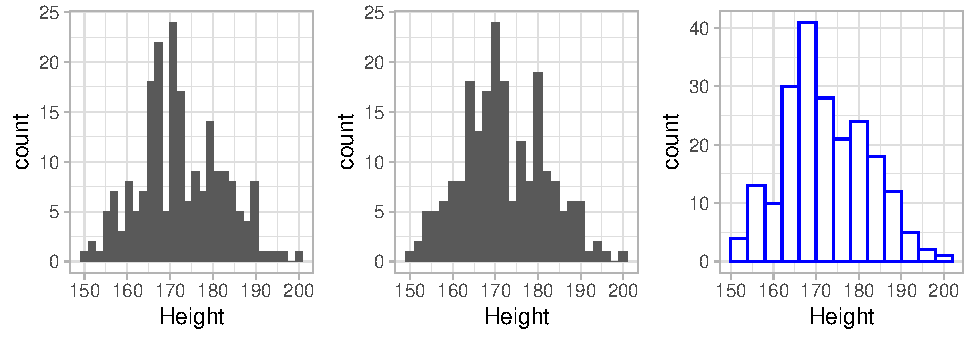
\includegraphics[width=0.9\linewidth]{41-Szinek_files/figure-latex/unnamed-chunk-22-1} \end{center}

\begin{Shaded}
\begin{Highlighting}[]
\FunctionTok{par}\NormalTok{(}\AttributeTok{mfrow =} \FunctionTok{c}\NormalTok{(}\DecValTok{1}\NormalTok{, }\DecValTok{2}\NormalTok{))}
\FunctionTok{barplot}\NormalTok{(x[}\DecValTok{1}\SpecialCharTok{:}\DecValTok{9}\NormalTok{], }\AttributeTok{col =} \FunctionTok{brewer.pal}\NormalTok{(}\AttributeTok{n =} \DecValTok{9}\NormalTok{, }\AttributeTok{name =} \StringTok{"Blues"}\NormalTok{), }\AttributeTok{names.arg =} \DecValTok{1}\SpecialCharTok{:}\DecValTok{9}\NormalTok{, }\AttributeTok{main =} \StringTok{"Blues, seq"}\NormalTok{)}
\FunctionTok{barplot}\NormalTok{(x[}\DecValTok{1}\SpecialCharTok{:}\DecValTok{9}\NormalTok{], }\AttributeTok{col =} \FunctionTok{brewer.pal}\NormalTok{(}\AttributeTok{n =} \DecValTok{9}\NormalTok{, }\AttributeTok{name =} \StringTok{"Blues"}\NormalTok{), }\AttributeTok{names.arg =} \DecValTok{1}\SpecialCharTok{:}\DecValTok{9}\NormalTok{, }\AttributeTok{main =} \StringTok{"Blues, seq"}\NormalTok{, }
    \AttributeTok{border =} \ConstantTok{NA}\NormalTok{)}
\end{Highlighting}
\end{Shaded}

\begin{center}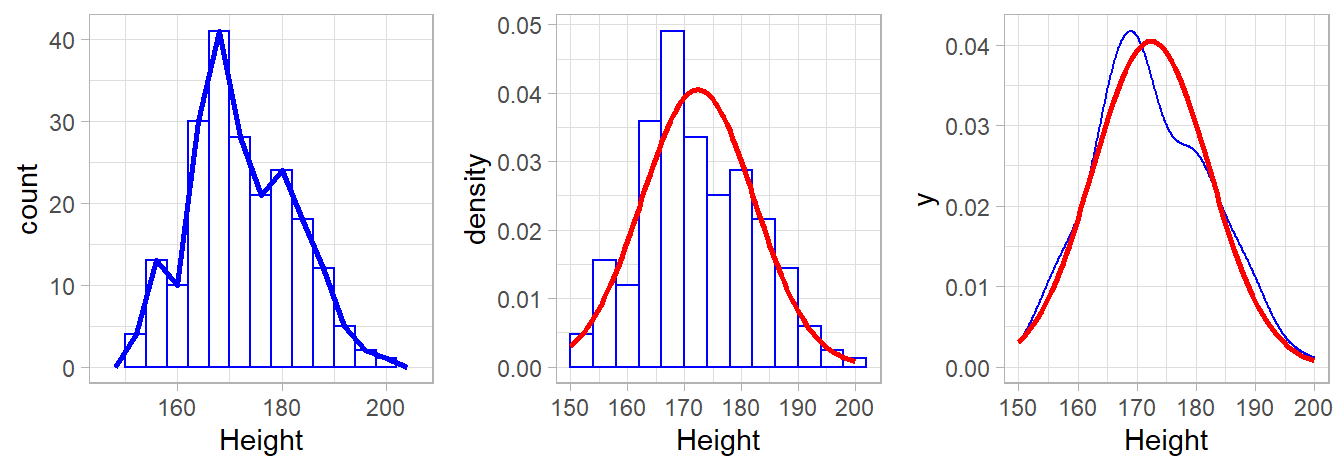
\includegraphics[width=0.9\linewidth]{41-Szinek_files/figure-latex/unnamed-chunk-23-1} \end{center}

\begin{Shaded}
\begin{Highlighting}[]
\FunctionTok{par}\NormalTok{(}\AttributeTok{mfrow =} \FunctionTok{c}\NormalTok{(}\DecValTok{1}\NormalTok{, }\DecValTok{2}\NormalTok{))}
\FunctionTok{barplot}\NormalTok{(x[}\DecValTok{1}\SpecialCharTok{:}\DecValTok{9}\NormalTok{], }\AttributeTok{col =} \FunctionTok{brewer.pal}\NormalTok{(}\AttributeTok{n =} \DecValTok{9}\NormalTok{, }\AttributeTok{name =} \StringTok{"BuGn"}\NormalTok{), }\AttributeTok{names.arg =} \DecValTok{1}\SpecialCharTok{:}\DecValTok{9}\NormalTok{, }\AttributeTok{main =} \StringTok{"BuGn, seq"}\NormalTok{)}
\FunctionTok{barplot}\NormalTok{(x[}\DecValTok{1}\SpecialCharTok{:}\DecValTok{9}\NormalTok{], }\AttributeTok{col =} \FunctionTok{brewer.pal}\NormalTok{(}\AttributeTok{n =} \DecValTok{9}\NormalTok{, }\AttributeTok{name =} \StringTok{"BuGn"}\NormalTok{), }\AttributeTok{names.arg =} \DecValTok{1}\SpecialCharTok{:}\DecValTok{9}\NormalTok{, }\AttributeTok{main =} \StringTok{"BuGn, seq"}\NormalTok{, }
    \AttributeTok{border =} \ConstantTok{NA}\NormalTok{)}
\end{Highlighting}
\end{Shaded}

\begin{center}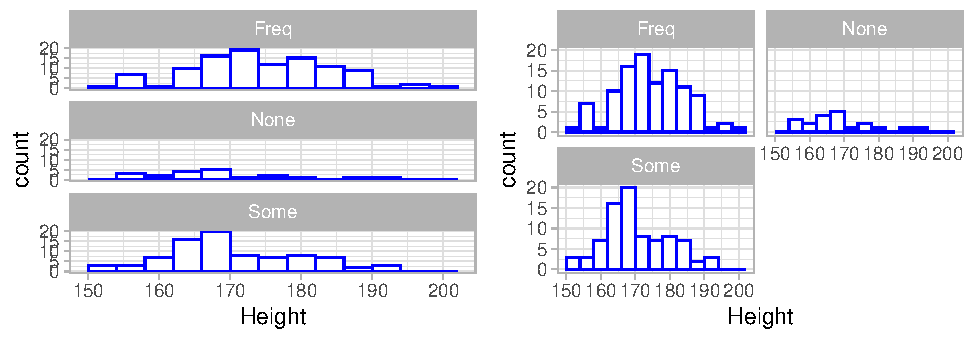
\includegraphics[width=0.9\linewidth]{41-Szinek_files/figure-latex/unnamed-chunk-24-1} \end{center}

\begin{Shaded}
\begin{Highlighting}[]
\FunctionTok{par}\NormalTok{(}\AttributeTok{mfrow =} \FunctionTok{c}\NormalTok{(}\DecValTok{1}\NormalTok{, }\DecValTok{2}\NormalTok{))}
\FunctionTok{barplot}\NormalTok{(x[}\DecValTok{1}\SpecialCharTok{:}\DecValTok{9}\NormalTok{], }\AttributeTok{col =} \FunctionTok{brewer.pal}\NormalTok{(}\AttributeTok{n =} \DecValTok{9}\NormalTok{, }\AttributeTok{name =} \StringTok{"BuPu"}\NormalTok{), }\AttributeTok{names.arg =} \DecValTok{1}\SpecialCharTok{:}\DecValTok{9}\NormalTok{, }\AttributeTok{main =} \StringTok{"BuPu, seq"}\NormalTok{)}
\FunctionTok{barplot}\NormalTok{(x[}\DecValTok{1}\SpecialCharTok{:}\DecValTok{9}\NormalTok{], }\AttributeTok{col =} \FunctionTok{brewer.pal}\NormalTok{(}\AttributeTok{n =} \DecValTok{9}\NormalTok{, }\AttributeTok{name =} \StringTok{"BuPu"}\NormalTok{), }\AttributeTok{names.arg =} \DecValTok{1}\SpecialCharTok{:}\DecValTok{9}\NormalTok{, }\AttributeTok{main =} \StringTok{"BuPu, seq"}\NormalTok{, }
    \AttributeTok{border =} \ConstantTok{NA}\NormalTok{)}
\end{Highlighting}
\end{Shaded}

\begin{center}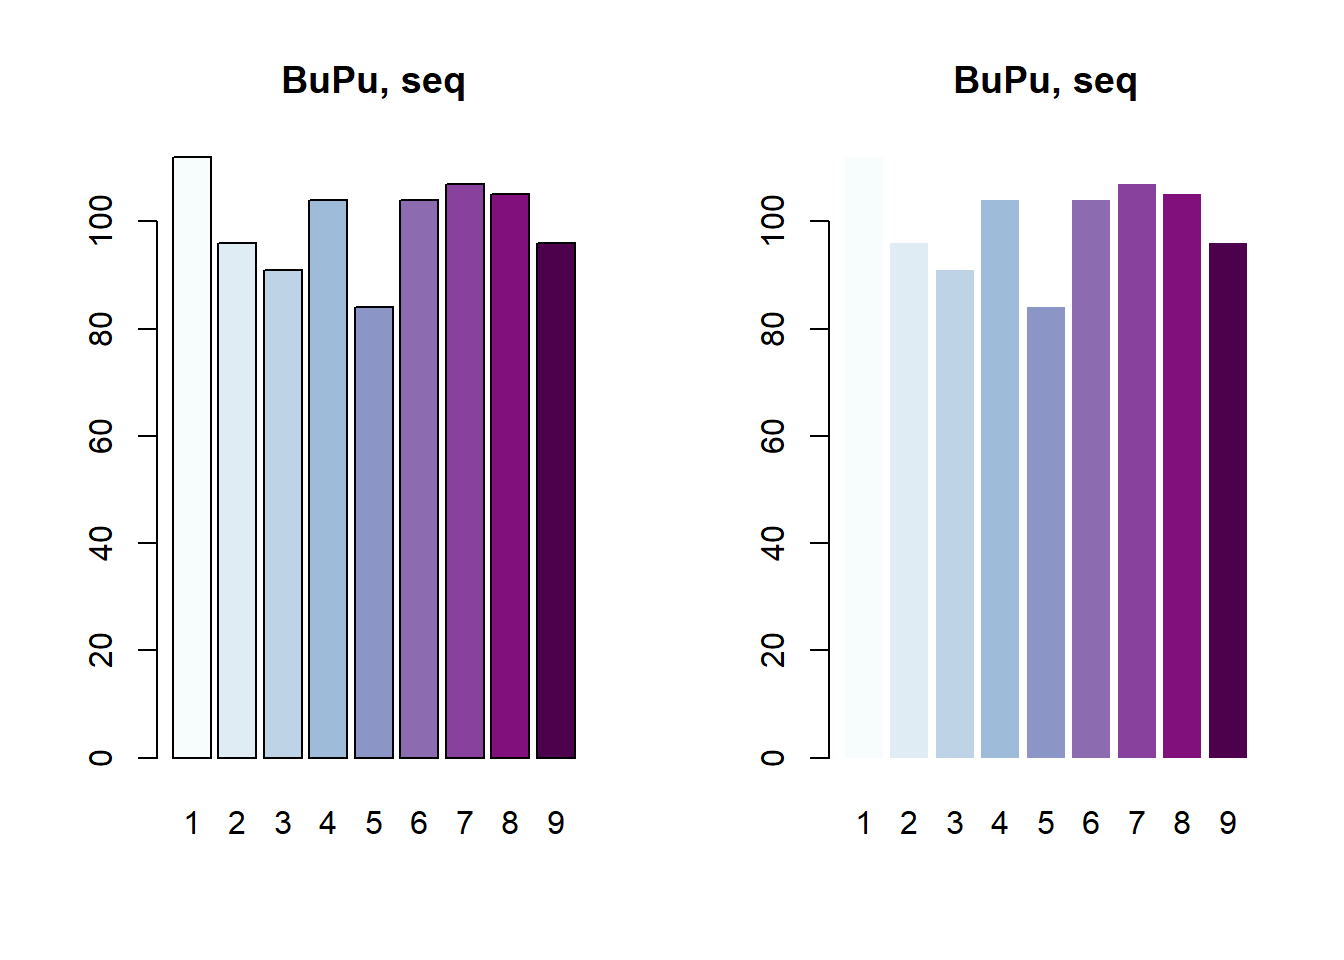
\includegraphics[width=0.9\linewidth]{41-Szinek_files/figure-latex/unnamed-chunk-25-1} \end{center}

\begin{Shaded}
\begin{Highlighting}[]
\FunctionTok{par}\NormalTok{(}\AttributeTok{mfrow =} \FunctionTok{c}\NormalTok{(}\DecValTok{1}\NormalTok{, }\DecValTok{2}\NormalTok{))}
\FunctionTok{barplot}\NormalTok{(x[}\DecValTok{1}\SpecialCharTok{:}\DecValTok{9}\NormalTok{], }\AttributeTok{col =} \FunctionTok{brewer.pal}\NormalTok{(}\AttributeTok{n =} \DecValTok{9}\NormalTok{, }\AttributeTok{name =} \StringTok{"GnBu"}\NormalTok{), }\AttributeTok{names.arg =} \DecValTok{1}\SpecialCharTok{:}\DecValTok{9}\NormalTok{, }\AttributeTok{main =} \StringTok{"GnBu, seq"}\NormalTok{)}
\FunctionTok{barplot}\NormalTok{(x[}\DecValTok{1}\SpecialCharTok{:}\DecValTok{9}\NormalTok{], }\AttributeTok{col =} \FunctionTok{brewer.pal}\NormalTok{(}\AttributeTok{n =} \DecValTok{9}\NormalTok{, }\AttributeTok{name =} \StringTok{"GnBu"}\NormalTok{), }\AttributeTok{names.arg =} \DecValTok{1}\SpecialCharTok{:}\DecValTok{9}\NormalTok{, }\AttributeTok{main =} \StringTok{"GnBu, seq"}\NormalTok{, }
    \AttributeTok{border =} \ConstantTok{NA}\NormalTok{)}
\end{Highlighting}
\end{Shaded}

\begin{center}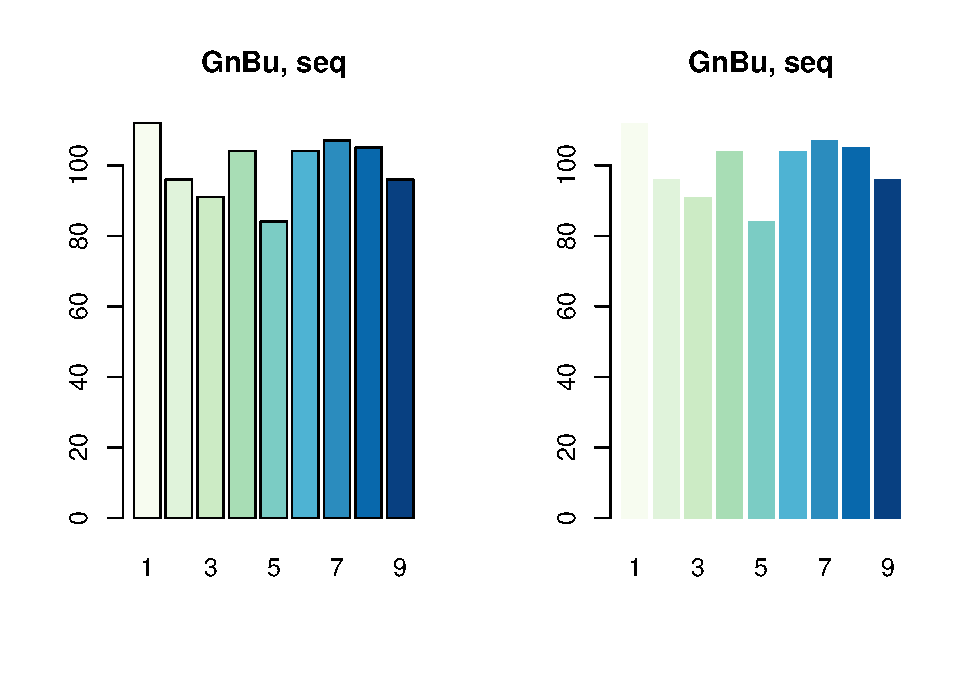
\includegraphics[width=0.9\linewidth]{41-Szinek_files/figure-latex/unnamed-chunk-26-1} \end{center}

\begin{Shaded}
\begin{Highlighting}[]
\FunctionTok{par}\NormalTok{(}\AttributeTok{mfrow =} \FunctionTok{c}\NormalTok{(}\DecValTok{1}\NormalTok{, }\DecValTok{2}\NormalTok{))}
\FunctionTok{barplot}\NormalTok{(x[}\DecValTok{1}\SpecialCharTok{:}\DecValTok{9}\NormalTok{], }\AttributeTok{col =} \FunctionTok{brewer.pal}\NormalTok{(}\AttributeTok{n =} \DecValTok{9}\NormalTok{, }\AttributeTok{name =} \StringTok{"Greens"}\NormalTok{), }\AttributeTok{names.arg =} \DecValTok{1}\SpecialCharTok{:}\DecValTok{9}\NormalTok{, }\AttributeTok{main =} \StringTok{"Greens, seq"}\NormalTok{)}
\FunctionTok{barplot}\NormalTok{(x[}\DecValTok{1}\SpecialCharTok{:}\DecValTok{9}\NormalTok{], }\AttributeTok{col =} \FunctionTok{brewer.pal}\NormalTok{(}\AttributeTok{n =} \DecValTok{9}\NormalTok{, }\AttributeTok{name =} \StringTok{"Greens"}\NormalTok{), }\AttributeTok{names.arg =} \DecValTok{1}\SpecialCharTok{:}\DecValTok{9}\NormalTok{, }\AttributeTok{main =} \StringTok{"Greens, seq"}\NormalTok{, }
    \AttributeTok{border =} \ConstantTok{NA}\NormalTok{)}
\end{Highlighting}
\end{Shaded}

\begin{center}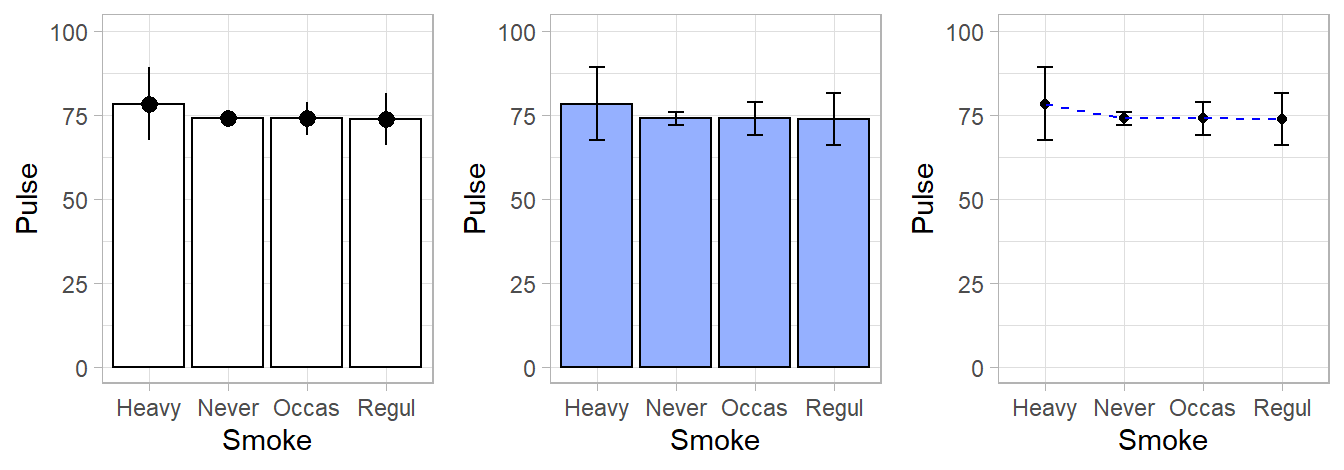
\includegraphics[width=0.9\linewidth]{41-Szinek_files/figure-latex/unnamed-chunk-27-1} \end{center}

\begin{Shaded}
\begin{Highlighting}[]
\FunctionTok{par}\NormalTok{(}\AttributeTok{mfrow =} \FunctionTok{c}\NormalTok{(}\DecValTok{1}\NormalTok{, }\DecValTok{2}\NormalTok{))}
\FunctionTok{barplot}\NormalTok{(x[}\DecValTok{1}\SpecialCharTok{:}\DecValTok{9}\NormalTok{], }\AttributeTok{col =} \FunctionTok{brewer.pal}\NormalTok{(}\AttributeTok{n =} \DecValTok{9}\NormalTok{, }\AttributeTok{name =} \StringTok{"Greys"}\NormalTok{), }\AttributeTok{names.arg =} \DecValTok{1}\SpecialCharTok{:}\DecValTok{9}\NormalTok{, }\AttributeTok{main =} \StringTok{"Greys, seq"}\NormalTok{)}
\FunctionTok{barplot}\NormalTok{(x[}\DecValTok{1}\SpecialCharTok{:}\DecValTok{9}\NormalTok{], }\AttributeTok{col =} \FunctionTok{brewer.pal}\NormalTok{(}\AttributeTok{n =} \DecValTok{9}\NormalTok{, }\AttributeTok{name =} \StringTok{"Greys"}\NormalTok{), }\AttributeTok{names.arg =} \DecValTok{1}\SpecialCharTok{:}\DecValTok{9}\NormalTok{, }\AttributeTok{main =} \StringTok{"Greys, seq"}\NormalTok{, }
    \AttributeTok{border =} \ConstantTok{NA}\NormalTok{)}
\end{Highlighting}
\end{Shaded}

\begin{center}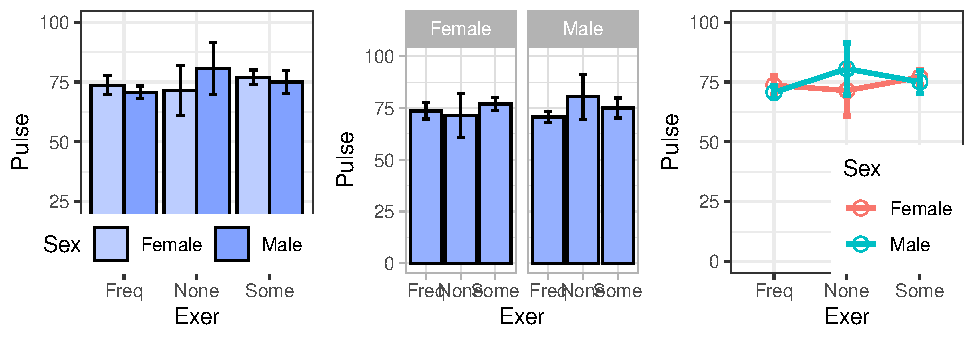
\includegraphics[width=0.9\linewidth]{41-Szinek_files/figure-latex/unnamed-chunk-28-1} \end{center}

\begin{Shaded}
\begin{Highlighting}[]
\FunctionTok{par}\NormalTok{(}\AttributeTok{mfrow =} \FunctionTok{c}\NormalTok{(}\DecValTok{1}\NormalTok{, }\DecValTok{2}\NormalTok{))}
\FunctionTok{barplot}\NormalTok{(x[}\DecValTok{1}\SpecialCharTok{:}\DecValTok{9}\NormalTok{], }\AttributeTok{col =} \FunctionTok{brewer.pal}\NormalTok{(}\AttributeTok{n =} \DecValTok{9}\NormalTok{, }\AttributeTok{name =} \StringTok{"Oranges"}\NormalTok{), }\AttributeTok{names.arg =} \DecValTok{1}\SpecialCharTok{:}\DecValTok{9}\NormalTok{, }
    \AttributeTok{main =} \StringTok{"Oranges, seq"}\NormalTok{)}
\FunctionTok{barplot}\NormalTok{(x[}\DecValTok{1}\SpecialCharTok{:}\DecValTok{9}\NormalTok{], }\AttributeTok{col =} \FunctionTok{brewer.pal}\NormalTok{(}\AttributeTok{n =} \DecValTok{9}\NormalTok{, }\AttributeTok{name =} \StringTok{"Oranges"}\NormalTok{), }\AttributeTok{names.arg =} \DecValTok{1}\SpecialCharTok{:}\DecValTok{9}\NormalTok{, }
    \AttributeTok{main =} \StringTok{"Oranges, seq"}\NormalTok{, }\AttributeTok{border =} \ConstantTok{NA}\NormalTok{)}
\end{Highlighting}
\end{Shaded}

\begin{center}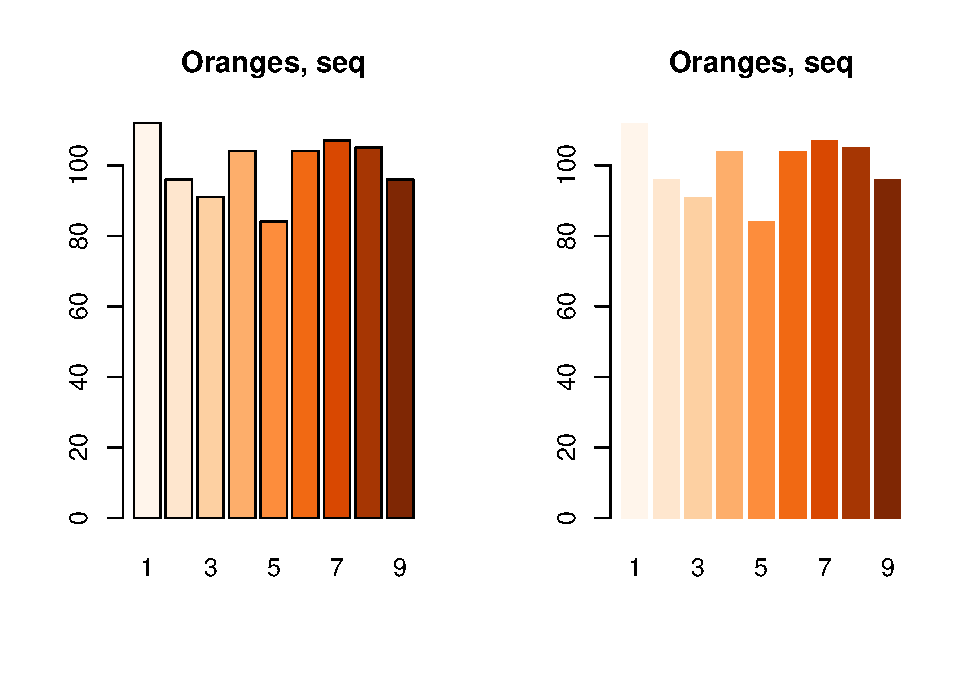
\includegraphics[width=0.9\linewidth]{41-Szinek_files/figure-latex/unnamed-chunk-29-1} \end{center}

\begin{Shaded}
\begin{Highlighting}[]
\FunctionTok{par}\NormalTok{(}\AttributeTok{mfrow =} \FunctionTok{c}\NormalTok{(}\DecValTok{1}\NormalTok{, }\DecValTok{2}\NormalTok{))}
\FunctionTok{barplot}\NormalTok{(x[}\DecValTok{1}\SpecialCharTok{:}\DecValTok{9}\NormalTok{], }\AttributeTok{col =} \FunctionTok{brewer.pal}\NormalTok{(}\AttributeTok{n =} \DecValTok{9}\NormalTok{, }\AttributeTok{name =} \StringTok{"OrRd"}\NormalTok{), }\AttributeTok{names.arg =} \DecValTok{1}\SpecialCharTok{:}\DecValTok{9}\NormalTok{, }\AttributeTok{main =} \StringTok{"OrRd, seq"}\NormalTok{)}
\FunctionTok{barplot}\NormalTok{(x[}\DecValTok{1}\SpecialCharTok{:}\DecValTok{9}\NormalTok{], }\AttributeTok{col =} \FunctionTok{brewer.pal}\NormalTok{(}\AttributeTok{n =} \DecValTok{9}\NormalTok{, }\AttributeTok{name =} \StringTok{"OrRd"}\NormalTok{), }\AttributeTok{names.arg =} \DecValTok{1}\SpecialCharTok{:}\DecValTok{9}\NormalTok{, }\AttributeTok{main =} \StringTok{"OrRd, seq"}\NormalTok{, }
    \AttributeTok{border =} \ConstantTok{NA}\NormalTok{)}
\end{Highlighting}
\end{Shaded}

\begin{center}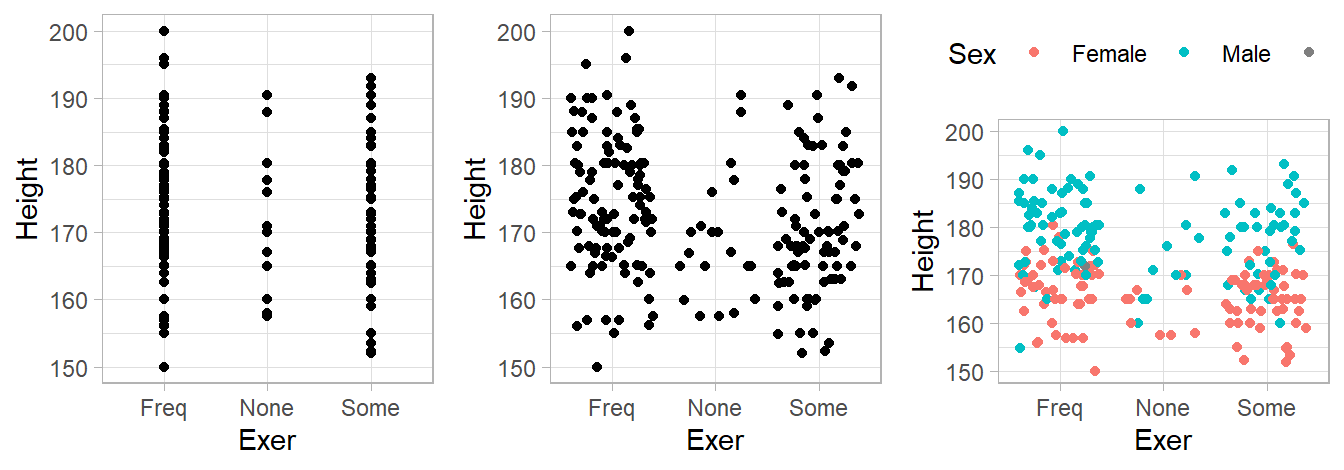
\includegraphics[width=0.9\linewidth]{41-Szinek_files/figure-latex/unnamed-chunk-30-1} \end{center}

\begin{Shaded}
\begin{Highlighting}[]
\FunctionTok{par}\NormalTok{(}\AttributeTok{mfrow =} \FunctionTok{c}\NormalTok{(}\DecValTok{1}\NormalTok{, }\DecValTok{2}\NormalTok{))}
\FunctionTok{barplot}\NormalTok{(x[}\DecValTok{1}\SpecialCharTok{:}\DecValTok{9}\NormalTok{], }\AttributeTok{col =} \FunctionTok{brewer.pal}\NormalTok{(}\AttributeTok{n =} \DecValTok{9}\NormalTok{, }\AttributeTok{name =} \StringTok{"PuBu"}\NormalTok{), }\AttributeTok{names.arg =} \DecValTok{1}\SpecialCharTok{:}\DecValTok{9}\NormalTok{, }\AttributeTok{main =} \StringTok{"PuBu, seq"}\NormalTok{)}
\FunctionTok{barplot}\NormalTok{(x[}\DecValTok{1}\SpecialCharTok{:}\DecValTok{9}\NormalTok{], }\AttributeTok{col =} \FunctionTok{brewer.pal}\NormalTok{(}\AttributeTok{n =} \DecValTok{9}\NormalTok{, }\AttributeTok{name =} \StringTok{"PuBu"}\NormalTok{), }\AttributeTok{names.arg =} \DecValTok{1}\SpecialCharTok{:}\DecValTok{9}\NormalTok{, }\AttributeTok{main =} \StringTok{"PuBu, seq"}\NormalTok{, }
    \AttributeTok{border =} \ConstantTok{NA}\NormalTok{)}
\end{Highlighting}
\end{Shaded}

\begin{center}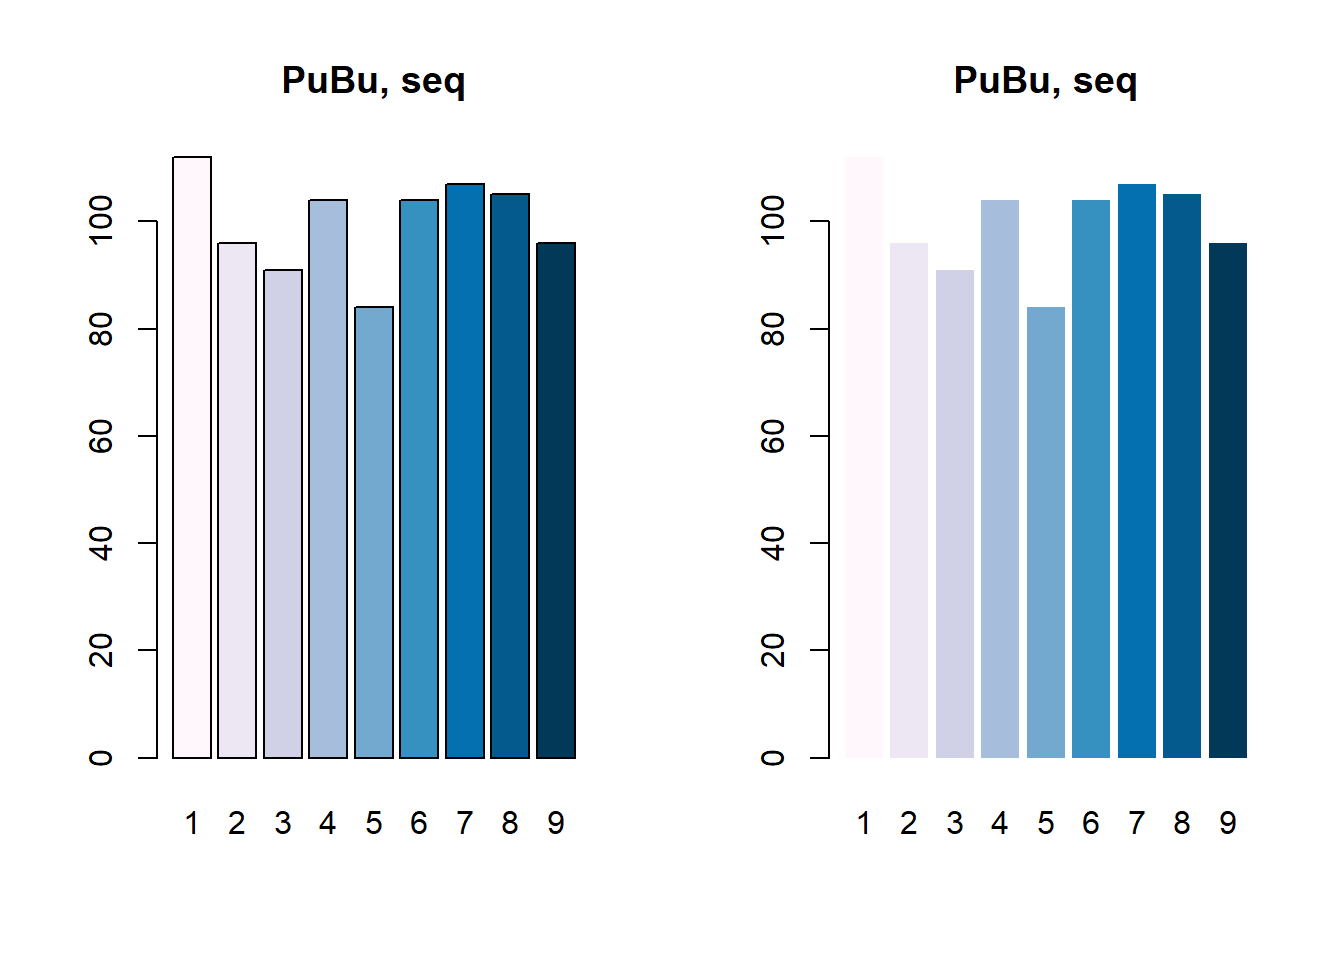
\includegraphics[width=0.9\linewidth]{41-Szinek_files/figure-latex/unnamed-chunk-31-1} \end{center}

\begin{Shaded}
\begin{Highlighting}[]
\FunctionTok{par}\NormalTok{(}\AttributeTok{mfrow =} \FunctionTok{c}\NormalTok{(}\DecValTok{1}\NormalTok{, }\DecValTok{2}\NormalTok{))}
\FunctionTok{barplot}\NormalTok{(x[}\DecValTok{1}\SpecialCharTok{:}\DecValTok{9}\NormalTok{], }\AttributeTok{col =} \FunctionTok{brewer.pal}\NormalTok{(}\AttributeTok{n =} \DecValTok{9}\NormalTok{, }\AttributeTok{name =} \StringTok{"PuBuGn"}\NormalTok{), }\AttributeTok{names.arg =} \DecValTok{1}\SpecialCharTok{:}\DecValTok{9}\NormalTok{, }\AttributeTok{main =} \StringTok{"PuBuGn, seq"}\NormalTok{)}
\FunctionTok{barplot}\NormalTok{(x[}\DecValTok{1}\SpecialCharTok{:}\DecValTok{9}\NormalTok{], }\AttributeTok{col =} \FunctionTok{brewer.pal}\NormalTok{(}\AttributeTok{n =} \DecValTok{9}\NormalTok{, }\AttributeTok{name =} \StringTok{"PuBuGn"}\NormalTok{), }\AttributeTok{names.arg =} \DecValTok{1}\SpecialCharTok{:}\DecValTok{9}\NormalTok{, }\AttributeTok{main =} \StringTok{"PuBuGn, seq"}\NormalTok{, }
    \AttributeTok{border =} \ConstantTok{NA}\NormalTok{)}
\end{Highlighting}
\end{Shaded}

\begin{center}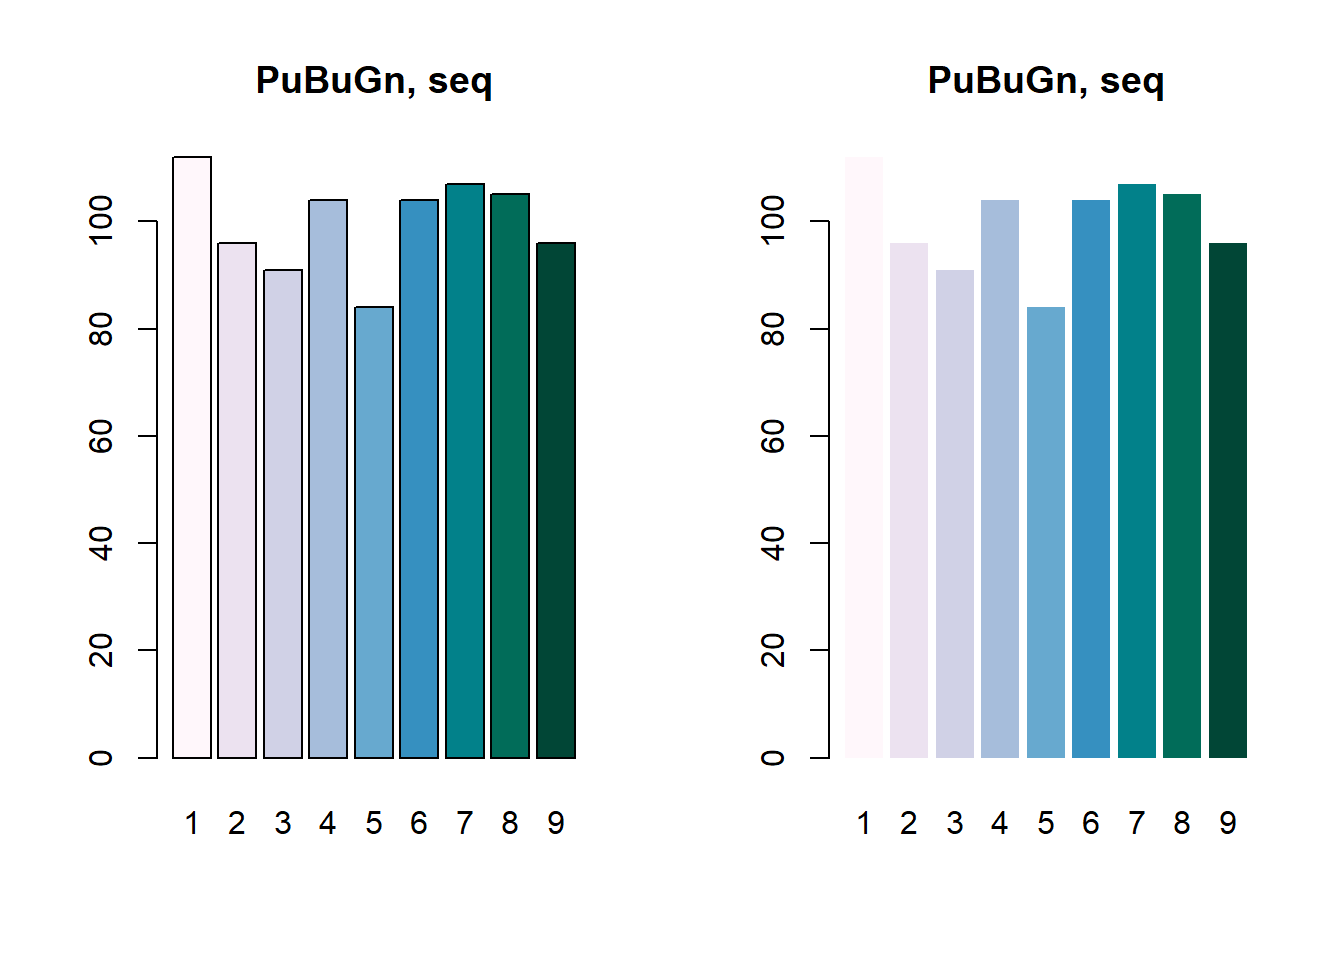
\includegraphics[width=0.9\linewidth]{41-Szinek_files/figure-latex/unnamed-chunk-32-1} \end{center}

\begin{Shaded}
\begin{Highlighting}[]
\FunctionTok{par}\NormalTok{(}\AttributeTok{mfrow =} \FunctionTok{c}\NormalTok{(}\DecValTok{1}\NormalTok{, }\DecValTok{2}\NormalTok{))}
\FunctionTok{barplot}\NormalTok{(x[}\DecValTok{1}\SpecialCharTok{:}\DecValTok{9}\NormalTok{], }\AttributeTok{col =} \FunctionTok{brewer.pal}\NormalTok{(}\AttributeTok{n =} \DecValTok{9}\NormalTok{, }\AttributeTok{name =} \StringTok{"PuRd"}\NormalTok{), }\AttributeTok{names.arg =} \DecValTok{1}\SpecialCharTok{:}\DecValTok{9}\NormalTok{, }\AttributeTok{main =} \StringTok{"PuRd, seq"}\NormalTok{)}
\FunctionTok{barplot}\NormalTok{(x[}\DecValTok{1}\SpecialCharTok{:}\DecValTok{9}\NormalTok{], }\AttributeTok{col =} \FunctionTok{brewer.pal}\NormalTok{(}\AttributeTok{n =} \DecValTok{9}\NormalTok{, }\AttributeTok{name =} \StringTok{"PuRd"}\NormalTok{), }\AttributeTok{names.arg =} \DecValTok{1}\SpecialCharTok{:}\DecValTok{9}\NormalTok{, }\AttributeTok{main =} \StringTok{"PuRd, seq"}\NormalTok{, }
    \AttributeTok{border =} \ConstantTok{NA}\NormalTok{)}
\end{Highlighting}
\end{Shaded}

\begin{center}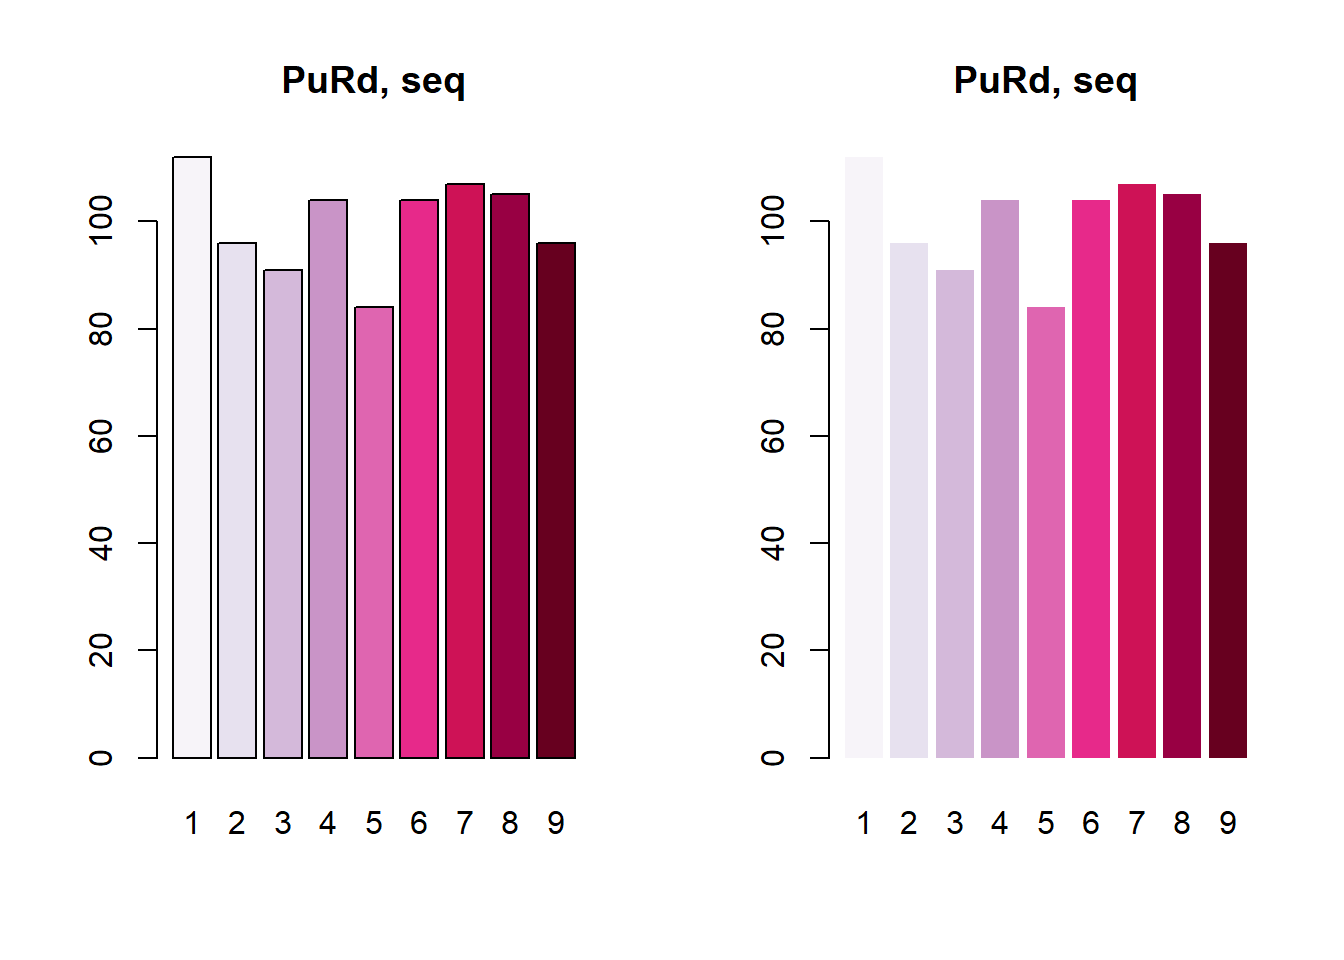
\includegraphics[width=0.9\linewidth]{41-Szinek_files/figure-latex/unnamed-chunk-33-1} \end{center}

\begin{Shaded}
\begin{Highlighting}[]
\FunctionTok{par}\NormalTok{(}\AttributeTok{mfrow =} \FunctionTok{c}\NormalTok{(}\DecValTok{1}\NormalTok{, }\DecValTok{2}\NormalTok{))}
\FunctionTok{barplot}\NormalTok{(x[}\DecValTok{1}\SpecialCharTok{:}\DecValTok{9}\NormalTok{], }\AttributeTok{col =} \FunctionTok{brewer.pal}\NormalTok{(}\AttributeTok{n =} \DecValTok{9}\NormalTok{, }\AttributeTok{name =} \StringTok{"Purples"}\NormalTok{), }\AttributeTok{names.arg =} \DecValTok{1}\SpecialCharTok{:}\DecValTok{9}\NormalTok{, }
    \AttributeTok{main =} \StringTok{"Purples, seq"}\NormalTok{)}
\FunctionTok{barplot}\NormalTok{(x[}\DecValTok{1}\SpecialCharTok{:}\DecValTok{9}\NormalTok{], }\AttributeTok{col =} \FunctionTok{brewer.pal}\NormalTok{(}\AttributeTok{n =} \DecValTok{9}\NormalTok{, }\AttributeTok{name =} \StringTok{"Purples"}\NormalTok{), }\AttributeTok{names.arg =} \DecValTok{1}\SpecialCharTok{:}\DecValTok{9}\NormalTok{, }
    \AttributeTok{main =} \StringTok{"Purples, seq"}\NormalTok{, }\AttributeTok{border =} \ConstantTok{NA}\NormalTok{)}
\end{Highlighting}
\end{Shaded}

\begin{center}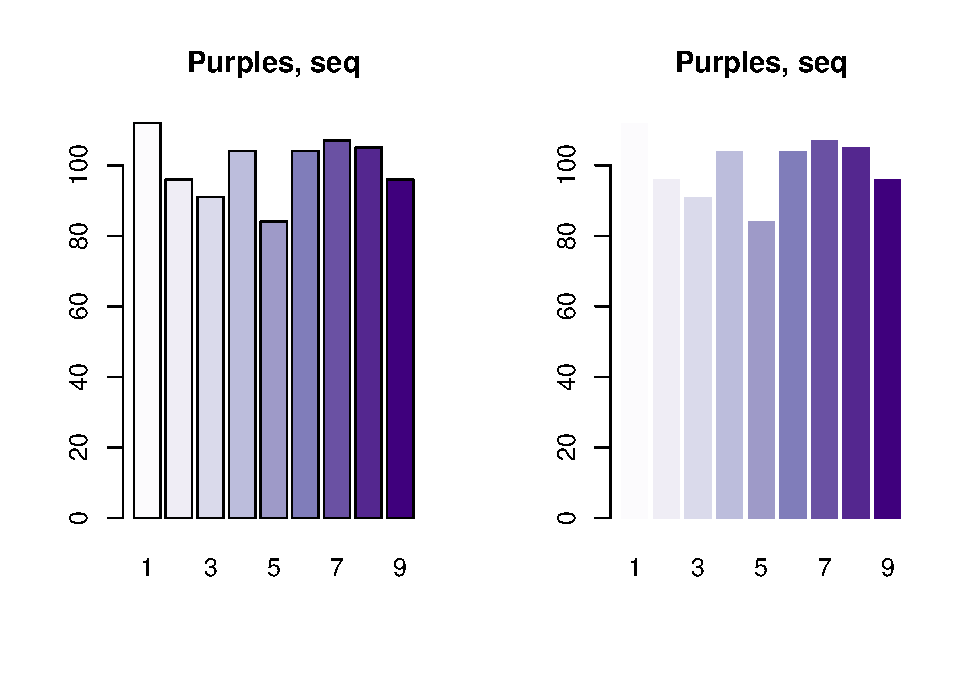
\includegraphics[width=0.9\linewidth]{41-Szinek_files/figure-latex/unnamed-chunk-34-1} \end{center}

\begin{Shaded}
\begin{Highlighting}[]
\FunctionTok{par}\NormalTok{(}\AttributeTok{mfrow =} \FunctionTok{c}\NormalTok{(}\DecValTok{1}\NormalTok{, }\DecValTok{2}\NormalTok{))}
\FunctionTok{barplot}\NormalTok{(x[}\DecValTok{1}\SpecialCharTok{:}\DecValTok{9}\NormalTok{], }\AttributeTok{col =} \FunctionTok{brewer.pal}\NormalTok{(}\AttributeTok{n =} \DecValTok{9}\NormalTok{, }\AttributeTok{name =} \StringTok{"RdPu"}\NormalTok{), }\AttributeTok{names.arg =} \DecValTok{1}\SpecialCharTok{:}\DecValTok{9}\NormalTok{, }\AttributeTok{main =} \StringTok{"RdPu, seq"}\NormalTok{)}
\FunctionTok{barplot}\NormalTok{(x[}\DecValTok{1}\SpecialCharTok{:}\DecValTok{9}\NormalTok{], }\AttributeTok{col =} \FunctionTok{brewer.pal}\NormalTok{(}\AttributeTok{n =} \DecValTok{9}\NormalTok{, }\AttributeTok{name =} \StringTok{"RdPu"}\NormalTok{), }\AttributeTok{names.arg =} \DecValTok{1}\SpecialCharTok{:}\DecValTok{9}\NormalTok{, }\AttributeTok{main =} \StringTok{"RdPu, seq"}\NormalTok{, }
    \AttributeTok{border =} \ConstantTok{NA}\NormalTok{)}
\end{Highlighting}
\end{Shaded}

\begin{center}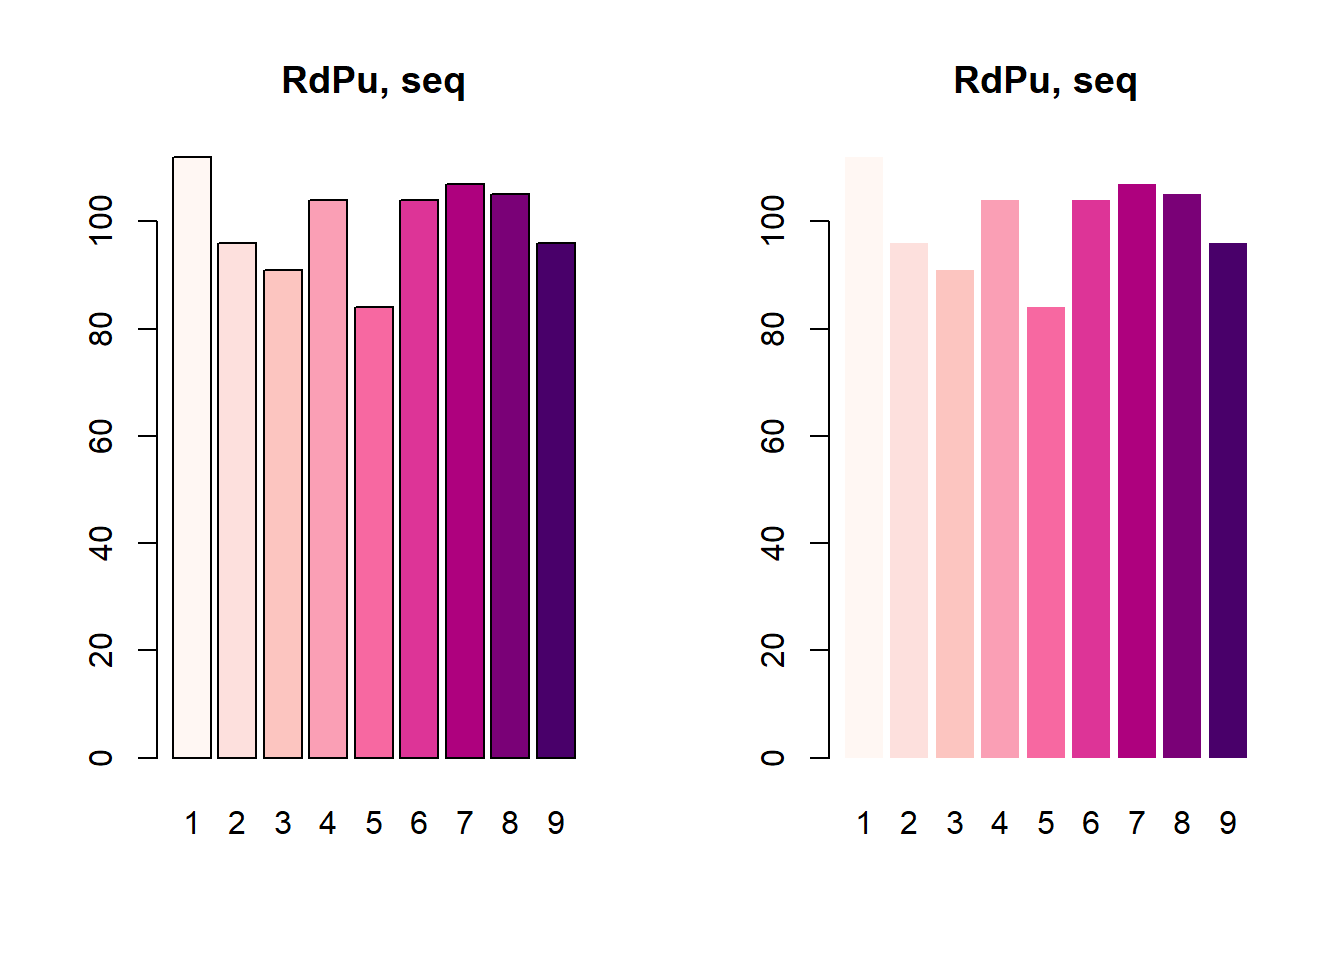
\includegraphics[width=0.9\linewidth]{41-Szinek_files/figure-latex/unnamed-chunk-35-1} \end{center}

\begin{Shaded}
\begin{Highlighting}[]
\FunctionTok{par}\NormalTok{(}\AttributeTok{mfrow =} \FunctionTok{c}\NormalTok{(}\DecValTok{1}\NormalTok{, }\DecValTok{2}\NormalTok{))}
\FunctionTok{barplot}\NormalTok{(x[}\DecValTok{1}\SpecialCharTok{:}\DecValTok{9}\NormalTok{], }\AttributeTok{col =} \FunctionTok{brewer.pal}\NormalTok{(}\AttributeTok{n =} \DecValTok{9}\NormalTok{, }\AttributeTok{name =} \StringTok{"Reds"}\NormalTok{), }\AttributeTok{names.arg =} \DecValTok{1}\SpecialCharTok{:}\DecValTok{9}\NormalTok{, }\AttributeTok{main =} \StringTok{"Reds, seq"}\NormalTok{)}
\FunctionTok{barplot}\NormalTok{(x[}\DecValTok{1}\SpecialCharTok{:}\DecValTok{9}\NormalTok{], }\AttributeTok{col =} \FunctionTok{brewer.pal}\NormalTok{(}\AttributeTok{n =} \DecValTok{9}\NormalTok{, }\AttributeTok{name =} \StringTok{"Reds"}\NormalTok{), }\AttributeTok{names.arg =} \DecValTok{1}\SpecialCharTok{:}\DecValTok{9}\NormalTok{, }\AttributeTok{main =} \StringTok{"Reds, seq"}\NormalTok{, }
    \AttributeTok{border =} \ConstantTok{NA}\NormalTok{)}
\end{Highlighting}
\end{Shaded}

\begin{center}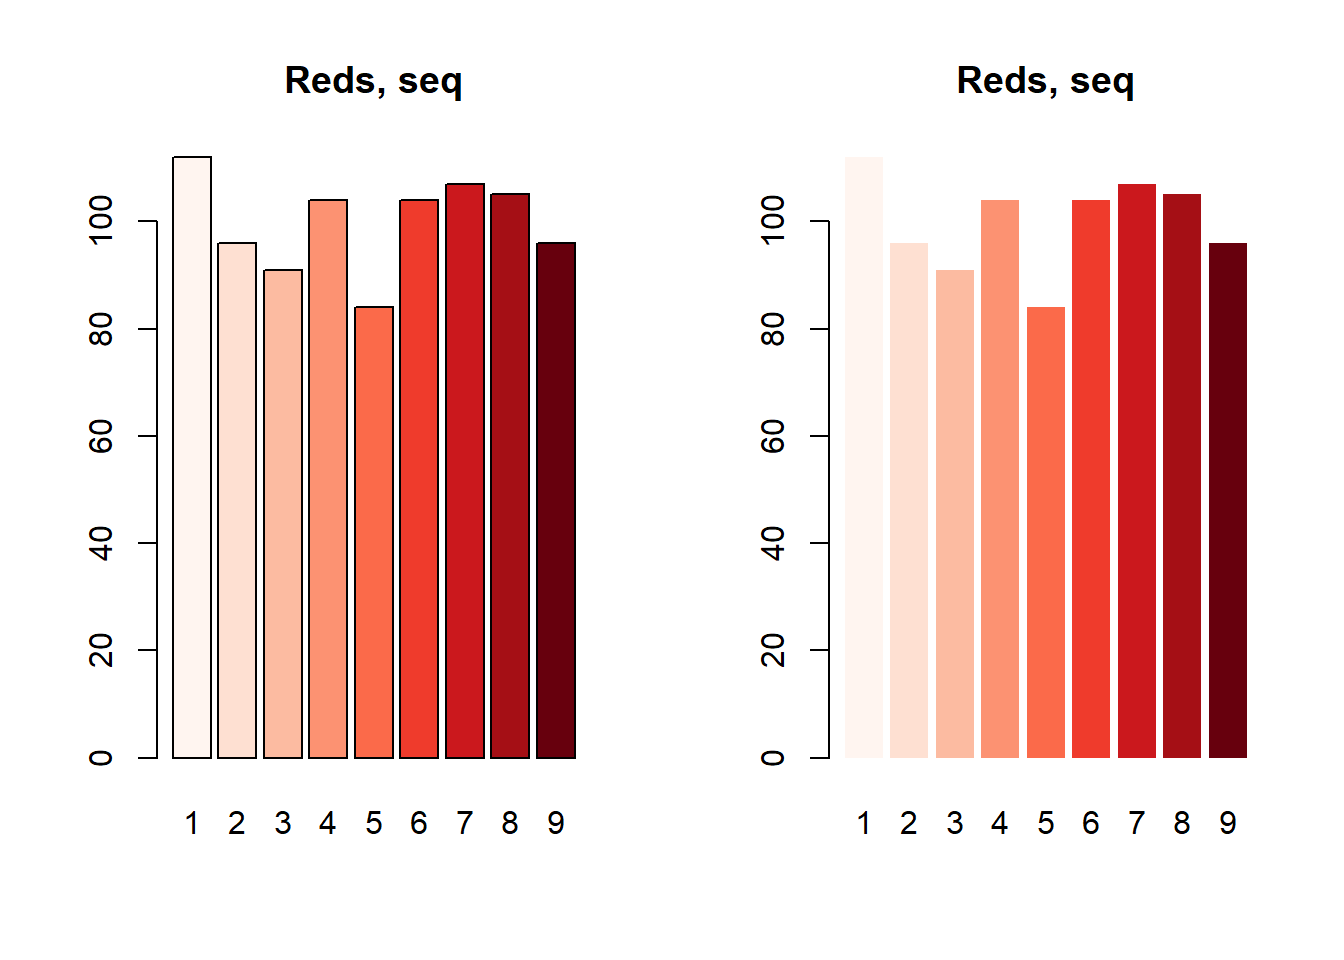
\includegraphics[width=0.9\linewidth]{41-Szinek_files/figure-latex/unnamed-chunk-36-1} \end{center}

\begin{Shaded}
\begin{Highlighting}[]
\FunctionTok{par}\NormalTok{(}\AttributeTok{mfrow =} \FunctionTok{c}\NormalTok{(}\DecValTok{1}\NormalTok{, }\DecValTok{2}\NormalTok{))}
\FunctionTok{barplot}\NormalTok{(x[}\DecValTok{1}\SpecialCharTok{:}\DecValTok{9}\NormalTok{], }\AttributeTok{col =} \FunctionTok{brewer.pal}\NormalTok{(}\AttributeTok{n =} \DecValTok{9}\NormalTok{, }\AttributeTok{name =} \StringTok{"YlGn"}\NormalTok{), }\AttributeTok{names.arg =} \DecValTok{1}\SpecialCharTok{:}\DecValTok{9}\NormalTok{, }\AttributeTok{main =} \StringTok{"YlGn, seq"}\NormalTok{)}
\FunctionTok{barplot}\NormalTok{(x[}\DecValTok{1}\SpecialCharTok{:}\DecValTok{9}\NormalTok{], }\AttributeTok{col =} \FunctionTok{brewer.pal}\NormalTok{(}\AttributeTok{n =} \DecValTok{9}\NormalTok{, }\AttributeTok{name =} \StringTok{"YlGn"}\NormalTok{), }\AttributeTok{names.arg =} \DecValTok{1}\SpecialCharTok{:}\DecValTok{9}\NormalTok{, }\AttributeTok{main =} \StringTok{"YlGn, seq"}\NormalTok{, }
    \AttributeTok{border =} \ConstantTok{NA}\NormalTok{)}
\end{Highlighting}
\end{Shaded}

\begin{center}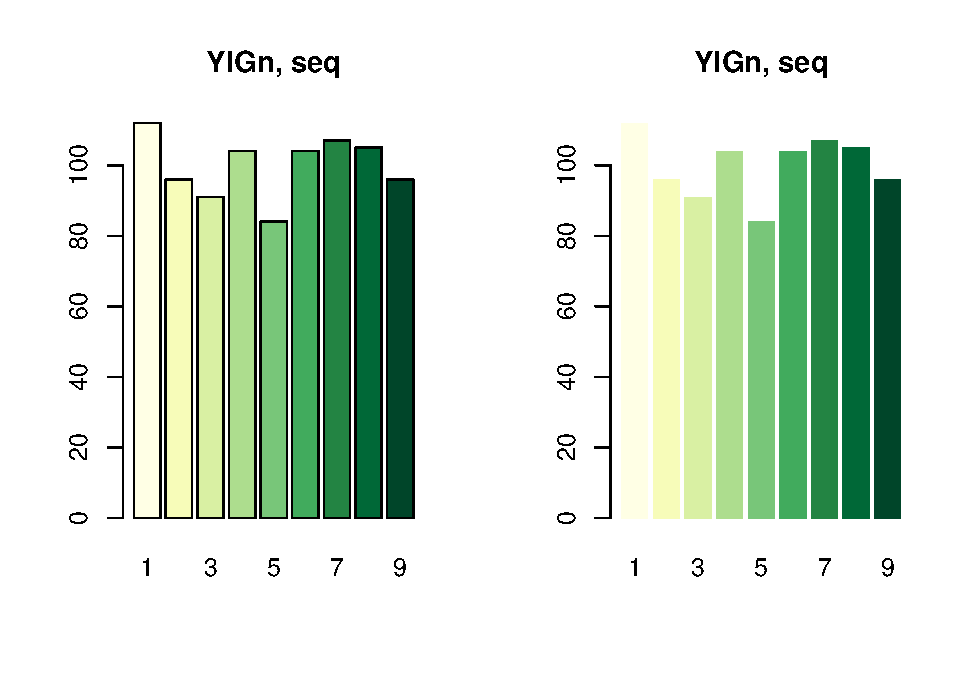
\includegraphics[width=0.9\linewidth]{41-Szinek_files/figure-latex/unnamed-chunk-37-1} \end{center}

\begin{Shaded}
\begin{Highlighting}[]
\FunctionTok{par}\NormalTok{(}\AttributeTok{mfrow =} \FunctionTok{c}\NormalTok{(}\DecValTok{1}\NormalTok{, }\DecValTok{2}\NormalTok{))}
\FunctionTok{barplot}\NormalTok{(x[}\DecValTok{1}\SpecialCharTok{:}\DecValTok{9}\NormalTok{], }\AttributeTok{col =} \FunctionTok{brewer.pal}\NormalTok{(}\AttributeTok{n =} \DecValTok{9}\NormalTok{, }\AttributeTok{name =} \StringTok{"YlGnBu"}\NormalTok{), }\AttributeTok{names.arg =} \DecValTok{1}\SpecialCharTok{:}\DecValTok{9}\NormalTok{, }\AttributeTok{main =} \StringTok{"YlGnBu, seq"}\NormalTok{)}
\FunctionTok{barplot}\NormalTok{(x[}\DecValTok{1}\SpecialCharTok{:}\DecValTok{9}\NormalTok{], }\AttributeTok{col =} \FunctionTok{brewer.pal}\NormalTok{(}\AttributeTok{n =} \DecValTok{9}\NormalTok{, }\AttributeTok{name =} \StringTok{"YlGnBu"}\NormalTok{), }\AttributeTok{names.arg =} \DecValTok{1}\SpecialCharTok{:}\DecValTok{9}\NormalTok{, }\AttributeTok{main =} \StringTok{"YlGnBu, seq"}\NormalTok{, }
    \AttributeTok{border =} \ConstantTok{NA}\NormalTok{)}
\end{Highlighting}
\end{Shaded}

\begin{center}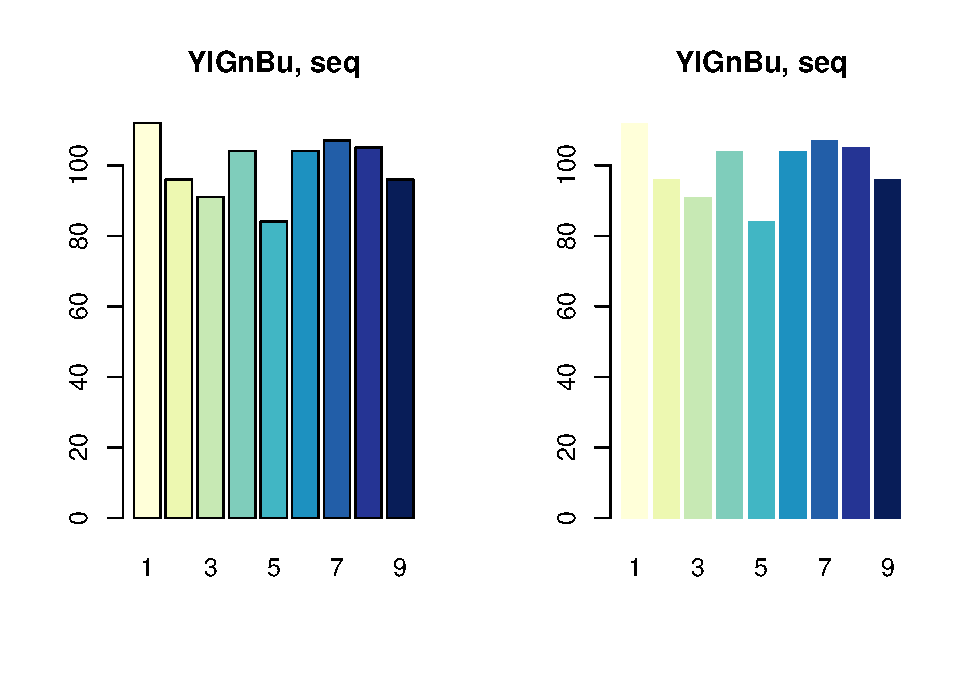
\includegraphics[width=0.9\linewidth]{41-Szinek_files/figure-latex/unnamed-chunk-38-1} \end{center}

\begin{Shaded}
\begin{Highlighting}[]
\FunctionTok{par}\NormalTok{(}\AttributeTok{mfrow =} \FunctionTok{c}\NormalTok{(}\DecValTok{1}\NormalTok{, }\DecValTok{2}\NormalTok{))}
\FunctionTok{barplot}\NormalTok{(x[}\DecValTok{1}\SpecialCharTok{:}\DecValTok{9}\NormalTok{], }\AttributeTok{col =} \FunctionTok{brewer.pal}\NormalTok{(}\AttributeTok{n =} \DecValTok{9}\NormalTok{, }\AttributeTok{name =} \StringTok{"YlOrBr"}\NormalTok{), }\AttributeTok{names.arg =} \DecValTok{1}\SpecialCharTok{:}\DecValTok{9}\NormalTok{, }\AttributeTok{main =} \StringTok{"YlOrBr, seq"}\NormalTok{)}
\FunctionTok{barplot}\NormalTok{(x[}\DecValTok{1}\SpecialCharTok{:}\DecValTok{9}\NormalTok{], }\AttributeTok{col =} \FunctionTok{brewer.pal}\NormalTok{(}\AttributeTok{n =} \DecValTok{9}\NormalTok{, }\AttributeTok{name =} \StringTok{"YlOrBr"}\NormalTok{), }\AttributeTok{names.arg =} \DecValTok{1}\SpecialCharTok{:}\DecValTok{9}\NormalTok{, }\AttributeTok{main =} \StringTok{"YlOrBr, seq"}\NormalTok{, }
    \AttributeTok{border =} \ConstantTok{NA}\NormalTok{)}
\end{Highlighting}
\end{Shaded}

\begin{center}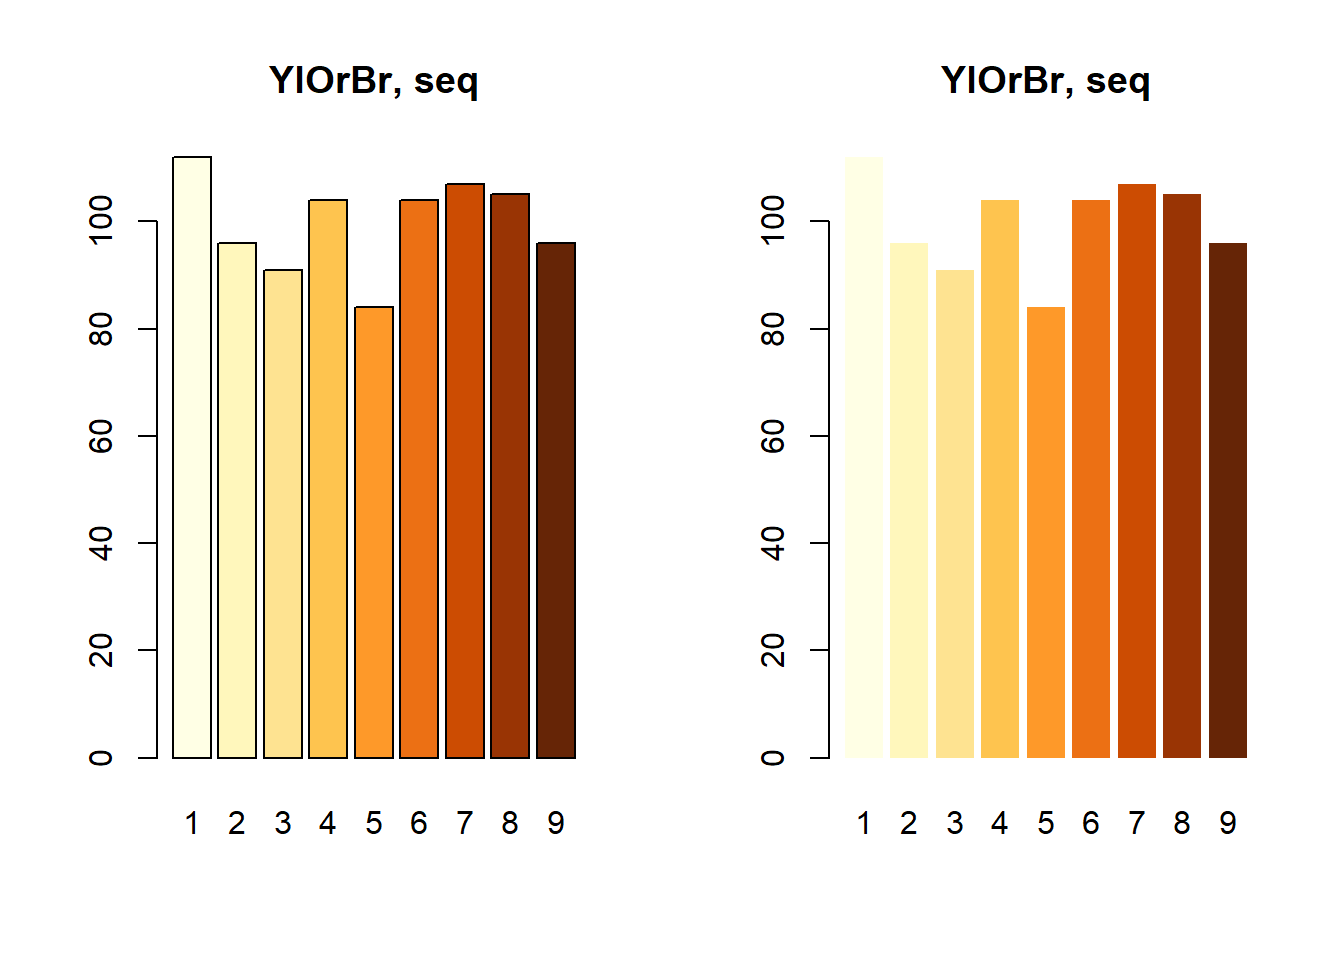
\includegraphics[width=0.9\linewidth]{41-Szinek_files/figure-latex/unnamed-chunk-39-1} \end{center}

\begin{Shaded}
\begin{Highlighting}[]
\FunctionTok{par}\NormalTok{(}\AttributeTok{mfrow =} \FunctionTok{c}\NormalTok{(}\DecValTok{1}\NormalTok{, }\DecValTok{2}\NormalTok{))}
\FunctionTok{barplot}\NormalTok{(x[}\DecValTok{1}\SpecialCharTok{:}\DecValTok{9}\NormalTok{], }\AttributeTok{col =} \FunctionTok{brewer.pal}\NormalTok{(}\AttributeTok{n =} \DecValTok{9}\NormalTok{, }\AttributeTok{name =} \StringTok{"YlOrRd"}\NormalTok{), }\AttributeTok{names.arg =} \DecValTok{1}\SpecialCharTok{:}\DecValTok{9}\NormalTok{, }\AttributeTok{main =} \StringTok{"YlOrRd, seq"}\NormalTok{)}
\FunctionTok{barplot}\NormalTok{(x[}\DecValTok{1}\SpecialCharTok{:}\DecValTok{9}\NormalTok{], }\AttributeTok{col =} \FunctionTok{brewer.pal}\NormalTok{(}\AttributeTok{n =} \DecValTok{9}\NormalTok{, }\AttributeTok{name =} \StringTok{"YlOrRd"}\NormalTok{), }\AttributeTok{names.arg =} \DecValTok{1}\SpecialCharTok{:}\DecValTok{9}\NormalTok{, }\AttributeTok{main =} \StringTok{"YlOrRd, seq"}\NormalTok{, }
    \AttributeTok{border =} \ConstantTok{NA}\NormalTok{)}
\end{Highlighting}
\end{Shaded}

\begin{center}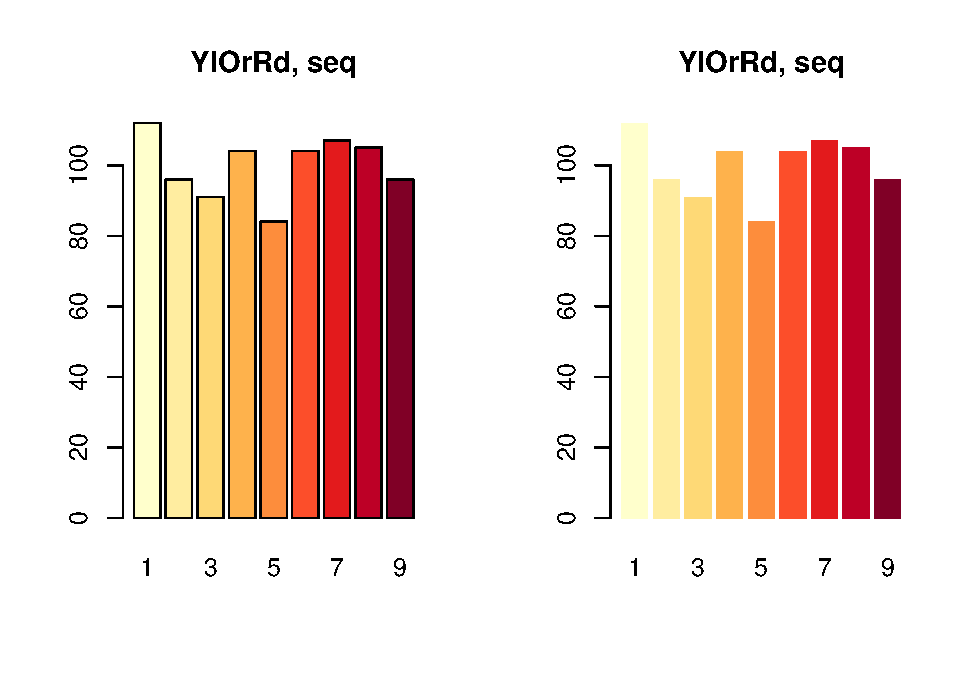
\includegraphics[width=0.9\linewidth]{41-Szinek_files/figure-latex/unnamed-chunk-40-1} \end{center}

\hypertarget{szinek-valasztasa-dichromat}{%
\section{Színek választása a dichromat csomag segítségével}\label{szinek-valasztasa-dichromat}}

A \texttt{dichromat} csomag színsémai közül is választhatunk. A színsémákat a \texttt{colorschemes} lista tartalmazza. A lisatelemek neve:

\begin{Shaded}
\begin{Highlighting}[]
\FunctionTok{library}\NormalTok{(dichromat)}
\FunctionTok{names}\NormalTok{(colorschemes)}
\CommentTok{\#\textgreater{}  [1] "BrowntoBlue.10"         "BrowntoBlue.12"         "BluetoDarkOrange.12"   }
\CommentTok{\#\textgreater{}  [4] "BluetoDarkOrange.18"    "DarkRedtoBlue.12"       "DarkRedtoBlue.18"      }
\CommentTok{\#\textgreater{}  [7] "BluetoGreen.14"         "BluetoGray.8"           "BluetoOrangeRed.14"    }
\CommentTok{\#\textgreater{} [10] "BluetoOrange.10"        "BluetoOrange.12"        "BluetoOrange.8"        }
\CommentTok{\#\textgreater{} [13] "LightBluetoDarkBlue.10" "LightBluetoDarkBlue.7"  "Categorical.12"        }
\CommentTok{\#\textgreater{} [16] "GreentoMagenta.16"      "SteppedSequential.5"}
\end{Highlighting}
\end{Shaded}

Példák színek választására:

\begin{Shaded}
\begin{Highlighting}[]
\CommentTok{\# az x adatvektor beállítása}
\FunctionTok{set.seed}\NormalTok{(}\DecValTok{0}\NormalTok{)}
\NormalTok{x }\OtherTok{\textless{}{-}} \FunctionTok{rpois}\NormalTok{(}\AttributeTok{n =} \DecValTok{50}\NormalTok{, }\AttributeTok{lambda =} \DecValTok{100}\NormalTok{)}
\CommentTok{\# grafikus paraméterek beállítása}
\FunctionTok{par}\NormalTok{(}\AttributeTok{las =} \DecValTok{1}\NormalTok{, }\AttributeTok{mgp =} \FunctionTok{c}\NormalTok{(}\DecValTok{0}\NormalTok{, }\FloatTok{0.2}\NormalTok{, }\DecValTok{0}\NormalTok{), }\AttributeTok{tcl =} \SpecialCharTok{{-}}\FloatTok{0.2}\NormalTok{, }\AttributeTok{mar =} \FunctionTok{c}\NormalTok{(}\DecValTok{3}\NormalTok{, }\DecValTok{2}\NormalTok{, }\DecValTok{1}\NormalTok{, }\DecValTok{1}\NormalTok{))}
\FunctionTok{library}\NormalTok{(dichromat)}
\FunctionTok{par}\NormalTok{(}\AttributeTok{mfrow=}\FunctionTok{c}\NormalTok{(}\DecValTok{1}\NormalTok{,}\DecValTok{2}\NormalTok{))}
\FunctionTok{barplot}\NormalTok{(x[}\DecValTok{1}\SpecialCharTok{:}\DecValTok{10}\NormalTok{], }\AttributeTok{col =}\NormalTok{ colorschemes}\SpecialCharTok{$}\NormalTok{BrowntoBlue}\FloatTok{.10}\NormalTok{, }\AttributeTok{names.arg =} \DecValTok{1}\SpecialCharTok{:}\DecValTok{10}\NormalTok{, }\AttributeTok{main =} \StringTok{"BrowntoBlue.10"}\NormalTok{)}
\FunctionTok{barplot}\NormalTok{(x[}\DecValTok{1}\SpecialCharTok{:}\DecValTok{10}\NormalTok{], }\AttributeTok{col =}\NormalTok{ colorschemes}\SpecialCharTok{$}\NormalTok{BrowntoBlue}\FloatTok{.10}\NormalTok{, }\AttributeTok{names.arg =} \DecValTok{1}\SpecialCharTok{:}\DecValTok{10}\NormalTok{, }\AttributeTok{main =} \StringTok{"BrowntoBlue.10"}\NormalTok{, }\AttributeTok{border=}\ConstantTok{NA}\NormalTok{)}
\end{Highlighting}
\end{Shaded}

\begin{center}\includegraphics[width=0.9\linewidth]{41-Szinek_files/figure-latex/unnamed-chunk-42-1} \end{center}

\begin{Shaded}
\begin{Highlighting}[]
\FunctionTok{par}\NormalTok{(}\AttributeTok{mfrow=}\FunctionTok{c}\NormalTok{(}\DecValTok{1}\NormalTok{,}\DecValTok{2}\NormalTok{))}
\FunctionTok{barplot}\NormalTok{(x[}\DecValTok{1}\SpecialCharTok{:}\DecValTok{12}\NormalTok{], }\AttributeTok{col =}\NormalTok{ colorschemes}\SpecialCharTok{$}\NormalTok{BrowntoBlue}\FloatTok{.12}\NormalTok{, }\AttributeTok{names.arg =} \DecValTok{1}\SpecialCharTok{:}\DecValTok{12}\NormalTok{, }\AttributeTok{main =} \StringTok{"BrowntoBlue.12"}\NormalTok{)}
\FunctionTok{barplot}\NormalTok{(x[}\DecValTok{1}\SpecialCharTok{:}\DecValTok{12}\NormalTok{], }\AttributeTok{col =}\NormalTok{ colorschemes}\SpecialCharTok{$}\NormalTok{BrowntoBlue}\FloatTok{.12}\NormalTok{, }\AttributeTok{names.arg =} \DecValTok{1}\SpecialCharTok{:}\DecValTok{12}\NormalTok{, }\AttributeTok{main =} \StringTok{"BrowntoBlue.12"}\NormalTok{, }\AttributeTok{border =} \ConstantTok{NA}\NormalTok{)}
\end{Highlighting}
\end{Shaded}

\begin{center}\includegraphics[width=0.9\linewidth]{41-Szinek_files/figure-latex/unnamed-chunk-43-1} \end{center}

\begin{Shaded}
\begin{Highlighting}[]
\FunctionTok{par}\NormalTok{(}\AttributeTok{mfrow=}\FunctionTok{c}\NormalTok{(}\DecValTok{1}\NormalTok{,}\DecValTok{2}\NormalTok{))}
\FunctionTok{barplot}\NormalTok{(x[}\DecValTok{1}\SpecialCharTok{:}\DecValTok{12}\NormalTok{], }\AttributeTok{col =}\NormalTok{ colorschemes}\SpecialCharTok{$}\NormalTok{BluetoDarkOrange}\FloatTok{.12}\NormalTok{, }\AttributeTok{names.arg =} \DecValTok{1}\SpecialCharTok{:}\DecValTok{12}\NormalTok{, }\AttributeTok{main =} \StringTok{"BluetoDarkOrange.12"}\NormalTok{)}
\FunctionTok{barplot}\NormalTok{(x[}\DecValTok{1}\SpecialCharTok{:}\DecValTok{12}\NormalTok{], }\AttributeTok{col =}\NormalTok{ colorschemes}\SpecialCharTok{$}\NormalTok{BluetoDarkOrange}\FloatTok{.12}\NormalTok{, }\AttributeTok{names.arg =} \DecValTok{1}\SpecialCharTok{:}\DecValTok{12}\NormalTok{, }\AttributeTok{main =} \StringTok{"BluetoDarkOrange.12"}\NormalTok{, }\AttributeTok{border =} \ConstantTok{NA}\NormalTok{)}
\end{Highlighting}
\end{Shaded}

\begin{center}\includegraphics[width=0.9\linewidth]{41-Szinek_files/figure-latex/unnamed-chunk-44-1} \end{center}

\begin{Shaded}
\begin{Highlighting}[]
\FunctionTok{par}\NormalTok{(}\AttributeTok{mfrow=}\FunctionTok{c}\NormalTok{(}\DecValTok{1}\NormalTok{,}\DecValTok{2}\NormalTok{))}
\FunctionTok{barplot}\NormalTok{(x[}\DecValTok{1}\SpecialCharTok{:}\DecValTok{18}\NormalTok{], }\AttributeTok{col =}\NormalTok{ colorschemes}\SpecialCharTok{$}\NormalTok{BluetoDarkOrange}\FloatTok{.18}\NormalTok{, }\AttributeTok{names.arg =} \DecValTok{1}\SpecialCharTok{:}\DecValTok{18}\NormalTok{, }\AttributeTok{main =} \StringTok{"BluetoDarkOrange.18"}\NormalTok{)}
\FunctionTok{barplot}\NormalTok{(x[}\DecValTok{1}\SpecialCharTok{:}\DecValTok{18}\NormalTok{], }\AttributeTok{col =}\NormalTok{ colorschemes}\SpecialCharTok{$}\NormalTok{BluetoDarkOrange}\FloatTok{.18}\NormalTok{, }\AttributeTok{names.arg =} \DecValTok{1}\SpecialCharTok{:}\DecValTok{18}\NormalTok{, }\AttributeTok{main =} \StringTok{"BluetoDarkOrange.18"}\NormalTok{, }\AttributeTok{border =} \ConstantTok{NA}\NormalTok{)}
\end{Highlighting}
\end{Shaded}

\begin{center}\includegraphics[width=0.9\linewidth]{41-Szinek_files/figure-latex/unnamed-chunk-45-1} \end{center}

\begin{Shaded}
\begin{Highlighting}[]
\FunctionTok{par}\NormalTok{(}\AttributeTok{mfrow=}\FunctionTok{c}\NormalTok{(}\DecValTok{1}\NormalTok{,}\DecValTok{2}\NormalTok{))}
\FunctionTok{barplot}\NormalTok{(x[}\DecValTok{1}\SpecialCharTok{:}\DecValTok{12}\NormalTok{], }\AttributeTok{col =}\NormalTok{ colorschemes}\SpecialCharTok{$}\NormalTok{DarkRedtoBlue}\FloatTok{.12}\NormalTok{, }\AttributeTok{names.arg =} \DecValTok{1}\SpecialCharTok{:}\DecValTok{12}\NormalTok{, }\AttributeTok{main =} \StringTok{"DarkRedtoBlue.12"}\NormalTok{)}
\FunctionTok{barplot}\NormalTok{(x[}\DecValTok{1}\SpecialCharTok{:}\DecValTok{12}\NormalTok{], }\AttributeTok{col =}\NormalTok{ colorschemes}\SpecialCharTok{$}\NormalTok{DarkRedtoBlue}\FloatTok{.12}\NormalTok{, }\AttributeTok{names.arg =} \DecValTok{1}\SpecialCharTok{:}\DecValTok{12}\NormalTok{, }\AttributeTok{main =} \StringTok{"DarkRedtoBlue.12"}\NormalTok{, }\AttributeTok{border =} \ConstantTok{NA}\NormalTok{)}
\end{Highlighting}
\end{Shaded}

\begin{center}\includegraphics[width=0.9\linewidth]{41-Szinek_files/figure-latex/unnamed-chunk-46-1} \end{center}

\begin{Shaded}
\begin{Highlighting}[]
\FunctionTok{par}\NormalTok{(}\AttributeTok{mfrow=}\FunctionTok{c}\NormalTok{(}\DecValTok{1}\NormalTok{,}\DecValTok{2}\NormalTok{))}
\FunctionTok{barplot}\NormalTok{(x[}\DecValTok{1}\SpecialCharTok{:}\DecValTok{18}\NormalTok{], }\AttributeTok{col =}\NormalTok{ colorschemes}\SpecialCharTok{$}\NormalTok{DarkRedtoBlue}\FloatTok{.18}\NormalTok{, }\AttributeTok{names.arg =} \DecValTok{1}\SpecialCharTok{:}\DecValTok{18}\NormalTok{, }\AttributeTok{main =} \StringTok{"DarkRedtoBlue.18"}\NormalTok{)}
\FunctionTok{barplot}\NormalTok{(x[}\DecValTok{1}\SpecialCharTok{:}\DecValTok{18}\NormalTok{], }\AttributeTok{col =}\NormalTok{ colorschemes}\SpecialCharTok{$}\NormalTok{DarkRedtoBlue}\FloatTok{.18}\NormalTok{, }\AttributeTok{names.arg =} \DecValTok{1}\SpecialCharTok{:}\DecValTok{18}\NormalTok{, }\AttributeTok{main =} \StringTok{"DarkRedtoBlue.18"}\NormalTok{, }\AttributeTok{border =} \ConstantTok{NA}\NormalTok{)}
\end{Highlighting}
\end{Shaded}

\begin{center}\includegraphics[width=0.9\linewidth]{41-Szinek_files/figure-latex/unnamed-chunk-47-1} \end{center}

\begin{Shaded}
\begin{Highlighting}[]
\FunctionTok{par}\NormalTok{(}\AttributeTok{mfrow=}\FunctionTok{c}\NormalTok{(}\DecValTok{1}\NormalTok{,}\DecValTok{2}\NormalTok{))}
\FunctionTok{barplot}\NormalTok{(x[}\DecValTok{1}\SpecialCharTok{:}\DecValTok{14}\NormalTok{], }\AttributeTok{col =}\NormalTok{ colorschemes}\SpecialCharTok{$}\NormalTok{BluetoGreen}\FloatTok{.14}\NormalTok{, }\AttributeTok{names.arg =} \DecValTok{1}\SpecialCharTok{:}\DecValTok{14}\NormalTok{, }\AttributeTok{main =} \StringTok{"BluetoGreen.14"}\NormalTok{)}
\FunctionTok{barplot}\NormalTok{(x[}\DecValTok{1}\SpecialCharTok{:}\DecValTok{14}\NormalTok{], }\AttributeTok{col =}\NormalTok{ colorschemes}\SpecialCharTok{$}\NormalTok{BluetoGreen}\FloatTok{.14}\NormalTok{, }\AttributeTok{names.arg =} \DecValTok{1}\SpecialCharTok{:}\DecValTok{14}\NormalTok{, }\AttributeTok{main =} \StringTok{"BluetoGreen.14"}\NormalTok{, }\AttributeTok{border =} \ConstantTok{NA}\NormalTok{)}
\end{Highlighting}
\end{Shaded}

\begin{center}\includegraphics[width=0.9\linewidth]{41-Szinek_files/figure-latex/unnamed-chunk-48-1} \end{center}

\begin{Shaded}
\begin{Highlighting}[]
\FunctionTok{par}\NormalTok{(}\AttributeTok{mfrow=}\FunctionTok{c}\NormalTok{(}\DecValTok{1}\NormalTok{,}\DecValTok{2}\NormalTok{))}
\FunctionTok{barplot}\NormalTok{(x[}\DecValTok{1}\SpecialCharTok{:}\DecValTok{8}\NormalTok{], }\AttributeTok{col =}\NormalTok{ colorschemes}\SpecialCharTok{$}\NormalTok{BluetoGray}\FloatTok{.8}\NormalTok{, }\AttributeTok{names.arg =} \DecValTok{1}\SpecialCharTok{:}\DecValTok{8}\NormalTok{, }\AttributeTok{main =} \StringTok{"BluetoGray.8"}\NormalTok{)}
\FunctionTok{barplot}\NormalTok{(x[}\DecValTok{1}\SpecialCharTok{:}\DecValTok{8}\NormalTok{], }\AttributeTok{col =}\NormalTok{ colorschemes}\SpecialCharTok{$}\NormalTok{BluetoGray}\FloatTok{.8}\NormalTok{, }\AttributeTok{names.arg =} \DecValTok{1}\SpecialCharTok{:}\DecValTok{8}\NormalTok{, }\AttributeTok{main =} \StringTok{"BluetoGray.8"}\NormalTok{, }\AttributeTok{border =} \ConstantTok{NA}\NormalTok{)}
\end{Highlighting}
\end{Shaded}

\begin{center}\includegraphics[width=0.9\linewidth]{41-Szinek_files/figure-latex/unnamed-chunk-49-1} \end{center}

\begin{Shaded}
\begin{Highlighting}[]
\FunctionTok{par}\NormalTok{(}\AttributeTok{mfrow=}\FunctionTok{c}\NormalTok{(}\DecValTok{1}\NormalTok{,}\DecValTok{2}\NormalTok{))}
\FunctionTok{barplot}\NormalTok{(x[}\DecValTok{1}\SpecialCharTok{:}\DecValTok{14}\NormalTok{], }\AttributeTok{col =}\NormalTok{ colorschemes}\SpecialCharTok{$}\NormalTok{BluetoOrangeRed}\FloatTok{.14}\NormalTok{, }\AttributeTok{names.arg =} \DecValTok{1}\SpecialCharTok{:}\DecValTok{14}\NormalTok{, }\AttributeTok{main =} \StringTok{"BluetoOrangeRed.14"}\NormalTok{)}
\FunctionTok{barplot}\NormalTok{(x[}\DecValTok{1}\SpecialCharTok{:}\DecValTok{14}\NormalTok{], }\AttributeTok{col =}\NormalTok{ colorschemes}\SpecialCharTok{$}\NormalTok{BluetoOrangeRed}\FloatTok{.14}\NormalTok{, }\AttributeTok{names.arg =} \DecValTok{1}\SpecialCharTok{:}\DecValTok{14}\NormalTok{, }\AttributeTok{main =} \StringTok{"BluetoOrangeRed.14"}\NormalTok{, }\AttributeTok{border =} \ConstantTok{NA}\NormalTok{)}
\end{Highlighting}
\end{Shaded}

\begin{center}\includegraphics[width=0.9\linewidth]{41-Szinek_files/figure-latex/unnamed-chunk-50-1} \end{center}

\begin{Shaded}
\begin{Highlighting}[]
\FunctionTok{par}\NormalTok{(}\AttributeTok{mfrow=}\FunctionTok{c}\NormalTok{(}\DecValTok{1}\NormalTok{,}\DecValTok{2}\NormalTok{))}
\FunctionTok{barplot}\NormalTok{(x[}\DecValTok{1}\SpecialCharTok{:}\DecValTok{10}\NormalTok{], }\AttributeTok{col =}\NormalTok{ colorschemes}\SpecialCharTok{$}\NormalTok{BluetoOrange}\FloatTok{.10}\NormalTok{, }\AttributeTok{names.arg =} \DecValTok{1}\SpecialCharTok{:}\DecValTok{10}\NormalTok{, }\AttributeTok{main =} \StringTok{"BluetoOrange.10"}\NormalTok{)}
\FunctionTok{barplot}\NormalTok{(x[}\DecValTok{1}\SpecialCharTok{:}\DecValTok{10}\NormalTok{], }\AttributeTok{col =}\NormalTok{ colorschemes}\SpecialCharTok{$}\NormalTok{BluetoOrange}\FloatTok{.10}\NormalTok{, }\AttributeTok{names.arg =} \DecValTok{1}\SpecialCharTok{:}\DecValTok{10}\NormalTok{, }\AttributeTok{main =} \StringTok{"BluetoOrange.10"}\NormalTok{, }\AttributeTok{border =} \ConstantTok{NA}\NormalTok{)}
\end{Highlighting}
\end{Shaded}

\begin{center}\includegraphics[width=0.9\linewidth]{41-Szinek_files/figure-latex/unnamed-chunk-51-1} \end{center}

\begin{Shaded}
\begin{Highlighting}[]
\FunctionTok{par}\NormalTok{(}\AttributeTok{mfrow=}\FunctionTok{c}\NormalTok{(}\DecValTok{1}\NormalTok{,}\DecValTok{2}\NormalTok{))}
\FunctionTok{barplot}\NormalTok{(x[}\DecValTok{1}\SpecialCharTok{:}\DecValTok{12}\NormalTok{], }\AttributeTok{col =}\NormalTok{ colorschemes}\SpecialCharTok{$}\NormalTok{BluetoOrange}\FloatTok{.12}\NormalTok{, }\AttributeTok{names.arg =} \DecValTok{1}\SpecialCharTok{:}\DecValTok{12}\NormalTok{, }\AttributeTok{main =} \StringTok{"BluetoOrange.12"}\NormalTok{)}
\FunctionTok{barplot}\NormalTok{(x[}\DecValTok{1}\SpecialCharTok{:}\DecValTok{12}\NormalTok{], }\AttributeTok{col =}\NormalTok{ colorschemes}\SpecialCharTok{$}\NormalTok{BluetoOrange}\FloatTok{.12}\NormalTok{, }\AttributeTok{names.arg =} \DecValTok{1}\SpecialCharTok{:}\DecValTok{12}\NormalTok{, }\AttributeTok{main =} \StringTok{"BluetoOrange.12"}\NormalTok{, }\AttributeTok{border =}\NormalTok{ T)}
\end{Highlighting}
\end{Shaded}

\begin{center}\includegraphics[width=0.9\linewidth]{41-Szinek_files/figure-latex/unnamed-chunk-52-1} \end{center}

\begin{Shaded}
\begin{Highlighting}[]
\FunctionTok{par}\NormalTok{(}\AttributeTok{mfrow=}\FunctionTok{c}\NormalTok{(}\DecValTok{1}\NormalTok{,}\DecValTok{2}\NormalTok{))}
\FunctionTok{barplot}\NormalTok{(x[}\DecValTok{1}\SpecialCharTok{:}\DecValTok{8}\NormalTok{], }\AttributeTok{col =}\NormalTok{ colorschemes}\SpecialCharTok{$}\NormalTok{BluetoOrange}\FloatTok{.8}\NormalTok{, }\AttributeTok{names.arg =} \DecValTok{1}\SpecialCharTok{:}\DecValTok{8}\NormalTok{, }\AttributeTok{main =} \StringTok{"BluetoOrange.8"}\NormalTok{)}
\FunctionTok{barplot}\NormalTok{(x[}\DecValTok{1}\SpecialCharTok{:}\DecValTok{8}\NormalTok{], }\AttributeTok{col =}\NormalTok{ colorschemes}\SpecialCharTok{$}\NormalTok{BluetoOrange}\FloatTok{.8}\NormalTok{, }\AttributeTok{names.arg =} \DecValTok{1}\SpecialCharTok{:}\DecValTok{8}\NormalTok{, }\AttributeTok{main =} \StringTok{"BluetoOrange.8"}\NormalTok{, }\AttributeTok{border =} \ConstantTok{NA}\NormalTok{)}
\end{Highlighting}
\end{Shaded}

\begin{center}\includegraphics[width=0.9\linewidth]{41-Szinek_files/figure-latex/unnamed-chunk-53-1} \end{center}

\begin{Shaded}
\begin{Highlighting}[]
\FunctionTok{par}\NormalTok{(}\AttributeTok{mfrow=}\FunctionTok{c}\NormalTok{(}\DecValTok{1}\NormalTok{,}\DecValTok{2}\NormalTok{))}
\FunctionTok{barplot}\NormalTok{(x[}\DecValTok{1}\SpecialCharTok{:}\DecValTok{10}\NormalTok{], }\AttributeTok{col =}\NormalTok{ colorschemes}\SpecialCharTok{$}\NormalTok{LightBluetoDarkBlue}\FloatTok{.10}\NormalTok{, }\AttributeTok{names.arg =} \DecValTok{1}\SpecialCharTok{:}\DecValTok{10}\NormalTok{, }
    \AttributeTok{main =} \StringTok{"LightBluetoDarkBlue.10"}\NormalTok{)}
\FunctionTok{barplot}\NormalTok{(x[}\DecValTok{1}\SpecialCharTok{:}\DecValTok{10}\NormalTok{], }\AttributeTok{col =}\NormalTok{ colorschemes}\SpecialCharTok{$}\NormalTok{LightBluetoDarkBlue}\FloatTok{.10}\NormalTok{, }\AttributeTok{names.arg =} \DecValTok{1}\SpecialCharTok{:}\DecValTok{10}\NormalTok{, }
    \AttributeTok{main =} \StringTok{"LightBluetoDarkBlue.10"}\NormalTok{, }\AttributeTok{border =} \ConstantTok{NA}\NormalTok{)}
\end{Highlighting}
\end{Shaded}

\begin{center}\includegraphics[width=0.9\linewidth]{41-Szinek_files/figure-latex/unnamed-chunk-54-1} \end{center}

\begin{Shaded}
\begin{Highlighting}[]
\FunctionTok{par}\NormalTok{(}\AttributeTok{mfrow=}\FunctionTok{c}\NormalTok{(}\DecValTok{1}\NormalTok{,}\DecValTok{2}\NormalTok{))}
\FunctionTok{barplot}\NormalTok{(x[}\DecValTok{1}\SpecialCharTok{:}\DecValTok{7}\NormalTok{], }\AttributeTok{col =}\NormalTok{ colorschemes}\SpecialCharTok{$}\NormalTok{LightBluetoDarkBlue}\FloatTok{.7}\NormalTok{, }\AttributeTok{names.arg =} \DecValTok{1}\SpecialCharTok{:}\DecValTok{7}\NormalTok{, }\AttributeTok{main =} \StringTok{"LightBluetoDarkBlue.7"}\NormalTok{)}
\FunctionTok{barplot}\NormalTok{(x[}\DecValTok{1}\SpecialCharTok{:}\DecValTok{7}\NormalTok{], }\AttributeTok{col =}\NormalTok{ colorschemes}\SpecialCharTok{$}\NormalTok{LightBluetoDarkBlue}\FloatTok{.7}\NormalTok{, }\AttributeTok{names.arg =} \DecValTok{1}\SpecialCharTok{:}\DecValTok{7}\NormalTok{, }\AttributeTok{main =} \StringTok{"LightBluetoDarkBlue.7"}\NormalTok{, }\AttributeTok{border =} \ConstantTok{NA}\NormalTok{)}
\end{Highlighting}
\end{Shaded}

\begin{center}\includegraphics[width=0.9\linewidth]{41-Szinek_files/figure-latex/unnamed-chunk-55-1} \end{center}

\begin{Shaded}
\begin{Highlighting}[]
\FunctionTok{par}\NormalTok{(}\AttributeTok{mfrow=}\FunctionTok{c}\NormalTok{(}\DecValTok{1}\NormalTok{,}\DecValTok{2}\NormalTok{))}
\FunctionTok{barplot}\NormalTok{(x[}\DecValTok{1}\SpecialCharTok{:}\DecValTok{12}\NormalTok{], }\AttributeTok{col =}\NormalTok{ colorschemes}\SpecialCharTok{$}\NormalTok{Categorical}\FloatTok{.12}\NormalTok{, }\AttributeTok{names.arg =} \DecValTok{1}\SpecialCharTok{:}\DecValTok{12}\NormalTok{, }\AttributeTok{main =} \StringTok{"Categorical.12"}\NormalTok{)}
\FunctionTok{barplot}\NormalTok{(x[}\DecValTok{1}\SpecialCharTok{:}\DecValTok{12}\NormalTok{], }\AttributeTok{col =}\NormalTok{ colorschemes}\SpecialCharTok{$}\NormalTok{Categorical}\FloatTok{.12}\NormalTok{, }\AttributeTok{names.arg =} \DecValTok{1}\SpecialCharTok{:}\DecValTok{12}\NormalTok{, }\AttributeTok{main =} \StringTok{"Categorical.12"}\NormalTok{, }\AttributeTok{border =} \ConstantTok{NA}\NormalTok{)}
\end{Highlighting}
\end{Shaded}

\begin{center}\includegraphics[width=0.9\linewidth]{41-Szinek_files/figure-latex/unnamed-chunk-56-1} \end{center}

\begin{Shaded}
\begin{Highlighting}[]
\FunctionTok{par}\NormalTok{(}\AttributeTok{mfrow=}\FunctionTok{c}\NormalTok{(}\DecValTok{1}\NormalTok{,}\DecValTok{2}\NormalTok{))}
\FunctionTok{barplot}\NormalTok{(x[}\DecValTok{1}\SpecialCharTok{:}\DecValTok{16}\NormalTok{], }\AttributeTok{col =}\NormalTok{ colorschemes}\SpecialCharTok{$}\NormalTok{GreentoMagenta}\FloatTok{.16}\NormalTok{, }\AttributeTok{names.arg =} \DecValTok{1}\SpecialCharTok{:}\DecValTok{16}\NormalTok{, }\AttributeTok{main =} \StringTok{"GreentoMagenta.16"}\NormalTok{)}
\FunctionTok{barplot}\NormalTok{(x[}\DecValTok{1}\SpecialCharTok{:}\DecValTok{16}\NormalTok{], }\AttributeTok{col =}\NormalTok{ colorschemes}\SpecialCharTok{$}\NormalTok{GreentoMagenta}\FloatTok{.16}\NormalTok{, }\AttributeTok{names.arg =} \DecValTok{1}\SpecialCharTok{:}\DecValTok{16}\NormalTok{, }\AttributeTok{main =} \StringTok{"GreentoMagenta.16"}\NormalTok{, }\AttributeTok{border =} \ConstantTok{NA}\NormalTok{)}
\end{Highlighting}
\end{Shaded}

\begin{center}\includegraphics[width=0.9\linewidth]{41-Szinek_files/figure-latex/unnamed-chunk-57-1} \end{center}

\begin{Shaded}
\begin{Highlighting}[]
\FunctionTok{par}\NormalTok{(}\AttributeTok{mfrow=}\FunctionTok{c}\NormalTok{(}\DecValTok{1}\NormalTok{,}\DecValTok{2}\NormalTok{))}
\FunctionTok{barplot}\NormalTok{(x[}\DecValTok{1}\SpecialCharTok{:}\DecValTok{25}\NormalTok{], }\AttributeTok{col =}\NormalTok{ colorschemes}\SpecialCharTok{$}\NormalTok{SteppedSequential}\FloatTok{.5}\NormalTok{, }\AttributeTok{names.arg =} \DecValTok{1}\SpecialCharTok{:}\DecValTok{25}\NormalTok{, }\AttributeTok{main =} \StringTok{"SteppedSequential.5"}\NormalTok{)}
\FunctionTok{barplot}\NormalTok{(x[}\DecValTok{1}\SpecialCharTok{:}\DecValTok{25}\NormalTok{], }\AttributeTok{col =}\NormalTok{ colorschemes}\SpecialCharTok{$}\NormalTok{SteppedSequential}\FloatTok{.5}\NormalTok{, }\AttributeTok{names.arg =} \DecValTok{1}\SpecialCharTok{:}\DecValTok{25}\NormalTok{, }\AttributeTok{main =} \StringTok{"SteppedSequential.5"}\NormalTok{, }\AttributeTok{border =} \ConstantTok{NA}\NormalTok{)}
\end{Highlighting}
\end{Shaded}

\begin{center}\includegraphics[width=0.9\linewidth]{41-Szinek_files/figure-latex/unnamed-chunk-58-1} \end{center}

\hypertarget{szinek-valasztasa-egyeb}{%
\section{Színek választása egyéb paletta segítségével}\label{szinek-valasztasa-egyeb}}

Színpaletta létrehozásához több beépített lehetőségek közül is választhatunk.

\begin{Shaded}
\begin{Highlighting}[]
\FunctionTok{rainbow}\NormalTok{(n, }\AttributeTok{start=}\DecValTok{0}\NormalTok{, end, }\AttributeTok{alpha =} \DecValTok{1}\NormalTok{)}
\FunctionTok{heat.colors}\NormalTok{(n, }\AttributeTok{alpha =} \DecValTok{1}\NormalTok{)}
\FunctionTok{terrain.colors}\NormalTok{(n, }\AttributeTok{alpha =} \DecValTok{1}\NormalTok{)}
\FunctionTok{topo.colors}\NormalTok{(n, }\AttributeTok{alpha =} \DecValTok{1}\NormalTok{)}
\FunctionTok{cm.colors}\NormalTok{(n, }\AttributeTok{alpha =} \DecValTok{1}\NormalTok{)}
\end{Highlighting}
\end{Shaded}

Az \texttt{n=} argumentum a létrehozandó színek számát jelenti.

Példák színpaletta létrehozására:

\begin{Shaded}
\begin{Highlighting}[]
\CommentTok{\# az x adatvektor beállítása}
\FunctionTok{set.seed}\NormalTok{(}\DecValTok{0}\NormalTok{)}
\NormalTok{x }\OtherTok{\textless{}{-}} \FunctionTok{rpois}\NormalTok{(}\AttributeTok{n =} \DecValTok{50}\NormalTok{, }\AttributeTok{lambda =} \DecValTok{100}\NormalTok{)}
\CommentTok{\# grafikus paraméterek beállítása}
\FunctionTok{par}\NormalTok{(}\AttributeTok{las =} \DecValTok{1}\NormalTok{, }\AttributeTok{mgp =} \FunctionTok{c}\NormalTok{(}\DecValTok{0}\NormalTok{, }\FloatTok{0.2}\NormalTok{, }\DecValTok{0}\NormalTok{), }\AttributeTok{tcl =} \SpecialCharTok{{-}}\FloatTok{0.2}\NormalTok{, }\AttributeTok{mar =} \FunctionTok{c}\NormalTok{(}\DecValTok{3}\NormalTok{, }\DecValTok{2}\NormalTok{, }\DecValTok{1}\NormalTok{, }\DecValTok{1}\NormalTok{))}
\FunctionTok{par}\NormalTok{(}\AttributeTok{mfrow=}\FunctionTok{c}\NormalTok{(}\DecValTok{1}\NormalTok{,}\DecValTok{2}\NormalTok{))}
\FunctionTok{barplot}\NormalTok{(x[}\DecValTok{1}\SpecialCharTok{:}\DecValTok{16}\NormalTok{], }\AttributeTok{col =} \FunctionTok{rainbow}\NormalTok{(}\DecValTok{16}\NormalTok{), }\AttributeTok{names.arg =} \DecValTok{1}\SpecialCharTok{:}\DecValTok{16}\NormalTok{, }\AttributeTok{main =} \StringTok{"rainbow(n=16)"}\NormalTok{)}
\FunctionTok{barplot}\NormalTok{(x[}\DecValTok{1}\SpecialCharTok{:}\DecValTok{16}\NormalTok{], }\AttributeTok{col =} \FunctionTok{rainbow}\NormalTok{(}\DecValTok{16}\NormalTok{), }\AttributeTok{names.arg =} \DecValTok{1}\SpecialCharTok{:}\DecValTok{16}\NormalTok{, }\AttributeTok{main =} \StringTok{"rainbow(n=16)"}\NormalTok{, }\AttributeTok{border =} \ConstantTok{NA}\NormalTok{)}
\end{Highlighting}
\end{Shaded}

\begin{center}\includegraphics[width=0.9\linewidth]{41-Szinek_files/figure-latex/unnamed-chunk-60-1} \end{center}

\begin{Shaded}
\begin{Highlighting}[]
\FunctionTok{par}\NormalTok{(}\AttributeTok{mfrow=}\FunctionTok{c}\NormalTok{(}\DecValTok{1}\NormalTok{,}\DecValTok{2}\NormalTok{))}
\FunctionTok{barplot}\NormalTok{(x[}\DecValTok{1}\SpecialCharTok{:}\DecValTok{16}\NormalTok{], }\AttributeTok{col =} \FunctionTok{rainbow}\NormalTok{(}\DecValTok{16}\NormalTok{, }\AttributeTok{start =} \DecValTok{0}\NormalTok{, }\AttributeTok{end =} \FloatTok{0.2}\NormalTok{), }\AttributeTok{names.arg =} \DecValTok{1}\SpecialCharTok{:}\DecValTok{16}\NormalTok{, }
    \AttributeTok{main =} \StringTok{"rainbow(n=16, start=0, end=0.2)"}\NormalTok{)}
\FunctionTok{barplot}\NormalTok{(x[}\DecValTok{1}\SpecialCharTok{:}\DecValTok{16}\NormalTok{], }\AttributeTok{col =} \FunctionTok{rainbow}\NormalTok{(}\DecValTok{16}\NormalTok{, }\AttributeTok{start =} \DecValTok{0}\NormalTok{, }\AttributeTok{end =} \FloatTok{0.2}\NormalTok{), }\AttributeTok{names.arg =} \DecValTok{1}\SpecialCharTok{:}\DecValTok{16}\NormalTok{, }
    \AttributeTok{main =} \StringTok{"rainbow(n=16, start=0, end=0.2)"}\NormalTok{, }\AttributeTok{border =} \ConstantTok{NA}\NormalTok{)}
\end{Highlighting}
\end{Shaded}

\begin{center}\includegraphics[width=0.9\linewidth]{41-Szinek_files/figure-latex/unnamed-chunk-61-1} \end{center}

\begin{Shaded}
\begin{Highlighting}[]
\FunctionTok{par}\NormalTok{(}\AttributeTok{mfrow=}\FunctionTok{c}\NormalTok{(}\DecValTok{1}\NormalTok{,}\DecValTok{2}\NormalTok{))}
\FunctionTok{barplot}\NormalTok{(x[}\DecValTok{1}\SpecialCharTok{:}\DecValTok{16}\NormalTok{], }\AttributeTok{col =} \FunctionTok{rainbow}\NormalTok{(}\DecValTok{16}\NormalTok{, }\AttributeTok{start =} \DecValTok{0}\NormalTok{, }\AttributeTok{end =} \FloatTok{0.5}\NormalTok{), }\AttributeTok{names.arg =} \DecValTok{1}\SpecialCharTok{:}\DecValTok{16}\NormalTok{, }
    \AttributeTok{main =} \StringTok{"rainbow(n=16, start=0, end=0.5)"}\NormalTok{)}
\FunctionTok{barplot}\NormalTok{(x[}\DecValTok{1}\SpecialCharTok{:}\DecValTok{16}\NormalTok{], }\AttributeTok{col =} \FunctionTok{rainbow}\NormalTok{(}\DecValTok{16}\NormalTok{, }\AttributeTok{start =} \DecValTok{0}\NormalTok{, }\AttributeTok{end =} \FloatTok{0.5}\NormalTok{), }\AttributeTok{names.arg =} \DecValTok{1}\SpecialCharTok{:}\DecValTok{16}\NormalTok{, }
    \AttributeTok{main =} \StringTok{"rainbow(n=16, start=0, end=0.5)"}\NormalTok{, }\AttributeTok{border =} \ConstantTok{NA}\NormalTok{)}
\end{Highlighting}
\end{Shaded}

\begin{center}\includegraphics[width=0.9\linewidth]{41-Szinek_files/figure-latex/unnamed-chunk-62-1} \end{center}

\begin{Shaded}
\begin{Highlighting}[]
\FunctionTok{par}\NormalTok{(}\AttributeTok{mfrow=}\FunctionTok{c}\NormalTok{(}\DecValTok{1}\NormalTok{,}\DecValTok{2}\NormalTok{))}
\FunctionTok{barplot}\NormalTok{(x[}\DecValTok{1}\SpecialCharTok{:}\DecValTok{16}\NormalTok{], }\AttributeTok{col =} \FunctionTok{rainbow}\NormalTok{(}\DecValTok{16}\NormalTok{, }\AttributeTok{start =} \DecValTok{0}\NormalTok{, }\AttributeTok{end =} \FloatTok{0.8}\NormalTok{), }\AttributeTok{names.arg =} \DecValTok{1}\SpecialCharTok{:}\DecValTok{16}\NormalTok{, }
    \AttributeTok{main =} \StringTok{"rainbow(n=16, start=0, end=0.8)"}\NormalTok{)}
\FunctionTok{barplot}\NormalTok{(x[}\DecValTok{1}\SpecialCharTok{:}\DecValTok{16}\NormalTok{], }\AttributeTok{col =} \FunctionTok{rainbow}\NormalTok{(}\DecValTok{16}\NormalTok{, }\AttributeTok{start =} \DecValTok{0}\NormalTok{, }\AttributeTok{end =} \FloatTok{0.8}\NormalTok{), }\AttributeTok{names.arg =} \DecValTok{1}\SpecialCharTok{:}\DecValTok{16}\NormalTok{, }
    \AttributeTok{main =} \StringTok{"rainbow(n=16, start=0, end=0.8)"}\NormalTok{, }\AttributeTok{border =} \ConstantTok{NA}\NormalTok{)}
\end{Highlighting}
\end{Shaded}

\begin{center}\includegraphics[width=0.9\linewidth]{41-Szinek_files/figure-latex/unnamed-chunk-63-1} \end{center}

\begin{Shaded}
\begin{Highlighting}[]
\FunctionTok{par}\NormalTok{(}\AttributeTok{mfrow=}\FunctionTok{c}\NormalTok{(}\DecValTok{1}\NormalTok{,}\DecValTok{2}\NormalTok{))}
\FunctionTok{barplot}\NormalTok{(x[}\DecValTok{1}\SpecialCharTok{:}\DecValTok{16}\NormalTok{], }\AttributeTok{col =} \FunctionTok{heat.colors}\NormalTok{(}\DecValTok{16}\NormalTok{), }\AttributeTok{names.arg =} \DecValTok{1}\SpecialCharTok{:}\DecValTok{16}\NormalTok{, }\AttributeTok{main =} \StringTok{"heat.colors(n=16)"}\NormalTok{)}
\FunctionTok{barplot}\NormalTok{(x[}\DecValTok{1}\SpecialCharTok{:}\DecValTok{16}\NormalTok{], }\AttributeTok{col =} \FunctionTok{heat.colors}\NormalTok{(}\DecValTok{16}\NormalTok{), }\AttributeTok{names.arg =} \DecValTok{1}\SpecialCharTok{:}\DecValTok{16}\NormalTok{, }\AttributeTok{main =} \StringTok{"heat.colors(n=16)"}\NormalTok{, }\AttributeTok{border =} \ConstantTok{NA}\NormalTok{)}
\end{Highlighting}
\end{Shaded}

\begin{center}\includegraphics[width=0.9\linewidth]{41-Szinek_files/figure-latex/unnamed-chunk-64-1} \end{center}

\begin{Shaded}
\begin{Highlighting}[]
\FunctionTok{par}\NormalTok{(}\AttributeTok{mfrow=}\FunctionTok{c}\NormalTok{(}\DecValTok{1}\NormalTok{,}\DecValTok{2}\NormalTok{))}
\FunctionTok{barplot}\NormalTok{(x[}\DecValTok{1}\SpecialCharTok{:}\DecValTok{16}\NormalTok{], }\AttributeTok{col =} \FunctionTok{terrain.colors}\NormalTok{(}\DecValTok{16}\NormalTok{), }\AttributeTok{names.arg =} \DecValTok{1}\SpecialCharTok{:}\DecValTok{16}\NormalTok{, }\AttributeTok{main =} \StringTok{"terrain.colors(n=16)"}\NormalTok{)}
\FunctionTok{barplot}\NormalTok{(x[}\DecValTok{1}\SpecialCharTok{:}\DecValTok{16}\NormalTok{], }\AttributeTok{col =} \FunctionTok{terrain.colors}\NormalTok{(}\DecValTok{16}\NormalTok{), }\AttributeTok{names.arg =} \DecValTok{1}\SpecialCharTok{:}\DecValTok{16}\NormalTok{, }\AttributeTok{main =} \StringTok{"terrain.colors(n=16)"}\NormalTok{, }\AttributeTok{border =} \ConstantTok{NA}\NormalTok{)}
\end{Highlighting}
\end{Shaded}

\begin{center}\includegraphics[width=0.9\linewidth]{41-Szinek_files/figure-latex/unnamed-chunk-65-1} \end{center}

\begin{Shaded}
\begin{Highlighting}[]
\FunctionTok{par}\NormalTok{(}\AttributeTok{mfrow=}\FunctionTok{c}\NormalTok{(}\DecValTok{1}\NormalTok{,}\DecValTok{2}\NormalTok{))}
\FunctionTok{barplot}\NormalTok{(x[}\DecValTok{1}\SpecialCharTok{:}\DecValTok{16}\NormalTok{], }\AttributeTok{col =} \FunctionTok{topo.colors}\NormalTok{(}\DecValTok{16}\NormalTok{), }\AttributeTok{names.arg =} \DecValTok{1}\SpecialCharTok{:}\DecValTok{16}\NormalTok{, }\AttributeTok{main =} \StringTok{"topo.colors(n=16)"}\NormalTok{)}
\FunctionTok{barplot}\NormalTok{(x[}\DecValTok{1}\SpecialCharTok{:}\DecValTok{16}\NormalTok{], }\AttributeTok{col =} \FunctionTok{topo.colors}\NormalTok{(}\DecValTok{16}\NormalTok{), }\AttributeTok{names.arg =} \DecValTok{1}\SpecialCharTok{:}\DecValTok{16}\NormalTok{, }\AttributeTok{main =} \StringTok{"topo.colors(n=16)"}\NormalTok{, }\AttributeTok{border =} \ConstantTok{NA}\NormalTok{)}
\end{Highlighting}
\end{Shaded}

\begin{center}\includegraphics[width=0.9\linewidth]{41-Szinek_files/figure-latex/unnamed-chunk-66-1} \end{center}

\begin{Shaded}
\begin{Highlighting}[]
\FunctionTok{par}\NormalTok{(}\AttributeTok{mfrow=}\FunctionTok{c}\NormalTok{(}\DecValTok{1}\NormalTok{,}\DecValTok{2}\NormalTok{))}
\FunctionTok{barplot}\NormalTok{(x[}\DecValTok{1}\SpecialCharTok{:}\DecValTok{16}\NormalTok{], }\AttributeTok{col =} \FunctionTok{cm.colors}\NormalTok{(}\DecValTok{16}\NormalTok{), }\AttributeTok{names.arg =} \DecValTok{1}\SpecialCharTok{:}\DecValTok{16}\NormalTok{, }\AttributeTok{main =} \StringTok{"cm.colors(n=16)"}\NormalTok{)}
\FunctionTok{barplot}\NormalTok{(x[}\DecValTok{1}\SpecialCharTok{:}\DecValTok{16}\NormalTok{], }\AttributeTok{col =} \FunctionTok{cm.colors}\NormalTok{(}\DecValTok{16}\NormalTok{), }\AttributeTok{names.arg =} \DecValTok{1}\SpecialCharTok{:}\DecValTok{16}\NormalTok{, }\AttributeTok{main =} \StringTok{"cm.colors(n=16)"}\NormalTok{, }\AttributeTok{border =} \ConstantTok{NA}\NormalTok{)}
\end{Highlighting}
\end{Shaded}

\begin{center}\includegraphics[width=0.9\linewidth]{41-Szinek_files/figure-latex/unnamed-chunk-67-1} \end{center}

\hypertarget{a-657-szinnev}{%
\section{A 657 színnév}\label{a-657-szinnev}}

\begin{Shaded}
\begin{Highlighting}[]
\FunctionTok{colors}\NormalTok{()}
\CommentTok{\#\textgreater{}   [1] "white"                "aliceblue"            "antiquewhite"        }
\CommentTok{\#\textgreater{}   [4] "antiquewhite1"        "antiquewhite2"        "antiquewhite3"       }
\CommentTok{\#\textgreater{}   [7] "antiquewhite4"        "aquamarine"           "aquamarine1"         }
\CommentTok{\#\textgreater{}  [10] "aquamarine2"          "aquamarine3"          "aquamarine4"         }
\CommentTok{\#\textgreater{}  [13] "azure"                "azure1"               "azure2"              }
\CommentTok{\#\textgreater{}  [16] "azure3"               "azure4"               "beige"               }
\CommentTok{\#\textgreater{}  [19] "bisque"               "bisque1"              "bisque2"             }
\CommentTok{\#\textgreater{}  [22] "bisque3"              "bisque4"              "black"               }
\CommentTok{\#\textgreater{}  [25] "blanchedalmond"       "blue"                 "blue1"               }
\CommentTok{\#\textgreater{}  [28] "blue2"                "blue3"                "blue4"               }
\CommentTok{\#\textgreater{}  [31] "blueviolet"           "brown"                "brown1"              }
\CommentTok{\#\textgreater{}  [34] "brown2"               "brown3"               "brown4"              }
\CommentTok{\#\textgreater{}  [37] "burlywood"            "burlywood1"           "burlywood2"          }
\CommentTok{\#\textgreater{}  [40] "burlywood3"           "burlywood4"           "cadetblue"           }
\CommentTok{\#\textgreater{}  [43] "cadetblue1"           "cadetblue2"           "cadetblue3"          }
\CommentTok{\#\textgreater{}  [46] "cadetblue4"           "chartreuse"           "chartreuse1"         }
\CommentTok{\#\textgreater{}  [49] "chartreuse2"          "chartreuse3"          "chartreuse4"         }
\CommentTok{\#\textgreater{}  [52] "chocolate"            "chocolate1"           "chocolate2"          }
\CommentTok{\#\textgreater{}  [55] "chocolate3"           "chocolate4"           "coral"               }
\CommentTok{\#\textgreater{}  [58] "coral1"               "coral2"               "coral3"              }
\CommentTok{\#\textgreater{}  [61] "coral4"               "cornflowerblue"       "cornsilk"            }
\CommentTok{\#\textgreater{}  [64] "cornsilk1"            "cornsilk2"            "cornsilk3"           }
\CommentTok{\#\textgreater{}  [67] "cornsilk4"            "cyan"                 "cyan1"               }
\CommentTok{\#\textgreater{}  [70] "cyan2"                "cyan3"                "cyan4"               }
\CommentTok{\#\textgreater{}  [73] "darkblue"             "darkcyan"             "darkgoldenrod"       }
\CommentTok{\#\textgreater{}  [76] "darkgoldenrod1"       "darkgoldenrod2"       "darkgoldenrod3"      }
\CommentTok{\#\textgreater{}  [79] "darkgoldenrod4"       "darkgray"             "darkgreen"           }
\CommentTok{\#\textgreater{}  [82] "darkgrey"             "darkkhaki"            "darkmagenta"         }
\CommentTok{\#\textgreater{}  [85] "darkolivegreen"       "darkolivegreen1"      "darkolivegreen2"     }
\CommentTok{\#\textgreater{}  [88] "darkolivegreen3"      "darkolivegreen4"      "darkorange"          }
\CommentTok{\#\textgreater{}  [91] "darkorange1"          "darkorange2"          "darkorange3"         }
\CommentTok{\#\textgreater{}  [94] "darkorange4"          "darkorchid"           "darkorchid1"         }
\CommentTok{\#\textgreater{}  [97] "darkorchid2"          "darkorchid3"          "darkorchid4"         }
\CommentTok{\#\textgreater{} [100] "darkred"              "darksalmon"           "darkseagreen"        }
\CommentTok{\#\textgreater{} [103] "darkseagreen1"        "darkseagreen2"        "darkseagreen3"       }
\CommentTok{\#\textgreater{} [106] "darkseagreen4"        "darkslateblue"        "darkslategray"       }
\CommentTok{\#\textgreater{} [109] "darkslategray1"       "darkslategray2"       "darkslategray3"      }
\CommentTok{\#\textgreater{} [112] "darkslategray4"       "darkslategrey"        "darkturquoise"       }
\CommentTok{\#\textgreater{} [115] "darkviolet"           "deeppink"             "deeppink1"           }
\CommentTok{\#\textgreater{} [118] "deeppink2"            "deeppink3"            "deeppink4"           }
\CommentTok{\#\textgreater{} [121] "deepskyblue"          "deepskyblue1"         "deepskyblue2"        }
\CommentTok{\#\textgreater{} [124] "deepskyblue3"         "deepskyblue4"         "dimgray"             }
\CommentTok{\#\textgreater{} [127] "dimgrey"              "dodgerblue"           "dodgerblue1"         }
\CommentTok{\#\textgreater{} [130] "dodgerblue2"          "dodgerblue3"          "dodgerblue4"         }
\CommentTok{\#\textgreater{} [133] "firebrick"            "firebrick1"           "firebrick2"          }
\CommentTok{\#\textgreater{} [136] "firebrick3"           "firebrick4"           "floralwhite"         }
\CommentTok{\#\textgreater{} [139] "forestgreen"          "gainsboro"            "ghostwhite"          }
\CommentTok{\#\textgreater{} [142] "gold"                 "gold1"                "gold2"               }
\CommentTok{\#\textgreater{} [145] "gold3"                "gold4"                "goldenrod"           }
\CommentTok{\#\textgreater{} [148] "goldenrod1"           "goldenrod2"           "goldenrod3"          }
\CommentTok{\#\textgreater{} [151] "goldenrod4"           "gray"                 "gray0"               }
\CommentTok{\#\textgreater{} [154] "gray1"                "gray2"                "gray3"               }
\CommentTok{\#\textgreater{} [157] "gray4"                "gray5"                "gray6"               }
\CommentTok{\#\textgreater{} [160] "gray7"                "gray8"                "gray9"               }
\CommentTok{\#\textgreater{} [163] "gray10"               "gray11"               "gray12"              }
\CommentTok{\#\textgreater{} [166] "gray13"               "gray14"               "gray15"              }
\CommentTok{\#\textgreater{} [169] "gray16"               "gray17"               "gray18"              }
\CommentTok{\#\textgreater{} [172] "gray19"               "gray20"               "gray21"              }
\CommentTok{\#\textgreater{} [175] "gray22"               "gray23"               "gray24"              }
\CommentTok{\#\textgreater{} [178] "gray25"               "gray26"               "gray27"              }
\CommentTok{\#\textgreater{} [181] "gray28"               "gray29"               "gray30"              }
\CommentTok{\#\textgreater{} [184] "gray31"               "gray32"               "gray33"              }
\CommentTok{\#\textgreater{} [187] "gray34"               "gray35"               "gray36"              }
\CommentTok{\#\textgreater{} [190] "gray37"               "gray38"               "gray39"              }
\CommentTok{\#\textgreater{} [193] "gray40"               "gray41"               "gray42"              }
\CommentTok{\#\textgreater{} [196] "gray43"               "gray44"               "gray45"              }
\CommentTok{\#\textgreater{} [199] "gray46"               "gray47"               "gray48"              }
\CommentTok{\#\textgreater{} [202] "gray49"               "gray50"               "gray51"              }
\CommentTok{\#\textgreater{} [205] "gray52"               "gray53"               "gray54"              }
\CommentTok{\#\textgreater{} [208] "gray55"               "gray56"               "gray57"              }
\CommentTok{\#\textgreater{} [211] "gray58"               "gray59"               "gray60"              }
\CommentTok{\#\textgreater{} [214] "gray61"               "gray62"               "gray63"              }
\CommentTok{\#\textgreater{} [217] "gray64"               "gray65"               "gray66"              }
\CommentTok{\#\textgreater{} [220] "gray67"               "gray68"               "gray69"              }
\CommentTok{\#\textgreater{} [223] "gray70"               "gray71"               "gray72"              }
\CommentTok{\#\textgreater{} [226] "gray73"               "gray74"               "gray75"              }
\CommentTok{\#\textgreater{} [229] "gray76"               "gray77"               "gray78"              }
\CommentTok{\#\textgreater{} [232] "gray79"               "gray80"               "gray81"              }
\CommentTok{\#\textgreater{} [235] "gray82"               "gray83"               "gray84"              }
\CommentTok{\#\textgreater{} [238] "gray85"               "gray86"               "gray87"              }
\CommentTok{\#\textgreater{} [241] "gray88"               "gray89"               "gray90"              }
\CommentTok{\#\textgreater{} [244] "gray91"               "gray92"               "gray93"              }
\CommentTok{\#\textgreater{} [247] "gray94"               "gray95"               "gray96"              }
\CommentTok{\#\textgreater{} [250] "gray97"               "gray98"               "gray99"              }
\CommentTok{\#\textgreater{} [253] "gray100"              "green"                "green1"              }
\CommentTok{\#\textgreater{} [256] "green2"               "green3"               "green4"              }
\CommentTok{\#\textgreater{} [259] "greenyellow"          "grey"                 "grey0"               }
\CommentTok{\#\textgreater{} [262] "grey1"                "grey2"                "grey3"               }
\CommentTok{\#\textgreater{} [265] "grey4"                "grey5"                "grey6"               }
\CommentTok{\#\textgreater{} [268] "grey7"                "grey8"                "grey9"               }
\CommentTok{\#\textgreater{} [271] "grey10"               "grey11"               "grey12"              }
\CommentTok{\#\textgreater{} [274] "grey13"               "grey14"               "grey15"              }
\CommentTok{\#\textgreater{} [277] "grey16"               "grey17"               "grey18"              }
\CommentTok{\#\textgreater{} [280] "grey19"               "grey20"               "grey21"              }
\CommentTok{\#\textgreater{} [283] "grey22"               "grey23"               "grey24"              }
\CommentTok{\#\textgreater{} [286] "grey25"               "grey26"               "grey27"              }
\CommentTok{\#\textgreater{} [289] "grey28"               "grey29"               "grey30"              }
\CommentTok{\#\textgreater{} [292] "grey31"               "grey32"               "grey33"              }
\CommentTok{\#\textgreater{} [295] "grey34"               "grey35"               "grey36"              }
\CommentTok{\#\textgreater{} [298] "grey37"               "grey38"               "grey39"              }
\CommentTok{\#\textgreater{} [301] "grey40"               "grey41"               "grey42"              }
\CommentTok{\#\textgreater{} [304] "grey43"               "grey44"               "grey45"              }
\CommentTok{\#\textgreater{} [307] "grey46"               "grey47"               "grey48"              }
\CommentTok{\#\textgreater{} [310] "grey49"               "grey50"               "grey51"              }
\CommentTok{\#\textgreater{} [313] "grey52"               "grey53"               "grey54"              }
\CommentTok{\#\textgreater{} [316] "grey55"               "grey56"               "grey57"              }
\CommentTok{\#\textgreater{} [319] "grey58"               "grey59"               "grey60"              }
\CommentTok{\#\textgreater{} [322] "grey61"               "grey62"               "grey63"              }
\CommentTok{\#\textgreater{} [325] "grey64"               "grey65"               "grey66"              }
\CommentTok{\#\textgreater{} [328] "grey67"               "grey68"               "grey69"              }
\CommentTok{\#\textgreater{} [331] "grey70"               "grey71"               "grey72"              }
\CommentTok{\#\textgreater{} [334] "grey73"               "grey74"               "grey75"              }
\CommentTok{\#\textgreater{} [337] "grey76"               "grey77"               "grey78"              }
\CommentTok{\#\textgreater{} [340] "grey79"               "grey80"               "grey81"              }
\CommentTok{\#\textgreater{} [343] "grey82"               "grey83"               "grey84"              }
\CommentTok{\#\textgreater{} [346] "grey85"               "grey86"               "grey87"              }
\CommentTok{\#\textgreater{} [349] "grey88"               "grey89"               "grey90"              }
\CommentTok{\#\textgreater{} [352] "grey91"               "grey92"               "grey93"              }
\CommentTok{\#\textgreater{} [355] "grey94"               "grey95"               "grey96"              }
\CommentTok{\#\textgreater{} [358] "grey97"               "grey98"               "grey99"              }
\CommentTok{\#\textgreater{} [361] "grey100"              "honeydew"             "honeydew1"           }
\CommentTok{\#\textgreater{} [364] "honeydew2"            "honeydew3"            "honeydew4"           }
\CommentTok{\#\textgreater{} [367] "hotpink"              "hotpink1"             "hotpink2"            }
\CommentTok{\#\textgreater{} [370] "hotpink3"             "hotpink4"             "indianred"           }
\CommentTok{\#\textgreater{} [373] "indianred1"           "indianred2"           "indianred3"          }
\CommentTok{\#\textgreater{} [376] "indianred4"           "ivory"                "ivory1"              }
\CommentTok{\#\textgreater{} [379] "ivory2"               "ivory3"               "ivory4"              }
\CommentTok{\#\textgreater{} [382] "khaki"                "khaki1"               "khaki2"              }
\CommentTok{\#\textgreater{} [385] "khaki3"               "khaki4"               "lavender"            }
\CommentTok{\#\textgreater{} [388] "lavenderblush"        "lavenderblush1"       "lavenderblush2"      }
\CommentTok{\#\textgreater{} [391] "lavenderblush3"       "lavenderblush4"       "lawngreen"           }
\CommentTok{\#\textgreater{} [394] "lemonchiffon"         "lemonchiffon1"        "lemonchiffon2"       }
\CommentTok{\#\textgreater{} [397] "lemonchiffon3"        "lemonchiffon4"        "lightblue"           }
\CommentTok{\#\textgreater{} [400] "lightblue1"           "lightblue2"           "lightblue3"          }
\CommentTok{\#\textgreater{} [403] "lightblue4"           "lightcoral"           "lightcyan"           }
\CommentTok{\#\textgreater{} [406] "lightcyan1"           "lightcyan2"           "lightcyan3"          }
\CommentTok{\#\textgreater{} [409] "lightcyan4"           "lightgoldenrod"       "lightgoldenrod1"     }
\CommentTok{\#\textgreater{} [412] "lightgoldenrod2"      "lightgoldenrod3"      "lightgoldenrod4"     }
\CommentTok{\#\textgreater{} [415] "lightgoldenrodyellow" "lightgray"            "lightgreen"          }
\CommentTok{\#\textgreater{} [418] "lightgrey"            "lightpink"            "lightpink1"          }
\CommentTok{\#\textgreater{} [421] "lightpink2"           "lightpink3"           "lightpink4"          }
\CommentTok{\#\textgreater{} [424] "lightsalmon"          "lightsalmon1"         "lightsalmon2"        }
\CommentTok{\#\textgreater{} [427] "lightsalmon3"         "lightsalmon4"         "lightseagreen"       }
\CommentTok{\#\textgreater{} [430] "lightskyblue"         "lightskyblue1"        "lightskyblue2"       }
\CommentTok{\#\textgreater{} [433] "lightskyblue3"        "lightskyblue4"        "lightslateblue"      }
\CommentTok{\#\textgreater{} [436] "lightslategray"       "lightslategrey"       "lightsteelblue"      }
\CommentTok{\#\textgreater{} [439] "lightsteelblue1"      "lightsteelblue2"      "lightsteelblue3"     }
\CommentTok{\#\textgreater{} [442] "lightsteelblue4"      "lightyellow"          "lightyellow1"        }
\CommentTok{\#\textgreater{} [445] "lightyellow2"         "lightyellow3"         "lightyellow4"        }
\CommentTok{\#\textgreater{} [448] "limegreen"            "linen"                "magenta"             }
\CommentTok{\#\textgreater{} [451] "magenta1"             "magenta2"             "magenta3"            }
\CommentTok{\#\textgreater{} [454] "magenta4"             "maroon"               "maroon1"             }
\CommentTok{\#\textgreater{} [457] "maroon2"              "maroon3"              "maroon4"             }
\CommentTok{\#\textgreater{} [460] "mediumaquamarine"     "mediumblue"           "mediumorchid"        }
\CommentTok{\#\textgreater{} [463] "mediumorchid1"        "mediumorchid2"        "mediumorchid3"       }
\CommentTok{\#\textgreater{} [466] "mediumorchid4"        "mediumpurple"         "mediumpurple1"       }
\CommentTok{\#\textgreater{} [469] "mediumpurple2"        "mediumpurple3"        "mediumpurple4"       }
\CommentTok{\#\textgreater{} [472] "mediumseagreen"       "mediumslateblue"      "mediumspringgreen"   }
\CommentTok{\#\textgreater{} [475] "mediumturquoise"      "mediumvioletred"      "midnightblue"        }
\CommentTok{\#\textgreater{} [478] "mintcream"            "mistyrose"            "mistyrose1"          }
\CommentTok{\#\textgreater{} [481] "mistyrose2"           "mistyrose3"           "mistyrose4"          }
\CommentTok{\#\textgreater{} [484] "moccasin"             "navajowhite"          "navajowhite1"        }
\CommentTok{\#\textgreater{} [487] "navajowhite2"         "navajowhite3"         "navajowhite4"        }
\CommentTok{\#\textgreater{} [490] "navy"                 "navyblue"             "oldlace"             }
\CommentTok{\#\textgreater{} [493] "olivedrab"            "olivedrab1"           "olivedrab2"          }
\CommentTok{\#\textgreater{} [496] "olivedrab3"           "olivedrab4"           "orange"              }
\CommentTok{\#\textgreater{} [499] "orange1"              "orange2"              "orange3"             }
\CommentTok{\#\textgreater{} [502] "orange4"              "orangered"            "orangered1"          }
\CommentTok{\#\textgreater{} [505] "orangered2"           "orangered3"           "orangered4"          }
\CommentTok{\#\textgreater{} [508] "orchid"               "orchid1"              "orchid2"             }
\CommentTok{\#\textgreater{} [511] "orchid3"              "orchid4"              "palegoldenrod"       }
\CommentTok{\#\textgreater{} [514] "palegreen"            "palegreen1"           "palegreen2"          }
\CommentTok{\#\textgreater{} [517] "palegreen3"           "palegreen4"           "paleturquoise"       }
\CommentTok{\#\textgreater{} [520] "paleturquoise1"       "paleturquoise2"       "paleturquoise3"      }
\CommentTok{\#\textgreater{} [523] "paleturquoise4"       "palevioletred"        "palevioletred1"      }
\CommentTok{\#\textgreater{} [526] "palevioletred2"       "palevioletred3"       "palevioletred4"      }
\CommentTok{\#\textgreater{} [529] "papayawhip"           "peachpuff"            "peachpuff1"          }
\CommentTok{\#\textgreater{} [532] "peachpuff2"           "peachpuff3"           "peachpuff4"          }
\CommentTok{\#\textgreater{} [535] "peru"                 "pink"                 "pink1"               }
\CommentTok{\#\textgreater{} [538] "pink2"                "pink3"                "pink4"               }
\CommentTok{\#\textgreater{} [541] "plum"                 "plum1"                "plum2"               }
\CommentTok{\#\textgreater{} [544] "plum3"                "plum4"                "powderblue"          }
\CommentTok{\#\textgreater{} [547] "purple"               "purple1"              "purple2"             }
\CommentTok{\#\textgreater{} [550] "purple3"              "purple4"              "red"                 }
\CommentTok{\#\textgreater{} [553] "red1"                 "red2"                 "red3"                }
\CommentTok{\#\textgreater{} [556] "red4"                 "rosybrown"            "rosybrown1"          }
\CommentTok{\#\textgreater{} [559] "rosybrown2"           "rosybrown3"           "rosybrown4"          }
\CommentTok{\#\textgreater{} [562] "royalblue"            "royalblue1"           "royalblue2"          }
\CommentTok{\#\textgreater{} [565] "royalblue3"           "royalblue4"           "saddlebrown"         }
\CommentTok{\#\textgreater{} [568] "salmon"               "salmon1"              "salmon2"             }
\CommentTok{\#\textgreater{} [571] "salmon3"              "salmon4"              "sandybrown"          }
\CommentTok{\#\textgreater{} [574] "seagreen"             "seagreen1"            "seagreen2"           }
\CommentTok{\#\textgreater{} [577] "seagreen3"            "seagreen4"            "seashell"            }
\CommentTok{\#\textgreater{} [580] "seashell1"            "seashell2"            "seashell3"           }
\CommentTok{\#\textgreater{} [583] "seashell4"            "sienna"               "sienna1"             }
\CommentTok{\#\textgreater{} [586] "sienna2"              "sienna3"              "sienna4"             }
\CommentTok{\#\textgreater{} [589] "skyblue"              "skyblue1"             "skyblue2"            }
\CommentTok{\#\textgreater{} [592] "skyblue3"             "skyblue4"             "slateblue"           }
\CommentTok{\#\textgreater{} [595] "slateblue1"           "slateblue2"           "slateblue3"          }
\CommentTok{\#\textgreater{} [598] "slateblue4"           "slategray"            "slategray1"          }
\CommentTok{\#\textgreater{} [601] "slategray2"           "slategray3"           "slategray4"          }
\CommentTok{\#\textgreater{} [604] "slategrey"            "snow"                 "snow1"               }
\CommentTok{\#\textgreater{} [607] "snow2"                "snow3"                "snow4"               }
\CommentTok{\#\textgreater{} [610] "springgreen"          "springgreen1"         "springgreen2"        }
\CommentTok{\#\textgreater{} [613] "springgreen3"         "springgreen4"         "steelblue"           }
\CommentTok{\#\textgreater{} [616] "steelblue1"           "steelblue2"           "steelblue3"          }
\CommentTok{\#\textgreater{} [619] "steelblue4"           "tan"                  "tan1"                }
\CommentTok{\#\textgreater{} [622] "tan2"                 "tan3"                 "tan4"                }
\CommentTok{\#\textgreater{} [625] "thistle"              "thistle1"             "thistle2"            }
\CommentTok{\#\textgreater{} [628] "thistle3"             "thistle4"             "tomato"              }
\CommentTok{\#\textgreater{} [631] "tomato1"              "tomato2"              "tomato3"             }
\CommentTok{\#\textgreater{} [634] "tomato4"              "turquoise"            "turquoise1"          }
\CommentTok{\#\textgreater{} [637] "turquoise2"           "turquoise3"           "turquoise4"          }
\CommentTok{\#\textgreater{} [640] "violet"               "violetred"            "violetred1"          }
\CommentTok{\#\textgreater{} [643] "violetred2"           "violetred3"           "violetred4"          }
\CommentTok{\#\textgreater{} [646] "wheat"                "wheat1"               "wheat2"              }
\CommentTok{\#\textgreater{} [649] "wheat3"               "wheat4"               "whitesmoke"          }
\CommentTok{\#\textgreater{} [652] "yellow"               "yellow1"              "yellow2"             }
\CommentTok{\#\textgreater{} [655] "yellow3"              "yellow4"              "yellowgreen"}
\end{Highlighting}
\end{Shaded}

\hypertarget{oravazlat-az-r-tanitasahoz}{%
\chapter{Óravázlat az R tanításához}\label{oravazlat-az-r-tanitasahoz}}

Az R oktatásához és tanulásához egy lehetséges tanmenet vázlatát
mutatjuk be. Az R tanulmányozását két féléves rendszerben, félévenként
10 duplaórában képzeltük el. A lent felsorolt óravázlat összesen 20
duplaórában sorolja fel azokat az ismeretelemeket, amelyek az R
gyakorlati felhasználásához nem nélkülözhetők.

\hypertarget{felev-1}{%
\section*{1. félév}\label{felev-1}}
\addcontentsline{toc}{section}{1. félév}

\textbf{1. óra}\\
Az \emph{Alap R} és az \emph{RStudio} letöltése és telepítése, dokumentációk az
R használatához. Az \emph{RGui} áttekintése, a konzol használata, a
szkriptablak használata, parancsok végrehajtása. Az \emph{RStudio}
használata.

\textbf{2. óra}\\
Számok írása, numerikus operátorok. Karakteres konstansok az R-ben.
Logikai konstansok és a logikai műveletek. Objektum létrehozása, értékének megváltoztatása. Objektumokat is tartalmazó kifejezések.

\textbf{3. óra}\\
Függvények hívása, például a \texttt{log()} és \texttt{exp()} függvények bemutatása, egyéb matematikai függvények. Függvényparaméterek elnevezése, sorrendjük cseréje. Kifejezés definíciója. Vektor adatszerkezet definíciója. Vektor létrehozása: \texttt{c()}, \texttt{:} (kettőspont operátor), \texttt{seq()}, \texttt{rep()}

\textbf{4. óra}\\
A faktor adatszerkezet definíciója, faktor létrehozása a \texttt{factor()} függvénnyel. Objektumok adattípusának megtekintése és az objektum hossza: \texttt{class()}, \texttt{typeof()}, \texttt{length()}. Adattábla definíciója, létrehozása a \texttt{data.frame()} függvénnyel. Mátrix adatszerkezet, létrehozása a \texttt{matrix()} függvénnyel. Tömb adatszerkezet, létrehozása az \texttt{array()} függvénnyel. Lista adatszerkezet, létrehozása a \texttt{list()} függvénnyel. Indexelés vektor, mátrix, tömb és adattábla esetén. Hivatkozás listaelemekre lista és adattábla esetén.

\textbf{5. óra}\\
Tagolt szöveges állomány létrehozása táblázatkezelővel és szövegszerkesztővel. Tagolt szöveges állomány beolvasása a \texttt{read.table()} függvénnyel. A paraméterek megbeszélése (\texttt{file=}, \texttt{sep=}, \texttt{header=}, \texttt{dec=}, \texttt{quote=}, \texttt{stringsAsFactors=}, \texttt{comment.char=}, \texttt{na.strings=}, \texttt{strip.white=}, \texttt{fileEncode=}). Táblázatkezelők és más statisztikai programcsomagok saját formátomú állományainak beolvasása a \texttt{rio::import()} segítségével. A beolvasás helyességének ellenőrzése az \texttt{str()} függvénnyel A \texttt{read.table()} argumentumainak hatása az \texttt{str()} outputjára. Adatállomány kiírása a \texttt{write.table()} és a \texttt{rio::export()} segítségével.

\textbf{6. óra}\\
Egyszerű típuskonverziók (numerikus vektorból faktor és karakteres vektorból faktor előállítása a \texttt{factor()} függvénnyel, valamint az \texttt{as.character()} és \texttt{as.numeric()} használata). Kapcsolat a statisztikai skálák és a változók típusai között. Faktor szintjeinek átnevezése, a szintek sorrendjének meghatározása. Vektor rendezése a \texttt{sort()} és \texttt{order()} függvénnyel. Adattábla rendezése az \texttt{order()} függvénnyel. Adattábla szűrése egyszerű logikai kifejezéssel és összetett logikai kifejezéssel.

\textbf{7. óra}\\
Az R környezet fogalmai: munkakönyvtár, munkaterület, csomag. Munkakönyvtár kezelése Objektum létrehozása és eltávolítása a munkaterületről, objektumok listája. Csomag telepítése, telepített csomagok listája, csomag betöltése, csomag eltávolítása, betöltött csomagok listája. Az R Commander telepítése és használatának bemutatása. A jamovi telepítése és használata. Az RGUI, RStudio, jamovi és az R Commander összehasonlítása.

\textbf{8. óra}\\
Leíró statisztikai mérőszámok meghatározása: \texttt{summary()}, \texttt{mean()}, \texttt{median()}, \texttt{sd()} stb. Hiányzó értékek kezelése (\texttt{na.rm=T}, \texttt{is.na()}, \texttt{na.ommit()}). Műveletek több változóra és csoportra (\texttt{apply()}, \texttt{sapply()}, \texttt{tapply()}, \texttt{aggregate()}, \texttt{by()}). A \texttt{psych::describe()}, \texttt{psych::describeBy()} és a \texttt{DescTools::Desc()} függvényének bemutatása.

\textbf{9. óra}\\
Gyakorisági táblázatok létrehozása a \texttt{table()} és \texttt{xtabs()} függvénnyel. Hiányzó értékek kezelése (\texttt{useNA="ifany"}). Relatív gyakorisági táblázatok. Kumulált gyakorisági táblázatok. Soronként vagy oszloponként vett kétdimenziós gyakorisági táblázatok. Három vagy többdimenziós táblázatok (\texttt{array()} és \texttt{ftable()}). Gyakorisági táblázatok a \texttt{DescTools::Desc()} függvénnyel.

\textbf{10. óra}\\
A hagyományos grafika magasszintű függvényei. Oszlopdiagram rajzolása (\texttt{barplot()}). Egydimenziós pontdiagram létrehozása (\texttt{stripchart()}). Grafikus paraméterek fogalma és beállítása a \texttt{par()} függvénnyel. Feliratok (\texttt{main=}, \texttt{sub=}, \texttt{xlab=}, \texttt{ylab=}, \texttt{las=}), tengelyek (\texttt{xlim=}, \texttt{ylim=}, \texttt{mgp=}, \texttt{tcl=}), pontkarakterek (\texttt{pch=}), margók (\texttt{mar=}), színek (\texttt{col=}) beállítása. Pontdiagram és vonaldiagram rajzolása (\texttt{plot()}). Dobozdiagram rajzolása (\texttt{boxplot()}). Hisztogram rajzolása (\texttt{hist()}). További grafikus paraméterek: rajzterület felosztása (\texttt{mfrow=}, \texttt{mfcol=}). Grafikus eszközök típusai (\texttt{windows()}, \texttt{png()}, \texttt{jpeg()}, \texttt{pdf()}). Képállományok létrehozása és beállítási lehetőségek (\texttt{res=}, \texttt{width=}, \texttt{height=}). Grafikus eszközök bezárása.

\hypertarget{felev-2}{%
\section*{2. félév}\label{felev-2}}
\addcontentsline{toc}{section}{2. félév}

\textbf{11. óra}\\
A reprodukálható kutatás elvének bemutatása. Az RStudio és a jamovi lehetőségei a reprodukálható kutatásban. RMarkdown állomány (\texttt{*.Rmd}) létrehozása, szintaxisának bemutatása. A fejléc lehetőségei. A szöveges rész formázása Markdown segítségével. Az R csonkok lehetőségei. PDF, Word és HTML állomány generálása. Egyedi template-ek használata.

\textbf{12. óra}\\
Információk az adatobjektumokról (\texttt{str()}, \texttt{head()}, \texttt{dim()}, \texttt{nrow()}, \texttt{ncol()}, \texttt{names()}, \texttt{colnames()}, \texttt{rownames()}, \texttt{levels()}, \texttt{nlevels()}). Egyszerű típuskonverzió a karakters, numerikus, logikai és faktor típusok között (\texttt{factor()}, \texttt{as.factor()}, \texttt{as.numeric()}, \texttt{as.character()}, \texttt{as.logical()}). Mátrix és adattábla sor- és oszlopmanipulációja: sor és oszlopnevek megadása, átnevezése, sorok és oszlopok törlése, beszúrása és cseréje (pl. \texttt{rbind()}, \texttt{cbind()}) Numerikusból numerikus transzformáció (tetszőleges matematikai függvény, \texttt{transform()}, \texttt{recode()}). Numerikusból faktor transzformáció (\texttt{cut()}, \texttt{car::recode()}). Faktorból faktor transzformáció (\texttt{car::recode()}).

\textbf{13. óra}\\
Adatelőkészítés egy- és kétmintás próbákhoz. Adatbázis létrehozás a \texttt{data.frame()} függvénnyel a varianciaelemzés számára (kiegyensúlyozott és nem kiegyensúlyozott esetek). A hosszú és széles adatbázisok fogalma Adatbázis átalakítása a két formátum között (\texttt{reshape()}, \texttt{melt()}, \texttt{dcast()}) Adattáblák összefűzése (\texttt{merge()}).

\textbf{14. óra}\\
Egymintás és kétmintás próbák végrehajtása Argumentumok és outputok értelmezése. Például a \texttt{BSDA::z.test()}, \texttt{t.test()}, \texttt{prop.test()}, \texttt{binom.test()}, \texttt{fisher.test()}, \texttt{mcnemar.test()}, \texttt{wilcox.test()}, \texttt{kruskal.test()} és \texttt{friedman.test()} függvényekkel. A varianciaelemzés különböző változatainak végrehajtása. Argumentumok és outputok értelmezése az \texttt{aov()} és \texttt{lm()} függvények esetében. Korreláció- és regressziószámítás végrehajtása. Argumentumok és outputok értelmezése a \texttt{cor()}, \texttt{cor.test()} és \texttt{lm()} esetében.

\textbf{15. óra}\\
Véletlen a \texttt{sample()} függvény segítségével. Eloszlások függvényei (\texttt{r...()}, \texttt{d...()}, \texttt{q...()}, \texttt{p...()}). Kritikus értékek és p-értékek meghatározása a \texttt{q...()}, \texttt{p...()} függvényekkel. Eloszlások sűrűségfüggvényeinek rajzolása a \texttt{curve()} függvény segítségével.

\textbf{16. óra}\\
A Tidyverse R bemutatása. A pipe operátor (\texttt{\%\textgreater{}\%}) használata. A tibble adatobjektumok kezelése. Adatállományok beolvasás és kiírása. Adatobjektom vizsgálata, sor- és oszlopnevek manipulációja. Oszlopok leválogatása, beszúrása és törlése. Adatobjektum rendezése.

\textbf{17. óra}\\
A Tidyverse R bemutatása. Sorok szűrése, törlése és beszúrása. Adatok összesítése, csoportosítása és transzformációja, valamint adattáblák összefűzése a \textbf{dplyr} csomag segítségével. Kategorikus változók kezelése a \textbf{forcats} csomag segítségével.

\textbf{18. óra}\\
A Tidyverse R bemutatása. Széles-hosszú átalakítás a \textbf{tidyr} csomag segítségével (\texttt{pivot\_wider()}, \texttt{pivot\_longer()}). Hiányzó, duplikált és kiugró értékek kezelése a \textbf{dplyr} csomag segítségével. Karakterláncok kezelése a \textbf{stringr} csomag segítségével.

\textbf{19. óra}\\
A ggplot2 grafikus rendszer elemei: az adat, az alakzat (geom) és a megjelenés (aes) rétegek. Az \texttt{x=}, \texttt{y=}, \texttt{alpha=}, \texttt{colour=}, \texttt{fill=}, \texttt{group=}, \texttt{shape=} és \texttt{size=} paraméterek használata az \texttt{aes()} függvényben. Jelmagyarázat megjelenítése. Több ábra megjelenítése kategorikus változó alapján (faceting). Ábra elemeinek beállítása: feliratok, tengelyek, színek és témák. Ábrák mentése.

\textbf{20. óra}\\
Az alavető ábratípusok megjelenítése és paraméterezései: oszlopdiagram, egydimenziós pontdiagram, hisztogram, dobozdiagram, pontdiagram, vonaldiagram, Q-Q ábra, hegedűdiagram, lollipop ábra és terület diagram.

\textbf{20+1. óra}\\
Az R programozási lehetőségei: szekvencia, feltételes utasítások, ciklusok. Függvények létrehozása. Objektum-orientált lehetőségek.

  \bibliography{bibliography/book.bib}

\end{document}
